%----------------------------------------------------------------------------------------
%	Capítulo 5 
%----------------------------------------------------------------------------------------

\pagestyle{myportland}
%\pagenumbering{arabic}
\doublespacing
\chapter[\quad\quad\quad\quad ----- Diseño mecatrónico integral]{\\ Diseño mecatrónico integral}
\thispagestyle{myportland}

%%%%%%%%%%%%%%%%%%%%%%%%%%%%%%%%%%%%%%%%%%%%%%%%%%%%%%%%%%%%%%
%%%%%                                                    %%%%%
%%%%%             DISEÑO MECATRÓNICO EN SÍ               %%%%%
%%%%%                                                    %%%%%
%%%%%%%%%%%%%%%%%%%%%%%%%%%%%%%%%%%%%%%%%%%%%%%%%%%%%%%%%%%%%%

En este capítulo se realiza el diseño de ingeniería del sistema que abarca la selección de componentes, su distribución eléctrica, electrónica y física. Los cálculos y dimensionamiento asociado a las partes del sistema se desarrollan en este capítulo. Además se realiza una comparación técnica de los componentes acorde a los propósitos de la máquina que finaliza con la selección del componente, mecanismo o algoritmo más apropiado.

\begin{myfigure}[H]
	\footnotesize\centering
	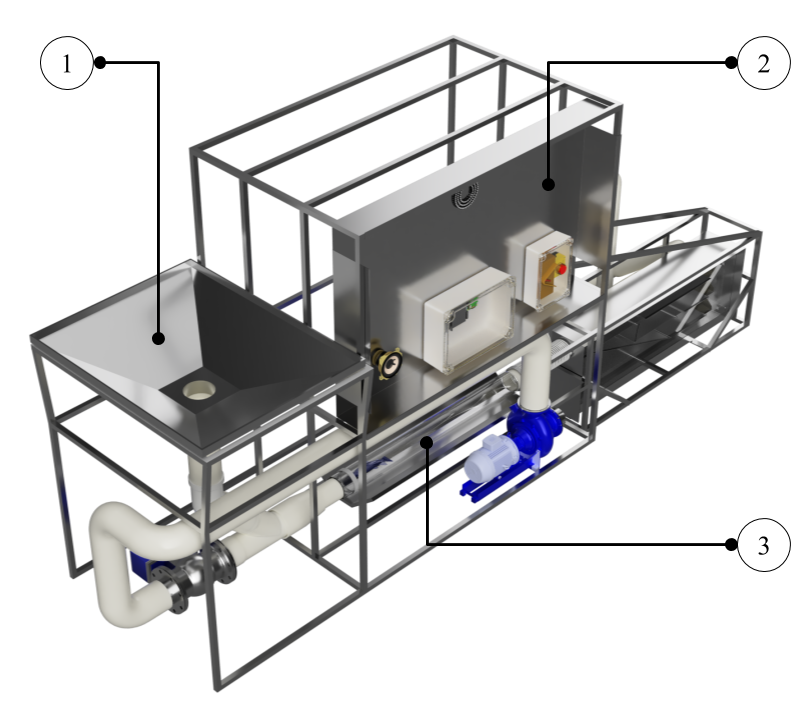
\includegraphics[width=0.75\textwidth]{chapter5/subensambles/diseno integral final.png}
	\caption{Diseño integral de la máquina de clasificación y conteo de truchas.}
	\begin{myflushcenter}
		Fuente: Elaboración propia
	\end{myflushcenter}
	\label{fig:diseno integral}
\end{myfigure}

%% NUEVA SECCIÓN X.X.X
\subsection{Descripción del sistema integral}
\label{ssec:descripcion del sistema integral}

En la Figura \ref{fig:diseno integral} se muestra el diseño mecatrónico integral final donde se enumeran subsecciones: 1. subsistema de recepción, distribución y traslado de truchas; 2. subsistema de control e interacción con el usuario y 3. subsistema de procesamiento de imágenes.

Respecto al diseño conceptual, existen algunas modificaciones en los tipos de dispositivos por características técnicas detectadas en el desarrollo de ingeniería del sistema: el cambio del servomotor por un mecanismo de motor a pasos con leva-seguidor que disminuye el desgaste por el sentido de giro; la batería ya no es parte del sistema, el operario debe suministrar la energía necesaria; el adicional de una cámara para el seguimiento de la trayectoria de truchas en el mecanismo de distribución; la variación de el uso de un microcontrolador a microprocesador debido a la potencia computacional requerida; el cambio de bombas sumergibles a bombas de agua por la eficiencia y potencia necesaria en el proyecto\footnote{El precio de las bombas sumergibles sube considerablemente correspondiente a la potencia requerida.}; remoción de la reja al inicio accionada por un motor debido al coste de implementación y reemplazo con un tapón de plástico; cambio de nombre del interruptor de tipo hongo a interruptor de suministro de energía; aumento del máximo peso admisible según requisito a 400 kg. debido al empleo de plataformas flotantes de alta capacidad de flotación en lugar de su uso en botes de 3 metros de largo.


%\textcolor{blue}{[BORRADOR] INGRESAR AQUÍ CAMBIOS REALIZADOS [/BORRADOR]}\\

La máquina clasificadora y contadora de truchas (CCT), y su sistema respectivo tienen como función principal recepcionar truchas mediante una tolva, procesar la clasificación, conteo y distribución hacia tres jaulas flotantes en medio de la Laguna de Paucarcocha.\footnote{\cite{DiazVergara2020}} La máquina se sitúa sobre el agua y es empleada por un operario, que se encarga de extraer truchas con una sacadera telescópica\footnote{También llamada cal-cal.}. En las siguientes páginas se analizan dos puntos generales concernientes al sistema: arquitectura de hardware y la selección de materiales de fabricación por subsistema.

%% NUEVO SUBSECCION X.X.X.X
\subsubsection{Arquitectura de hardware}

En la Figura \ref{fig:arquitectura de hardware del sistema} se muestra la propuesta de arquitectura de hardware. Esta arquitectura muestra las entradas de energía del sistema, su redistribución a cada componente, el control asociado a cada pieza mediante el subsistema de control y los protocolos o energía asociado a cada par de bloques. Además, el tipo de conexión se detalla en la leyenda. 

\begin{myfigure}[H]
	\footnotesize\centering
	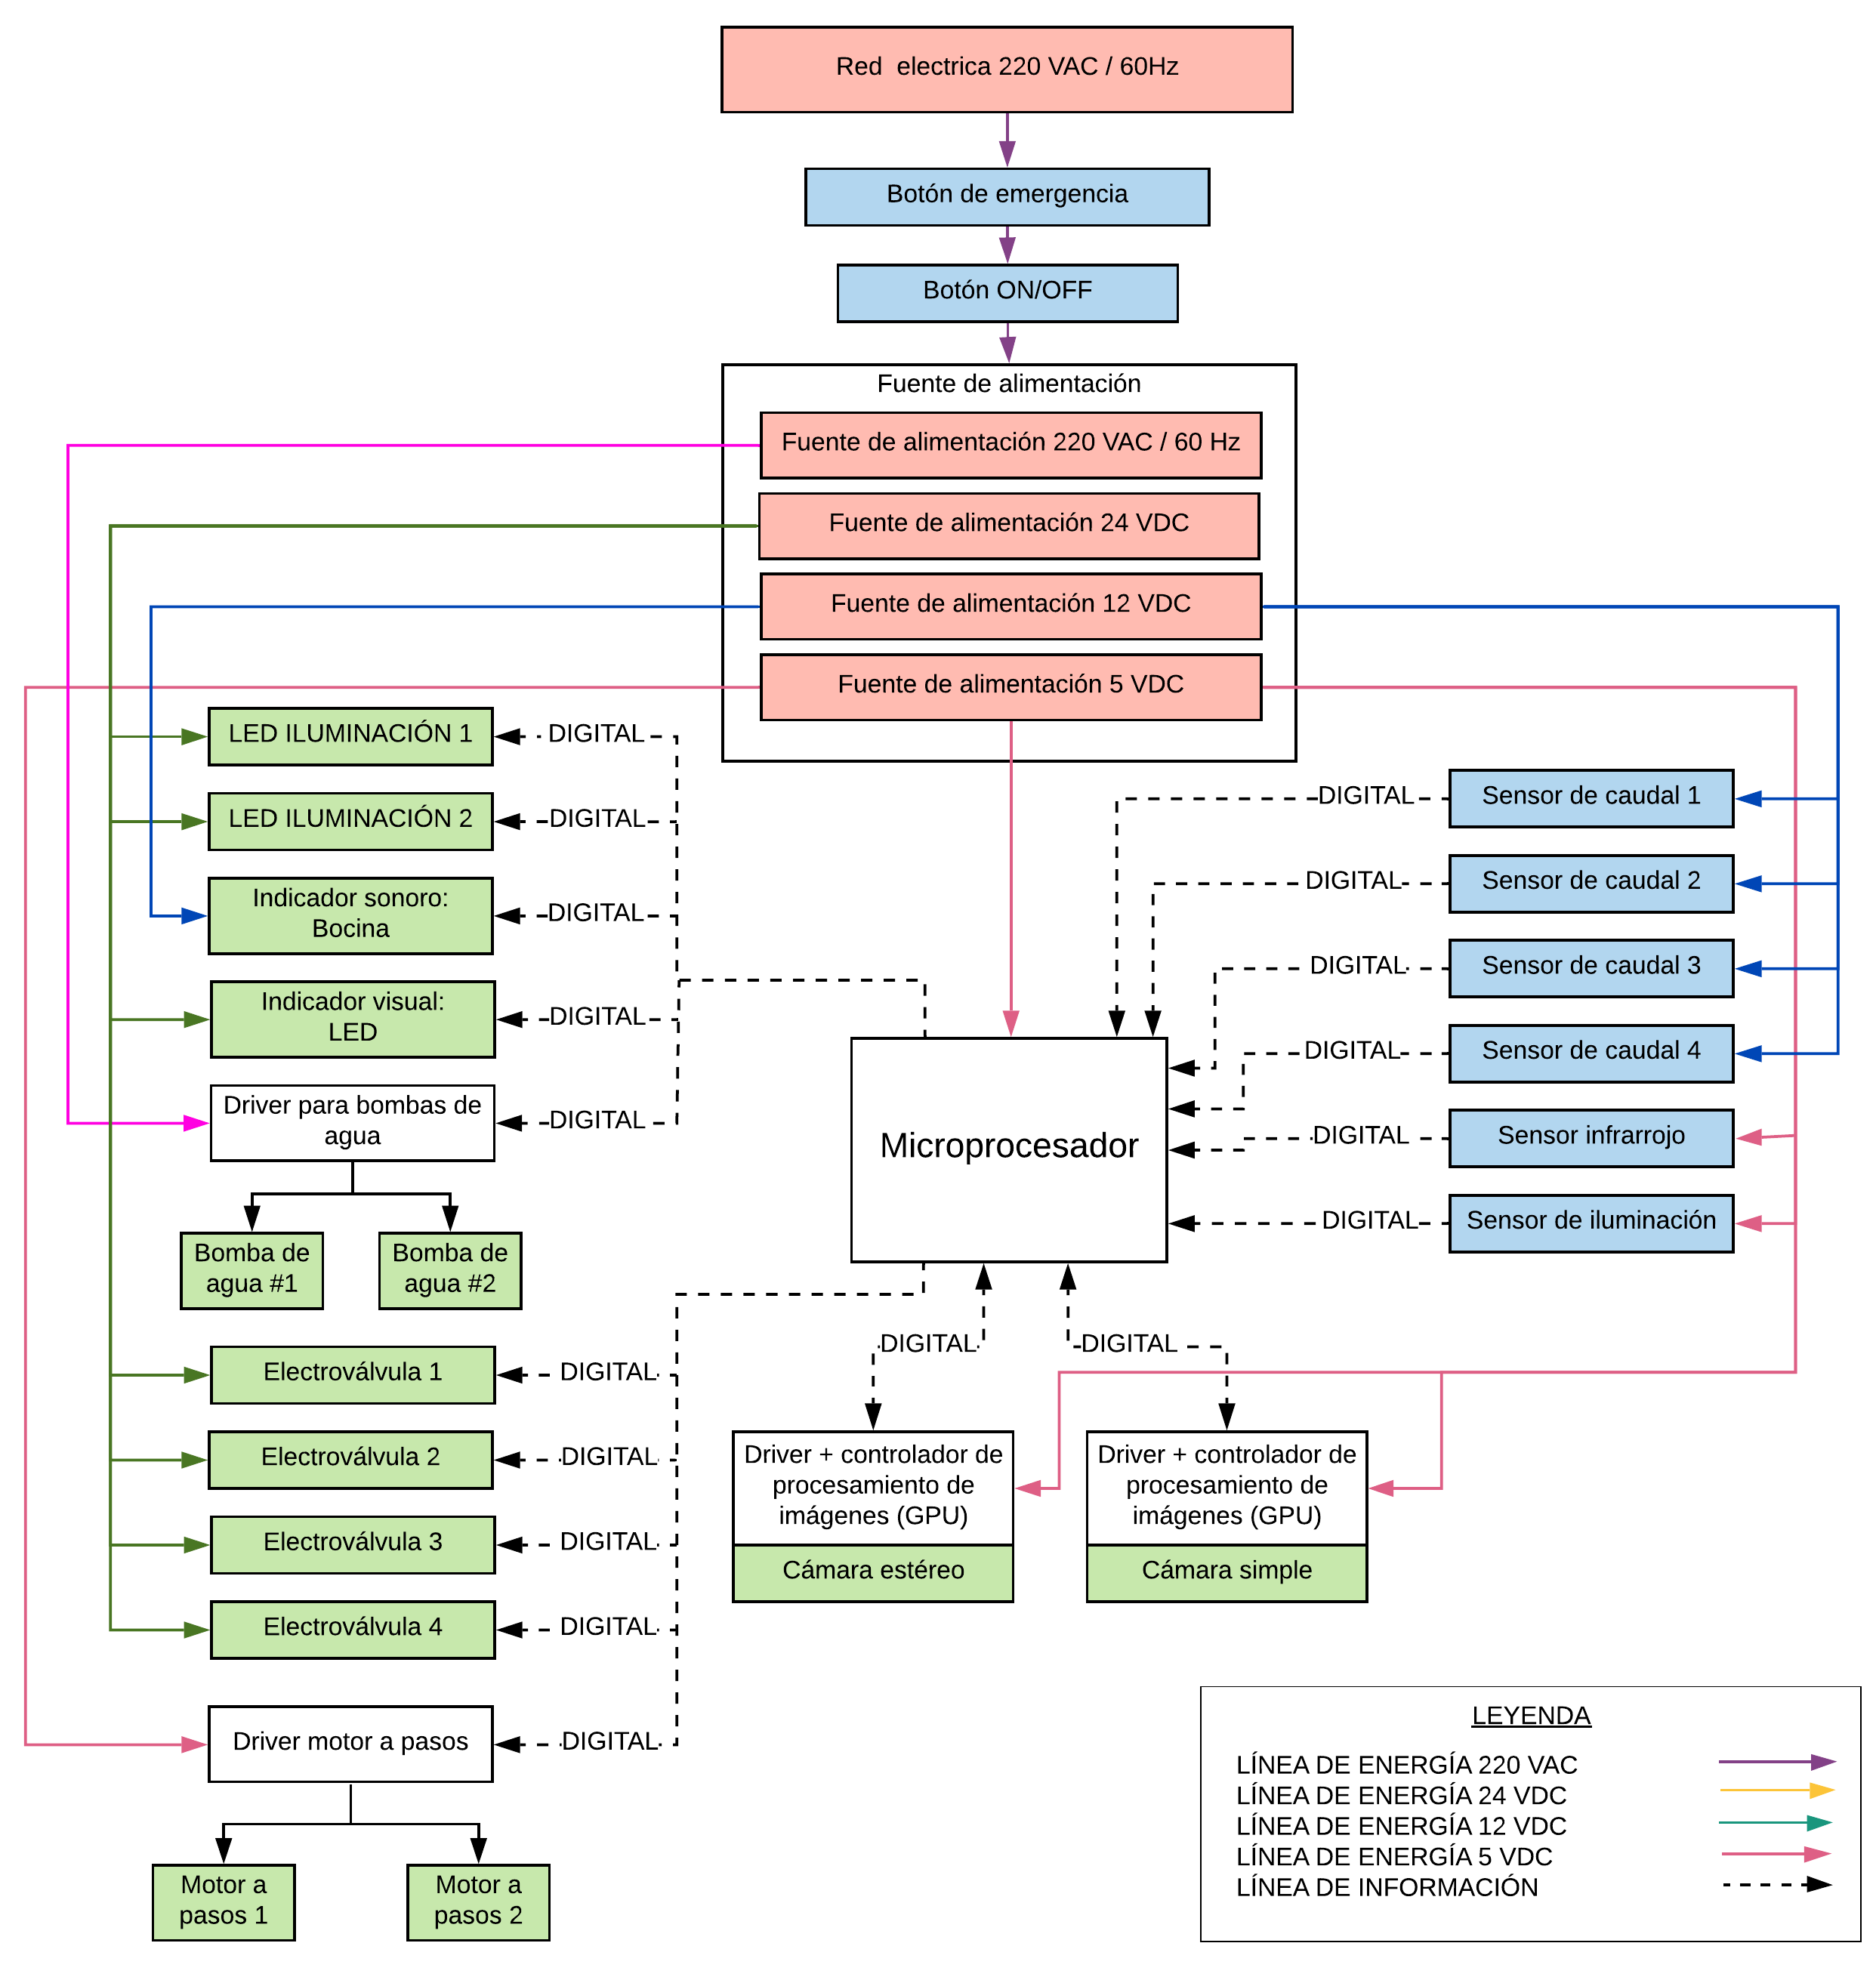
\includegraphics[width=0.90\textwidth]{chapter5/arquitectura de hardware del sistema.png}
	\caption{Arquitectura de hardware del sistema}
	\begin{myflushcenter}
		Fuente: Elaboración propia.
	\end{myflushcenter}
	\label{fig:arquitectura de hardware del sistema}
\end{myfigure}

%% NUEVO SUBSECCION X.X.X.X
\subsubsection{Selección de materiales de fabricación}
\label{sssec:seleccion de materiales de fabricacion}

Cada subsistema posee mecanismos que se rigen por un material en general, esto incluye a las partes principales del subsistema. Sin embargo, no considera el material de tornillos, ajustes o dispositivos similares. Existen así mismos requisitos que se pueden generalizar para todos los subsistemas por el entorno de trabajo a la que estará sometida la máquina detallados en la \textit{"Lista de requerimientos"} \footnote{\cite{DiazVergara2020}.}. Basado en dichas demandas, cada subsistema es analizado y presentado con dos alternativas posibles de materiales. Consecuentemente, se elige un material decisivo para ser empleado bajo el sustento técnico que se explicará en los siguientes párrafos.

\begin{itemize}
	\item \textbf{Subsistema de recepción y traslado de truchas:} Cuenta con dos mecanismos; recepción de truchas y tuberías de traslado. El primero debe recepcionar a las truchas y dirigirlas al mecanismo de tuberías. El segundo debe trasladar a las truchas de un punto a otro de la máquina mediante las tuberías. En la Tabla \ref{tab:tabla comparativa de propiedades entre aluminio vs acero inoxidable} se comparan técnicamente las propiedades mecánicas, térmicas y ópticas de dos materiales.
	
	\begin{mytable}[H]
		\footnotesize\centering
		\caption{Tabla comparativa de propiedades entre $Aluminio$ vs $Acero \quad Inoxidable$}
		\label{tab:tabla comparativa de propiedades entre aluminio vs acero inoxidable}
		\begin{tabular}{|l|c|c|}
			\hline
			\multicolumn{1}{|c|}{\textbf{Propiedad}} & \textbf{Aluminio} & \textbf{Acero Inoxidable} \\ \hline
			Módulo de Young ($GPa$) & 69 & 200 \\ \hline
			Esfuerzo de fatiga $Y$ ($MPa$) & 58-110 & 210-430 \\ \hline
			Resistencia a la tracción ($MPa$) & 130-410 & 520-1180 \\ \hline
			Temperatura máxima mecánica (°$C$) & 650 & 590 \\ \hline
			Conductividad térmica ($W/m-K$) & 170 & 15 \\ \hline
			Expansión térmica (${\mu}m/m-K$) & 24 & 16 \\ \hline
			Conductividad eléctrica ($\%$) & 43 & 2.3 \\ \hline
			Densidad ($g/cm^3$) & 2.7 & 7.9 \\ \hline
		\end{tabular}
		\begin{myflushcenteraftertable}
			*Terminología técnica de los materiales: Aluminio 6061, Acero Inoxidable AISI 306 .\\		
			Fuente: \cite{MakeItFrom2020}.
		\end{myflushcenteraftertable}
	\end{mytable}

	El material escogido es Aluminio 6061 por tener una densidad menor, facilidad de realizar juntas de soldadura, y aunque tenga menor resistencia mecánica cumple con los requerimientos mínimos asociados al subsistema mencionado.
	
	\item \textbf{Subsistema de procesamiento de imágenes:} Cuenta con los mecanismos de tuberías y juego de espejos. El primero debe brindar a la cámara suficiente transparencia para obtener una fotografía adecuada. El segundo debe brindar a la cámara más perfiles del cuerpo que es trasladado por la tubería. En la Tabla \ref{tab:tabla comparativa de propiedades entre pmma vs pvdf vs petg} se compara técnicamente las propiedades mecánicas, térmicas y ópticas de tres materiales.
	
	\begin{mytable}[H]
		\footnotesize\centering
		\caption{Tabla comparativa de propiedades entre $PMMA$, $PVDF$ y $PETG$}
		\label{tab:tabla comparativa de propiedades entre pmma vs pvdf vs petg}
		\begin{tabular}{|l|c|c|c|}
			\hline
			\multicolumn{1}{|c|}{\textbf{Propiedad}} & \multicolumn{1}{c|}{\textbf{PMMA}} & \textbf{PVDF}& \textbf{PETG} \\ \hline
			Resistencia al impacto: con muescas ($J/m$) & 74 & 180 & 77  \\ \hline
			Expansión térmica (${\mu}m/m-K$)  & 76 & 120 & 68 \\ \hline
			Densidad ($g/cm^3$) & 1.2 & 1.8  & 1.3 \\ \hline
			Resistencia al peso  & 32 & 20 & 25 \\ \hline
			Alargamiento a la rotura ($ \% $) & 4 & 49 & 53 \\ \hline
			Incidencia de luz trasmitida ($ \% $) & 92 & - & - \\ \hline
			Índice de refracción & 1.5 & 1.4 & 1.6\\ \hline			
		\end{tabular}
		\begin{myflushcenteraftertable}
			*Terminología técnica de los materiales: Polimetilmetacrilato (Acrílico)(PMMA), Fluoruro de polivinilideno (PVDF), Tereftalato de polietileno modificado con glicol (PETG).\\		
			Fuente: \cite{Brydson1999,Berins1991,Harper2000,MakeItFrom2020}.
		\end{myflushcenteraftertable}
	\end{mytable}

	Tanto el PMMA como el PETG tienen menores propiedades mecánicas que PVDF, pero en cuanto a densidad los materiales mencionados son más livianos comparados con el PVDF. En cuanto a las propiedades ópticas, el PMMA tiene un índice de refracción mayor que el PVDF pero menor que el PETG. Sin embargo, la el PMMA es el material más usado en propósitos ópticos comparado con los otros materiales mencionados. El PMMA transparente se puede encontrar en el mercado nacional e internacional por lo que se opta por este material para el subsistema mencionado. En el caso del juego de espejos, las propiedades ópticas son primordiales, por lo que se escoge PMMA.
	
	\item \textbf{Subsistema de procesamiento de suministro de energía y subsistema de control e interacción con el usuario:} Los materiales son propios de los dispositivos electrónicos comerciales dependientes de la tecnología que se selecciona, por lo que se omite una clasificación de materiales en estos subsistemas.
	
	%\item \textbf{:} Los materiales son propios de los dispositivos que serán adquiridos.
	
	\item \textbf{Subsistema de flotación:} Cuenta con dos mecanismos; armadura y flotadores. El primero debe funcionar como esqueleto para los otros subsistemas y del mismo. El segundo debe mantener el sistema a flote. En la Tabla \ref{tab:tabla comparativa de propiedades entre hdpe vs pvcu} se compara técnicamente las propiedades mecánicas, térmicas y ópticas de dos materiales.
	
	\begin{mytable}[H]
		\footnotesize\centering
		\caption{Tabla comparativa de propiedades entre $HDPE$ vs $PVC-U$}
		\label{tab:tabla comparativa de propiedades entre hdpe vs pvcu}
		\begin{tabular}{|l|c|c|}
			\hline
			\multicolumn{1}{|c|}{\textbf{Propiedad}} & \textbf{HDPE} & \textbf{PVC-U} \\ \hline
			Densidad ($g/cm^3$) & 1.0-1.3 & 1.4 \\ \hline
			Elongación a rotura ($\%$) & 2.5-100 & 58 \\ \hline
			Resistencia al impacto ($J/m$) & 50-260 & 360 \\ \hline
			Resistencia al peso: Flexión & 19-32 & 20 \\ \hline
			Resistencia a la tracción ($MPa$) & 24-80 & 47 \\ \hline
		\end{tabular}
		\begin{myflushcenteraftertable}
			*Terminología técnica de los materiales: Polietileno de alta densidad (HDPE), Cloruro de polivinilo no plastificado (Rígido) (uPVC, PVC-U)\\		
			Fuente: \cite{Brydson1999,Berins1991,Harper2000,MakeItFrom2020}.
		\end{myflushcenteraftertable}
	\end{mytable}
	
	En los flotadores es crucial las propiedades mecánicas, ya que en caso de falla puede hundir todo el sistema. La búsqueda de un material con baja densidad, alta resistencia a la tracción, impacto y al peso determinan el material escogido como HDPE. Además dicho material es comercializado nacionalmente e internacionalmente. De forma similar, la armadura debe poseer buenas propiedades mecánicas y por eso se selecciona Acero Inoxidable.
	
\end{itemize}

Finalmente, en las Tablas \ref{tab:tabla comparativa de propiedades entre aluminio vs acero inoxidable}, \ref{tab:tabla comparativa de propiedades entre pmma vs pvdf vs petg} y \ref{tab:tabla comparativa de propiedades entre hdpe vs pvcu} se comparan diversos materiales para el correspondiente subsistema. Los materiales de fabricación finales para cada subsistema se muestran en la Tabla \ref{tab:materiales de fabricacion por subsistema}, fueron seleccionados por su superioridad en las propiedades técnicas que son valoradas en este proyecto. 

\begin{savenotes}
	\begin{mytable}[H]
		\footnotesize\centering
		\caption{Materiales de fabricación por subsistema}
		\label{tab:materiales de fabricacion por subsistema}
		\begin{tabular}{|l|c|c|}
			\hline
			\multicolumn{1}{|c|}{\textbf{Subsistema}} & \multicolumn{1}{c|}{\textbf{Mecanismo}} & \textbf{Material} \\ \hline
			Recepción y traslado de truchas      & Recepción de truchas   & Aluminio  \\ \hline
			Recepción y traslado de truchas      & Tuberías de traslado   & PVC-U    \\ \hline
			Procesamiento de imágenes            & Tubería                & PMMA  \\ \hline
			Procesamiento de imágenes            & Juego de espejos       & PMMA  \\ \hline
			Suministro de energía                & \multicolumn{1}{c|}{-} & -    \\ \hline
			Control e interacción con el usuario & \multicolumn{1}{c|}{-} & -  \\ \hline
			Flotación                            & Armadura               & Acero Inoxidable \\ \hline
			Flotación                            & Flotadores             & HDPE  \\ \hline
		\end{tabular}
		\begin{myflushcenteraftertable}
		*Terminología técnica de los materiales: Cloruro de polivinilo no plastificado (Rígido) (uPVC, PVC-U), Polimetilmetacrilato ISO 24026-1:2020\footnote{\href{https://www.iso.org/standard/77547.html}{Estándar ISO detallado}. Antecesor: 8257-1:1998. Estándar ASTM: D788-96} (Acrílico) (PMMA), Polietileno de alta densidad (HDPE), Acero Inoxidable AISI 306 , Aluminio 6061 (AL), Fluoruro de polivinilideno (PVDF).\\	
		Fuente: Elaboración propia.
		\end{myflushcenteraftertable}
	\end{mytable}
\end{savenotes}

%% NUEVA SECCIÓN X.X.X
\subsection{Repositorios de código fuente}

Los códigos de los sistemas, algoritmos y otros se almacenan de forma ordenada en repositorios que permiten el versionado, descentralización y disponibilidad de la información para poder reproducir, editar y mejorar los resultados por otras personas. En la Tabla

\begin{mytable}[H]
	\footnotesize\centering
	\caption{Lista de planos de subensamble.}
	\label{tab:lista de repositorios}
	\begin{tabular}{|l|l|}
		\hline
		\multicolumn{1}{|c|}{\textbf{Descripción}} & \multicolumn{1}{c|}{\textbf{Enlace}} \\ \hline
		\textbf{Plantilla de tesis \LaTeX} & \href{https://github.com/ZurMaD/plantilla_tesis_pucp}{https://github.com/ZurMaD/plantilla\_tesis\_pucp}  \\ \hline
		\textbf{Presente tesis} & \href{https://github.com/ZurMaD/tesis_pregrado_pucp}{https://github.com/ZurMaD/tesis\_pregrado\_pucp}  \\ \hline
		\textbf{Datasets de peces ($\approx10GB$)} & \href{https://github.com/DZPeru/fish-datasets}{https://github.com/DZPeru/fish-datasets}  \\ \hline
		\textbf{Algoritmo de detección y conteo v3} & \href{https://github.com/DZPeru/fishv3}{https://github.com/DZPeru/fishv3}  \\ \hline	
		\textbf{Prototipo de aplicativo móvil} & \href{https://bit.ly/3ko1nG0}{https://bit.ly/3ko1nG0}  \\ \hline				
	\end{tabular}
	\begin{myflushcenteraftertable}	
		Fuente: Elaboración propia.
	\end{myflushcenteraftertable}
\end{mytable}

%% NUEVA SECCIÓN X.X.X
\subsection{Planos del sistema}
\label{ssec:planos del sistema}

Los planos permiten visualizar el sistema de una forma en particular dependiendo del tipo de plano. El código asociado a cada plano indica el tipo de plano, su nivel respecto a la estructura general: ensamble, subensamble o despiece, y el tamaño de página usado para dicho plano. En las Tablas \ref{tab:lista de planos de ensamble y subensamble} y \ref{tab:lista de planos de subensamble} se detalla el código junto con la descripción. Dónde: \textit{E} es Ensamble, \textit{SE} es Subensamble, \textit{D} es despiece, los dígitos seguidos son alfanuméricos que van del 0 a la Z y es su agrupación es similar a la organización en cascada, y finalmente el tamaño de página.\footnote{Por ejemplo: D4587-A3 sería un despiece para el componente que pertenece al subensamble 4000, dentro del dispositivo 0500 y 0080. Además de ser el sétimo componente dentro del dispositivo.}

%% NUEVO SUBSECCION X.X.X.X
\subsubsection{Lista de planos de ensamble}

El plano de ensamble presenta una visión de los diferentes componentes, cómo son las juntas, incluye un listado de componentes y se proporcionan características técnicas como el  tipo de material y cantidad de componentes similares.\footnote{Adaptado de \cite{Goetsch2010}} En la Tabla \ref{tab:lista de planos de ensamble y subensamble} se muestra la lista de planos de ensamble y subensambles. 

\begin{mytable}[H]
	\footnotesize\centering
	\caption{Lista de planos de ensamble y subensamble sistema.}
	\label{tab:lista de planos de ensamble y subensamble}
	\begin{tabular}{|l|l|}
		\hline
		\multicolumn{1}{|c|}{\textbf{Código de Plano}} & \multicolumn{1}{c|}{\textbf{Descripción}} \\ \hline
		\textbf{E1000-A0}         & Ensamble total  \\ \hline
		\textbf{SE1100-A0}        & Subsistema de recepción de truchas  \\ \hline
		\textbf{SE1200-A2}        & Subsistema de distribución de truchas \\ \hline
		\textbf{SE1300-A0}        & Subsistema de traslado de truchas \\ \hline
		\textbf{SE1400-A0}        & Subsistema de procesamiento de imágenes \\ \hline
		\textbf{SE1500-A0}        & Subsistema de control e interacción con el usuario\\ \hline
		\textbf{SE1110-A3}        & Tolva de recepción \\ \hline
		\textbf{SE1210-A3}        & Distribuidora 1:3 \\ \hline
		\textbf{SE1310-A3}        & Tuberías \\ \hline 
		\textbf{SE1510-A3}        & Panel de control \\ \hline
	\end{tabular}
	\begin{myflushcenteraftertable}	
		Fuente: Elaboración propia.
	\end{myflushcenteraftertable}
\end{mytable}

\vspace{-1.0 em}
%% NUEVO SUBSECCION X.X.X.X
\subsubsection{Plano de despiece}

El plano de despiece presenta las características técnicas de cada pieza: muestra dimensiones para poder fabricar la pieza. En el presente trabajo se administran, además, subensambles con la finalidad de brindar mayor detalle a cada componente. En la Tabla \ref{tab:lista de planos de subensamble} se muestra la lista de planos de despiece. 

\begin{mytable}[H]
	\footnotesize\centering
	\caption{Lista de planos de subensamble.}
	\label{tab:lista de planos de subensamble}
	\begin{tabular}{|c|l|}
		\hline
		\multicolumn{1}{|c|}{\textbf{Código de Plano}} & \multicolumn{1}{c|}{\textbf{Descripción}} \\ \hline
		\textbf{D1010-A3}         & Estructura de soporte  \\ \hline
		\textbf{D1120-A1}         & Tolva de recepción - Borde \\ \hline
		\textbf{D1130-A3}         & Tolva de recepción - Base de salida \\ \hline
		\textbf{D1211-A1}         & Distribuidora 1:3 - Pared A \\ \hline
		\textbf{D1212-A1}         & Distribuidora 1:3 - Pared B \\ \hline
		\textbf{D1213-A3}         & Distribuidora 1:3 - Tapa de distribuidora \\ \hline
		\textbf{D1214-A3}         & Distribuidora 1:3 - Leva de distribuidora \\ \hline
		\textbf{D1215-A3}         & Distribuidora 1:3 - Lengüeta de salida de tubería \\ \hline
		\textbf{D1216-A3}         & Distribuidora 1:3 - Lengüeta de soporte de servomotor 1 \\ \hline
		\textbf{D1217-A3}         & Distribuidora 1:3 - Lengüeta de soporte de servomotor 2 \\ \hline 
		\textbf{D1217-A3}         & Distribuidora 1:3 - Compuerta mecánica \\ \hline 
		\textbf{D1311-A3}         & Tuberías - Adaptador de entrada de bomba de agua \\ \hline 
		\textbf{D1312-A3}         & Tuberías - Adaptador de salida de bomba de agua \\ \hline 
		\textbf{D1313-A3}         & Tuberías - Adaptador de electroválvula\\ \hline
		\textbf{D1314-A3}         & Tuberías - Reductor de tubería \\ \hline
		\textbf{D1415-A3}         & Procesamiento de imágenes \\ \hline
		\textbf{D1416-A3}         & Procesamiento de imágenes - Tubería \\ \hline
		\textbf{D1417-A3}         & Procesamiento de imágenes - Soporte de cámara estéreo \\ \hline
		\textbf{D1511-A3}         & Panel de control - Caja de control 1 \\ \hline
		\textbf{D1512-A3}         & Panel de control - Caja de control 2 \\ \hline
		\textbf{D1513-A3}         & Panel de control - Soporte \\ \hline
	\end{tabular}
	\begin{myflushcenteraftertable}	
		Fuente: Elaboración propia.
	\end{myflushcenteraftertable}
\end{mytable}



%----------------------------------------------------------------------------------------
%	Capítulo 5 
%----------------------------------------------------------------------------------------

\pagestyle{myportland}
%\pagenumbering{arabic}
\doublespacing
\chapter[\quad\quad\quad\quad ----- Diseño de subsistema de recepción, distribución y traslado de truchas]{\\ Diseño de subsistema de recepción, distribución y traslado de truchas}
\thispagestyle{myportland}

\label{ssec:diseno de subsistema de recepcion, distribucion y traslado de truchas}

Este subsistema consiste en encapsular los mecanismos físicos que están en el ciclo que sigue una trucha dentro de la máquina: tolva, tuberías, bomba de agua, distribución física por mecanismos, caudales apropiados y el control respectivo. Los puntos mencionados se detallan en las siguientes páginas. En la Figura \ref{fig:subsistema de recepción, distribución y traslado de truchas} se muestran los tres sistemas: 1. recepción, 2. distribución y lo restante 3. distribución.

\begin{myfigure}[H]
	\footnotesize\centering
	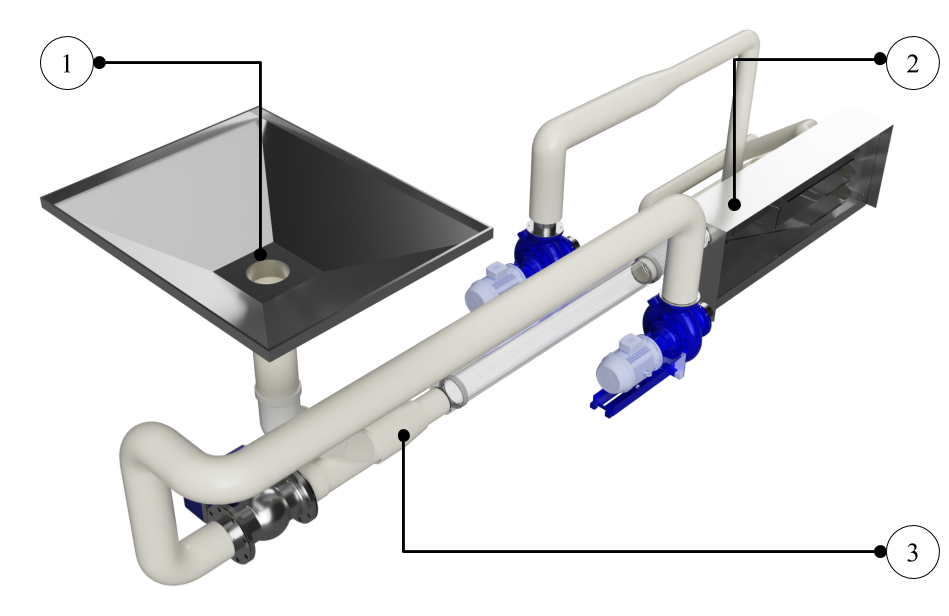
\includegraphics[width=1\textwidth]{chapter5/subensambles/recepcion distribucion y traslado isometrico final.png}
	\caption{Subsistema de recepción, distribución y traslado de truchas}
	\begin{myflushcenter}
		Fuente: Elaboración propia.
	\end{myflushcenter}
	\label{fig:subsistema de recepción, distribución y traslado de truchas}
\end{myfigure}

%% NUEVO SECCION X.X.X.X
\section{Diseño del subsistema de recepción de truchas}

El diseño implica un análisis sobre las situaciones que suceden cuando se realiza el proceso de depositar las truchas. En la Figura \ref{fig:calculo de dimensiones y angulo de la tolva} se analiza dicha situación con la finalidad de escoger un ángulo de elevación de la tolva ($\beta$) adecuado. Respecto a la tolva, se designan los siguientes valores iniciales: $A_{min},B_{min}=200 mm.$; $\beta \in [0;45] ^\circ$; ${tolva}=150 mm.$. Además, debe cumplirse que $A_{max}>B_{max}$ orientado hacia el operario que depositará la trucha.

\begin{myfigure}[H]
	\footnotesize\centering
	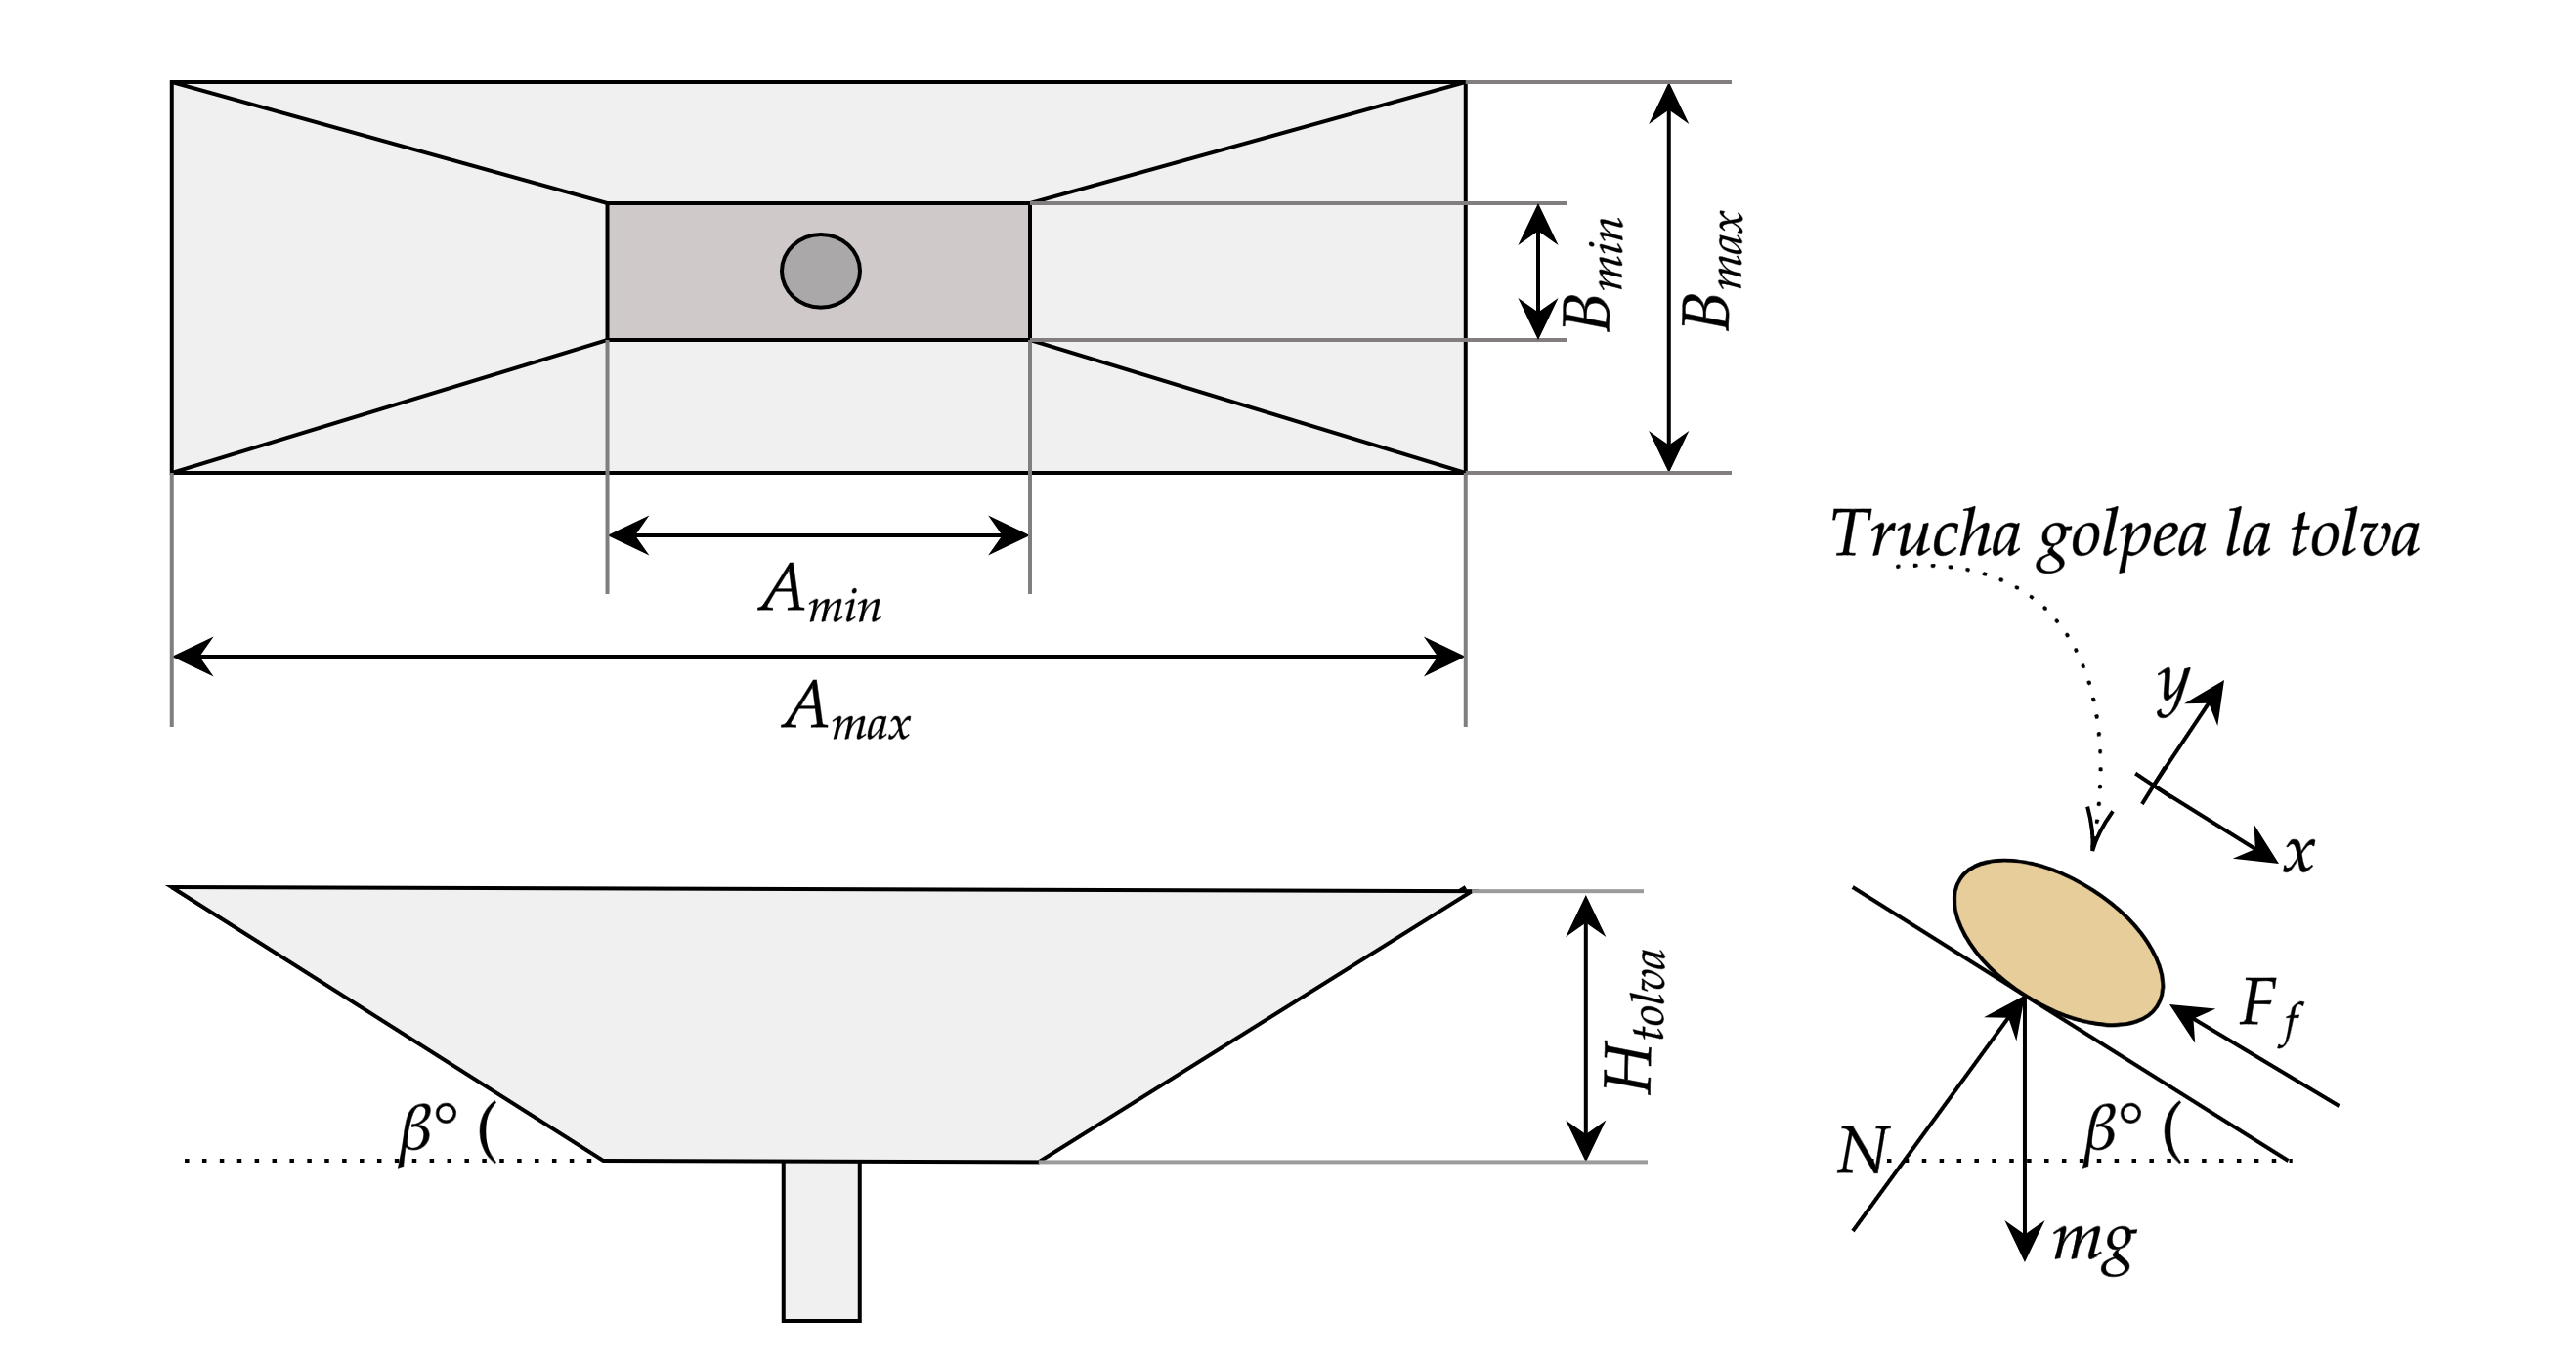
\includegraphics[width=1\textwidth]{chapter5/calculo de dimensiones y angulo de la tolva.png}
	\caption{Cálculo de dimensiones y ángulo de la tolva}
	\begin{myflushcenter}
		Fuente: Elaboración propia.
	\end{myflushcenter}
	\label{fig:calculo de dimensiones y angulo de la tolva}
\end{myfigure}

Parte de la Figura \ref{fig:calculo de dimensiones y angulo de la tolva} muestra el diagrama de cuerpo libre del cual se extrae la fuerza de fricción ($F_{f}$) y la fuerza normal ($N$) que se muestran en la Ecuación \ref{eq:calculo de angulo de la tolva}. Las leyes de Newton se muestran en la Ecuación \ref{eq:leyes de newton}. 

\begin{myequation}\label{eq:leyes de newton}
	\begin{split}
		F_{R}=m*a \\
		\sum_{0}^{n}F_{x,y,z}=0
	\end{split}
\end{myequation}

\begin{myequation}\label{eq:calculo de angulo de la tolva}
	\begin{split}
		F_{f}=\mu*N  \\
		\sum_{}^{}F_{y}=N-mg*cos(\beta)=0
	\end{split}
\end{myequation}

Luego, se reemplazan la Ecuación \ref{eq:calculo de angulo de la tolva} en la Ecuación \ref{eq:leyes de newton} y se obtiene la Ecuación \ref{eq:calculo de angulo de la tolva2}. La variable a despejar es la aceleración en el eje x ($\ddot{x}$).

\begin{myequation}\label{eq:calculo de angulo de la tolva2}
	\begin{split}
		mg*sin(\beta)-F_{f}&=m*\ddot{x} \\
		mg*sin(\beta)-\mu_{k}*mg*cos(\beta)&=m*\ddot{x} \\
		g*sin(\beta)-g*\mu_{k}*cos(\beta)&=\ddot{x}
	\end{split}
\end{myequation}

Para disminuir el impacto de la trucha sobre la tolva o sobre las tuberías interiores se debe disminuir la aceleración de la trucha al ser depositada en la tolva. La Figura \ref{fig:grafico angulo de tolva vs aceleracion} muestra la ecuación que relaciona la aceleración con el ángulo de elevación de la pared de la tolva. Consecuentemente, se escoge un ángulo ($\beta=30^\circ$) para tener una aceleración aproximadamente nula ($\ddot{x}\approx0$). Se considera $\mu_{k}=0.57$ para el material escogido en la sección \ref{sssec:seleccion de materiales de fabricacion}. Consecuentemente, se calculan los valores de $A_{max}\approx{900} mm.$ y $B_{max}\approx{700} mm.$, respectivamente.

% Material escogido Acero inoxidable

\begin{myfigure}[H]
	\footnotesize\centering
	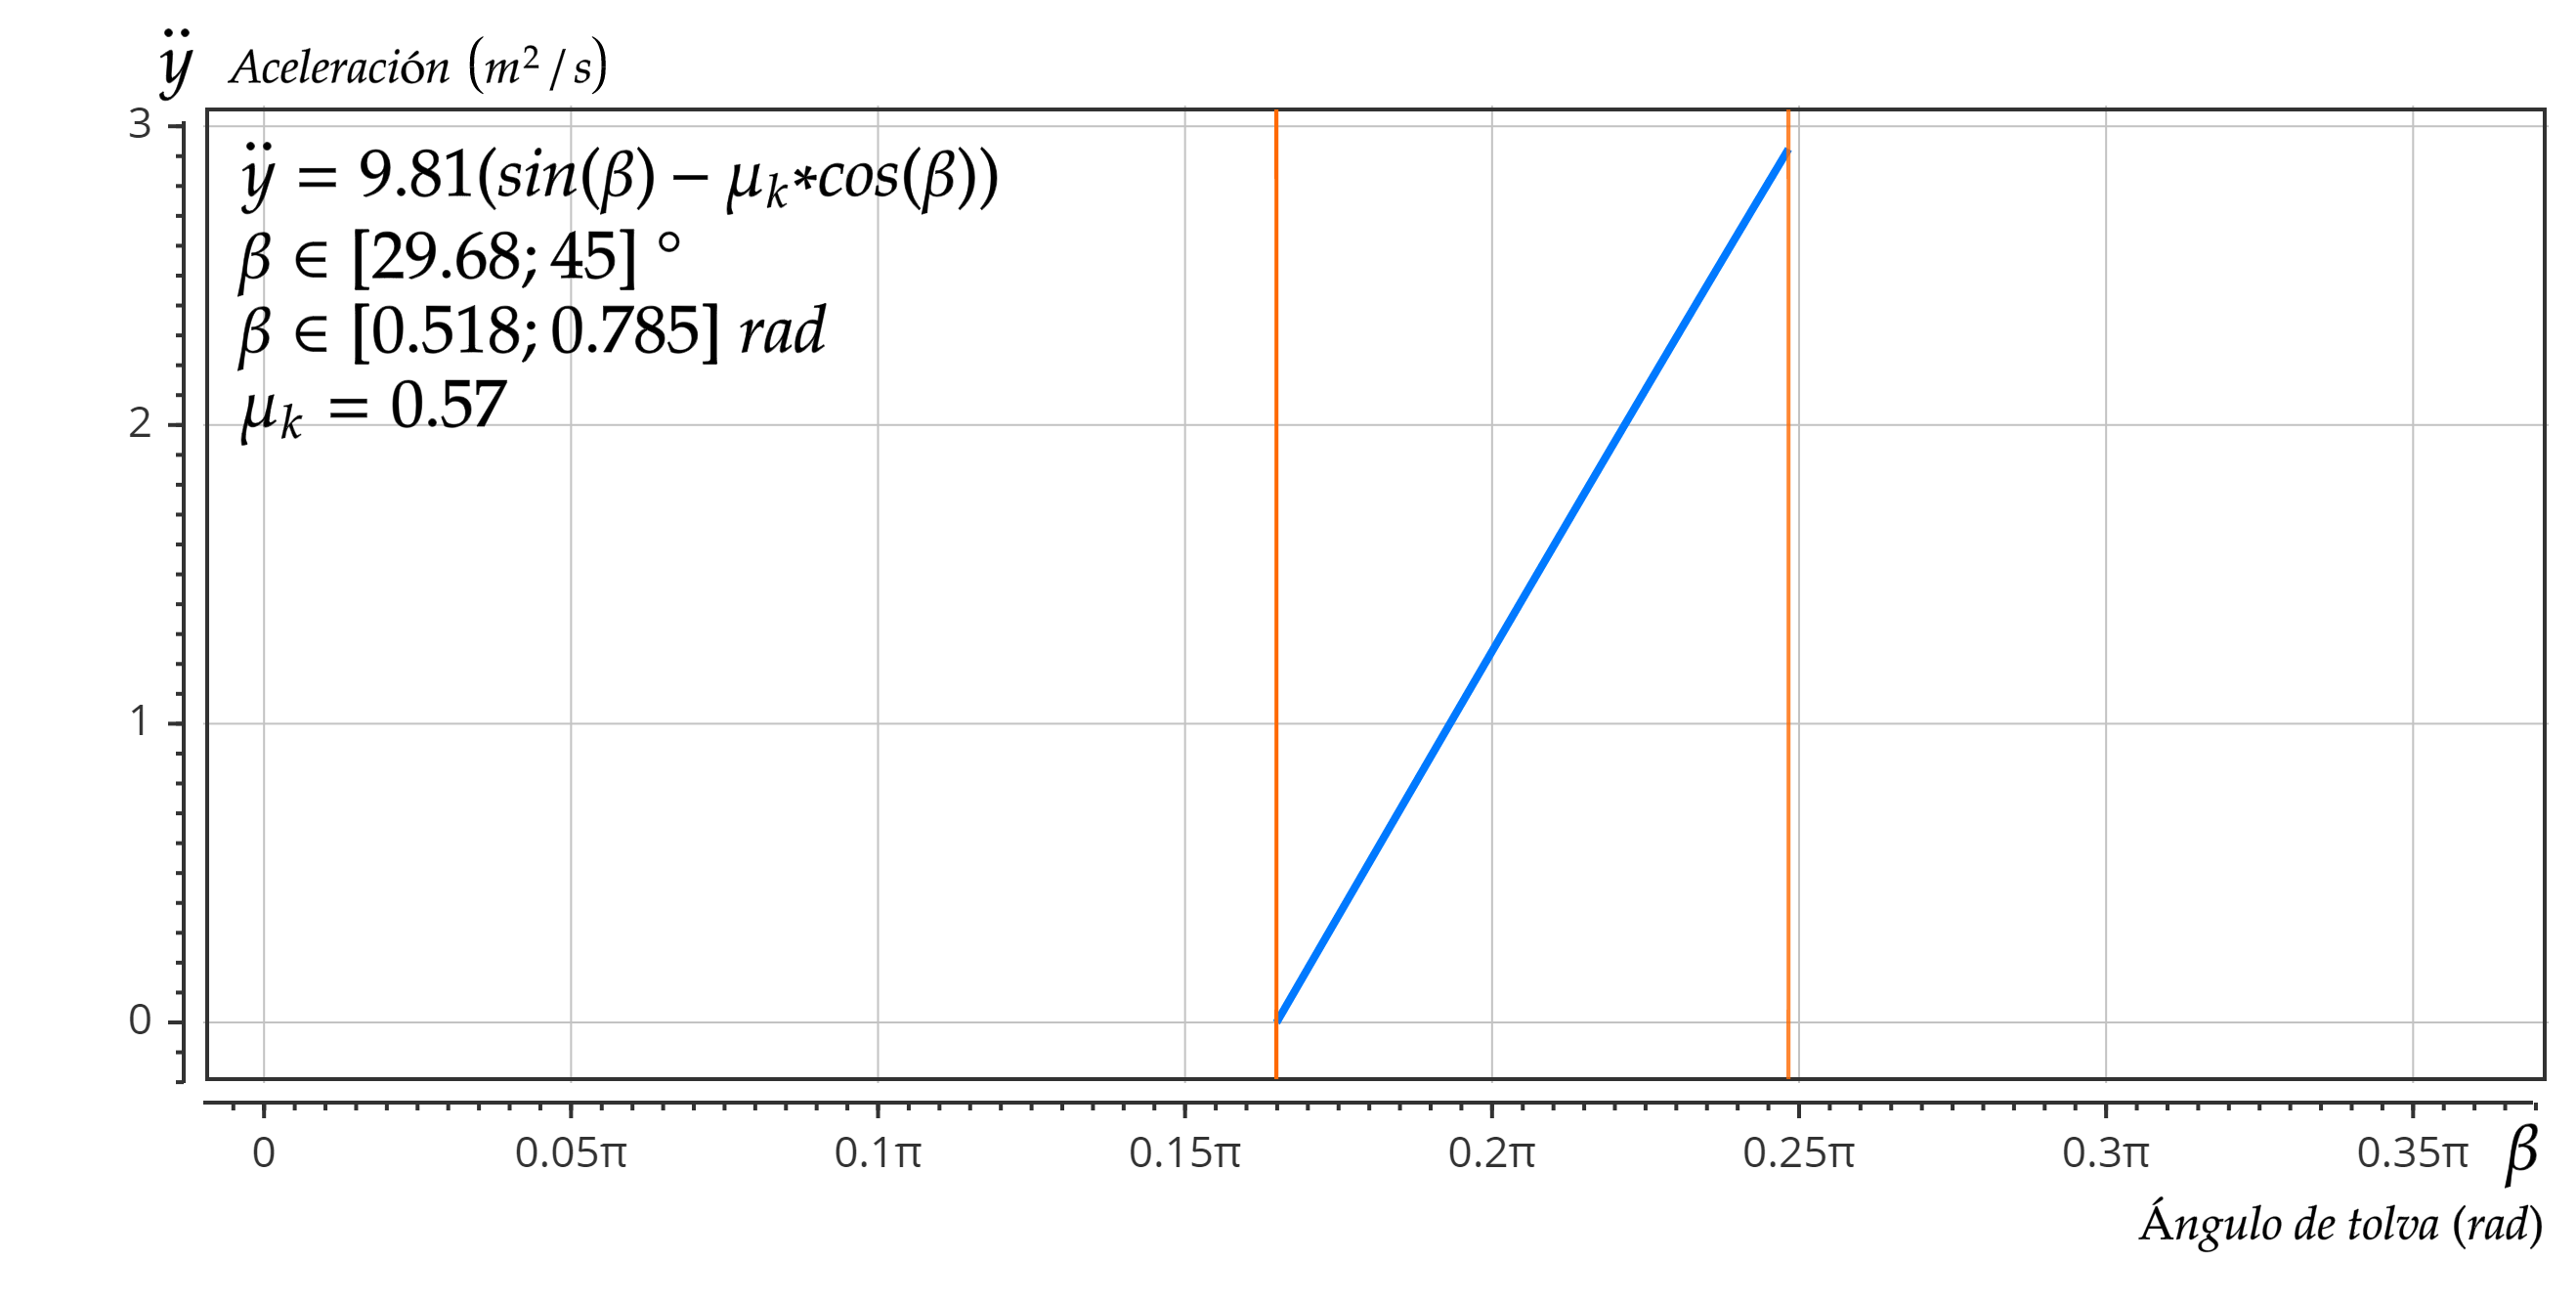
\includegraphics[width=1\textwidth]{chapter5/grafico angulo de tolva vs aceleracion.png}
	\caption{Ángulo de tolva vs aceleración en la trucha}
	\begin{myflushcenter}
		Fuente: Elaboración propia.
	\end{myflushcenter}
	\label{fig:grafico angulo de tolva vs aceleracion}
\end{myfigure}

%% NUEVO SECCION X.X.
\section{Diseño de subsistema de distribución de truchas}

Luego del proceso de procesamiento de imágenes el sistema mediante el algoritmo de clasificación indica al sistema la trayectoria que debe seguir la trucha en tránsito y es accionado por el mecanismo de distribución, mostrado en la Figura \ref{fig:mecanismo de distribucion de truchas}. En la Figura \ref{fig:mecanismo de distribucion de truchas} se enumera sus componentes principales: 1. placa tipo tapa; 2. pared a de la distribuidora; 3. pared b de la distribuidora; 4. placa intermedia; 5. mecanismo de compuerta\footnote{La leva no se muestra adecuadamente en esta vista.}. Dicho mecanismo recibe a la trucha por una única entrada y redirige mediante un juego de compuertas a tres salidas. Finalmente, las truchas son impulsadas al ingresar a tuberías con caudal de agua constante que las transporta hasta las jaulas flotantes correspondientes.

\begin{myfigure}[H]
	\footnotesize\centering
	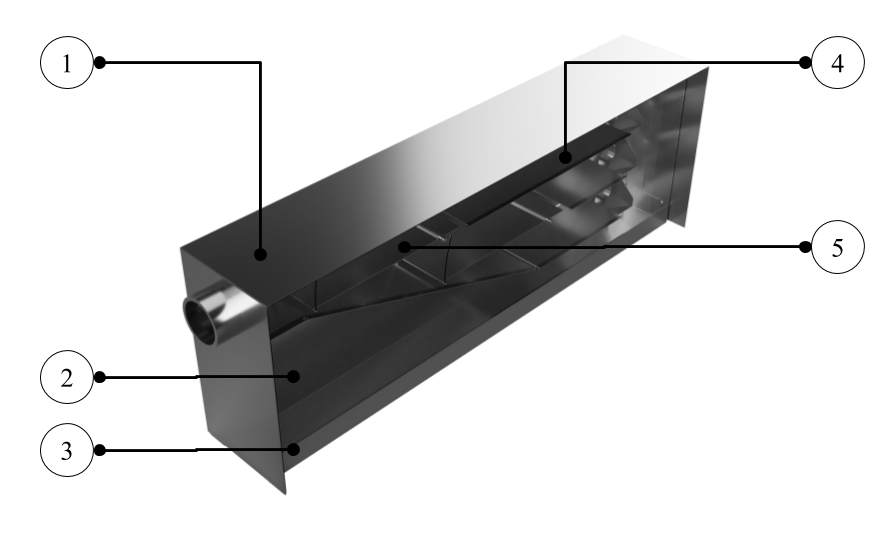
\includegraphics[width=1\textwidth]{chapter5/mecanismo de distribucion de truchas final.png}
	\caption{Mecanismo de distribución de truchas}
	\begin{myflushcenter}
		Fuente: Elaboración propia.
	\end{myflushcenter}
	\label{fig:mecanismo de distribucion de truchas}
\end{myfigure}

%% NUEVO SECCION X.X.X.
\subsection{Selección de mecanismo que acciona la compuerta}
	
La selección del mecanismo que activa la compuerta tiene requisitos técnicos que son muy importantes, de no funcionar puede parar completamente el proceso general, por lo que se realiza una comparación de los posibles mecanismos a utilizar para hacer girar la compuerta de manera cíclica ordenado por el subsistema de control. La comparación conceptual se muestra en la Tabla \ref{tab:tabla comparativa de conceptos de mecanismos para compuerta} y los conceptos de mecanismos analizados se muestran en la Figura \ref{fig:conceptos de mecanismos de distribucion de truchas}.
	
\begin{myfigure}[H]
	\footnotesize\centering
	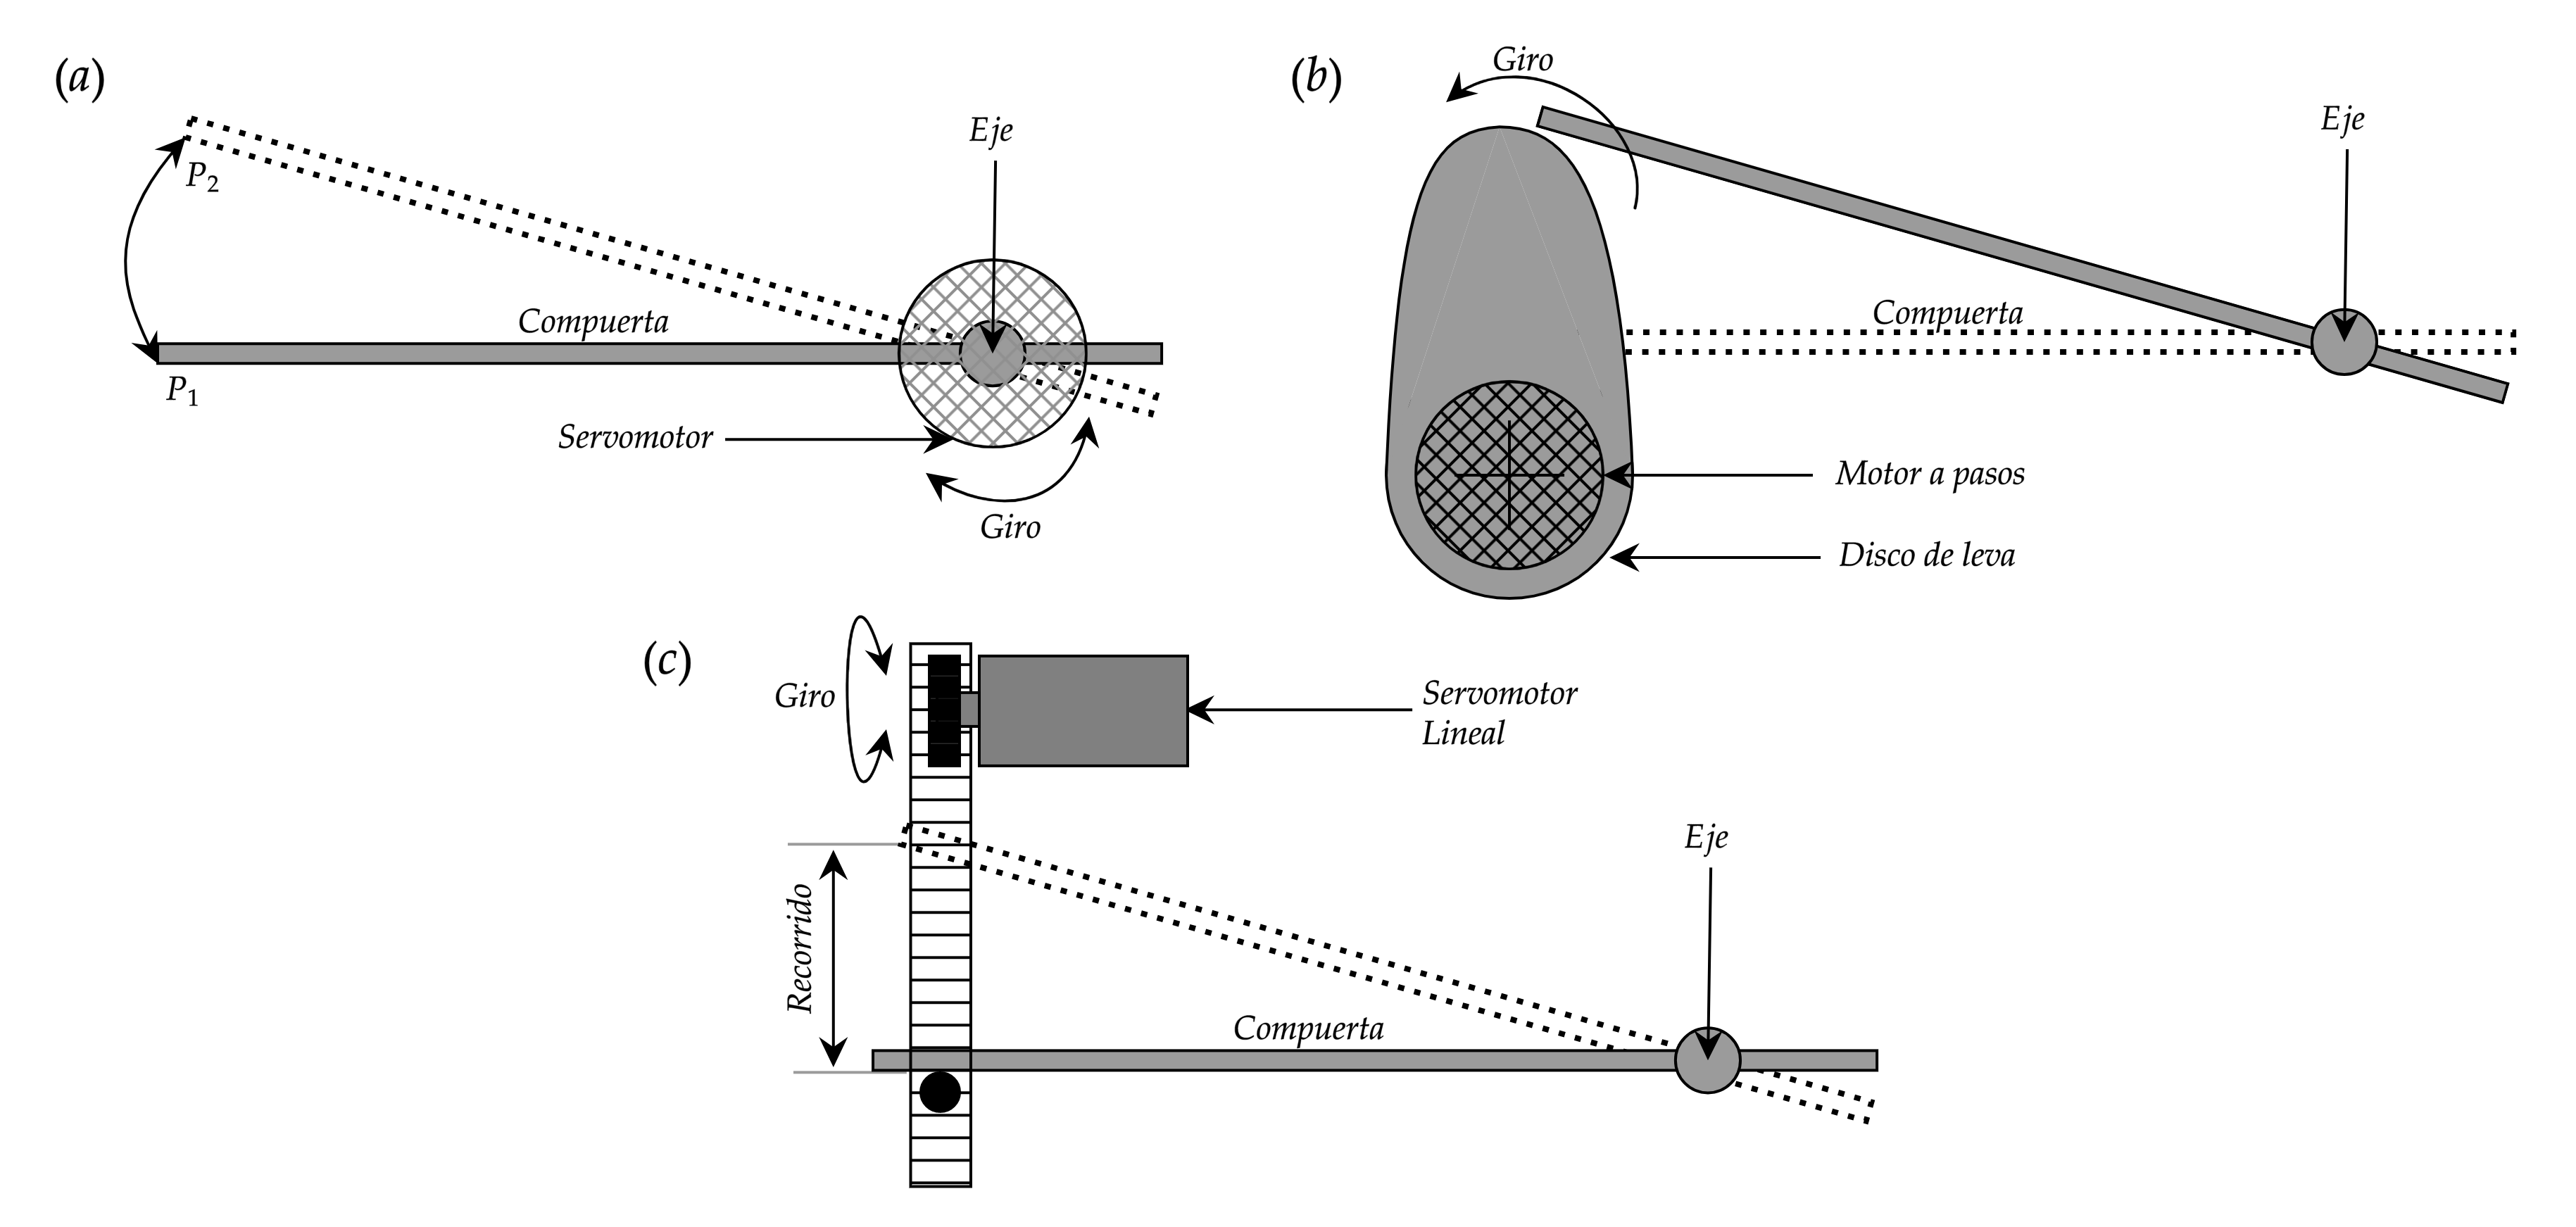
\includegraphics[width=1\textwidth]{chapter5/conceptos de mecanismos de distribucion de truchas.png}
	\caption[Conceptos de mecanismos de distribución de truchas]{(a) Mecanismo de eje servomotor. (b) Mecanismo de tolva y seguidor. (c) Mecanismo de servomotor lineal.}
	\begin{myflushcenter}
		Fuente: Elaboración propia.
	\end{myflushcenter}
	\label{fig:conceptos de mecanismos de distribucion de truchas}
\end{myfigure}
	
El mecanismo inicialmente propuesto (Figura \ref{fig:conceptos de mecanismos de distribucion de truchas}-a) corresponde a un servomotor conectado al eje de la compuerta del sistema de distribución, los apoyos no son representados en las figuras. El sistema, al efectuar cierta cantidad de giros en un periodo largo\footnote{Una jornada diaria de clasificación puede someter al mecanismo a abrir/cerrar la compuerta en $t_{compuerta}\approx1 s.$ durante $t_{jornadaxdia}=6 h.$} presenta un deterioro considerable en el eje del servomotor, por lo que se analiza un mecanismo de leva-seguidor (Figura \ref{fig:conceptos de mecanismos de distribucion de truchas}-b) que traslada el giro fuera del eje, en un solo sentido y se aplica el giro sobre un extremo de la compuerta, el disco de leva está posicionado para brindar un movimiento armónico al extremo de la compuerta. Así también, se considera un mecanismo de servomotor lineal que mediante una traba en la cremallera desplaza la compuerta hasta la posición requerida mediante giros en los dos sentidos.

\begin{savenotes}	
	\begin{mytable}[H]
		\footnotesize\centering
		\caption{Tabla comparativa de conceptos de mecanismos.}
		\label{tab:tabla comparativa de conceptos de mecanismos para compuerta}
		\begin{tabular}{l|c|c|c|c|}
			\cline{2-5}
			\multicolumn{1}{c|}{\textbf{}} & 
			\textbf{\begin{tabular}[c]{@{}c@{}}Requisitos\\ mínimos\end{tabular}} & \begin{minipage}{\mythirdmaxsizeofcontenttable}\begin{myflushcenterinsidetable}
					\textbf{Servomotor de rotación posicional}
			\end{myflushcenterinsidetable}\end{minipage} & 
			\begin{minipage}{\mythirdmaxsizeofcontenttable}\begin{myflushcenterinsidetable}
					\textbf{Leva y seguidor}
			\end{myflushcenterinsidetable}\end{minipage} &
			\begin{minipage}{\mythirdmaxsizeofcontenttable}\begin{myflushcenterinsidetable}
					\textbf{Servomotor lineal}
			\end{myflushcenterinsidetable}\end{minipage} \\ \hline
			%\multicolumn{1}{|l|}{\textbf{Figura}} & - & 
			%Figura \ref{fig:conceptos de mecanismos de distribucion de truchas}-a &
			%Figura \ref{fig:conceptos de mecanismos de distribucion de truchas}-b &
			%Figura \ref{fig:conceptos de mecanismos de distribucion de truchas}-c \\ \hline
			\multicolumn{1}{|l|}{
				\begin{minipage}{\myforthmaxsizeofcontenttable}			
					\textbf{Cantidad de sentidos de giro}
				\end{minipage}
			} & 1 & 2 & 1 & 2 \\ \hline
			\multicolumn{1}{|l|}{
				\begin{minipage}{\myforthmaxsizeofcontenttable}			
					\textbf{Complejidad mecánica\footnote{Basado en cantidad de componentes actuadores.}}
				\end{minipage}
			} & 1 & 1 & 2 & 2 \\ \hline
			\multicolumn{1}{|l|}{
				\begin{minipage}{\myforthmaxsizeofcontenttable}			
					\textbf{Disponibilidad en el mercado\footnote{Basado en el componente más "difícil" de conseguir.Calificación cualitativa: nacional o internacional}}
				\end{minipage}
			} & - & Nacional & Internacional & Nacional \\ \hline
			\multicolumn{1}{|l|}{
				\begin{minipage}{\myforthmaxsizeofcontenttable}			
					\textbf{Torque máximo\footnote{Basado en situación crítica encontrada derivando la ecuación de torque respectivo. Dónde: $d_{eje}$ es la distancia del centro de gravedad de la compuerta al eje, $d_{leva}$ es la distancia del centro del disco de leva hasta la parte más alejada de este y $d_{ser}$ es diámetro del engranaje en el mecanismo piñón-cremallera del servomotor lineal. ($d_{ser}<d_{leva}<d_{eje}$)} ($\overrightarrow{\tau_{max}}$)}	
				\end{minipage}
			} & - & $\approx m*g*d_{eje}$ & $\approx m*g*d_{leva}/2$ & $\approx m*g*d_{ser}/4$ \\ \hline
			%\multicolumn{1}{|l|}{
			%	\begin{minipage}{\myforthmaxsizeofcontenttable}			
			%		\textbf{Desgaste\footnote{Calificación cualitativa: bajo, medio o alto.}}
			%	\end{minipage}
			%} & - & Alto & Bajo & Medio \\ \hline
			\multicolumn{1}{|l|}{
				\begin{minipage}{\myforthmaxsizeofcontenttable}			
					\textbf{Acoplamiento al sistema\footnote{Basado en cantidad de componentes adicionales necesarios para implementar. }}
				\end{minipage}
			} & 1 & 1 & 2 & 3 \\ \hline
			\multicolumn{1}{|l|}{
				\begin{minipage}{\myforthmaxsizeofcontenttable}			
					\textbf{Actuador que genera ruido\footnote{Componente que genera sonido.}}
				\end{minipage}
			} & - & Servomotor rotatorio & Motor a pasos & Servomotor lineal \\ \hline
		\end{tabular}
		\begin{myflushcenteraftertable}	
			Fuente: Elaboración propia.
		\end{myflushcenteraftertable}
	\end{mytable}
\end{savenotes}	

El mecanismo escogido es el leva y seguidor ya que solo es necesario su giro en un sentido, lo cual disminuye el desgaste, se acopla al sistema sin implementar más soportes que los otros mecanismos, no genera ruido y su fabricación, en caso no se encuentre en el mercado peruano, se puede realizar en un taller nacional.  	

%% NUEVO SECCION X.X.X.
\subsection{Diseño de mecanismo que acciona la compuerta}
	
En cuanto al mecanismo determinado, se realiza una análisis simple para determinar la forma que tendrá el disco de leva (\ref{fig:mecanismo compuerta}-b) y con ese fin se realiza un diagrama de cuerpo libre (\ref{fig:mecanismo compuerta}-a) que permite analizar las fuerzas sobre los cuerpos.

\begin{myfigure}[H]
	\footnotesize\centering
	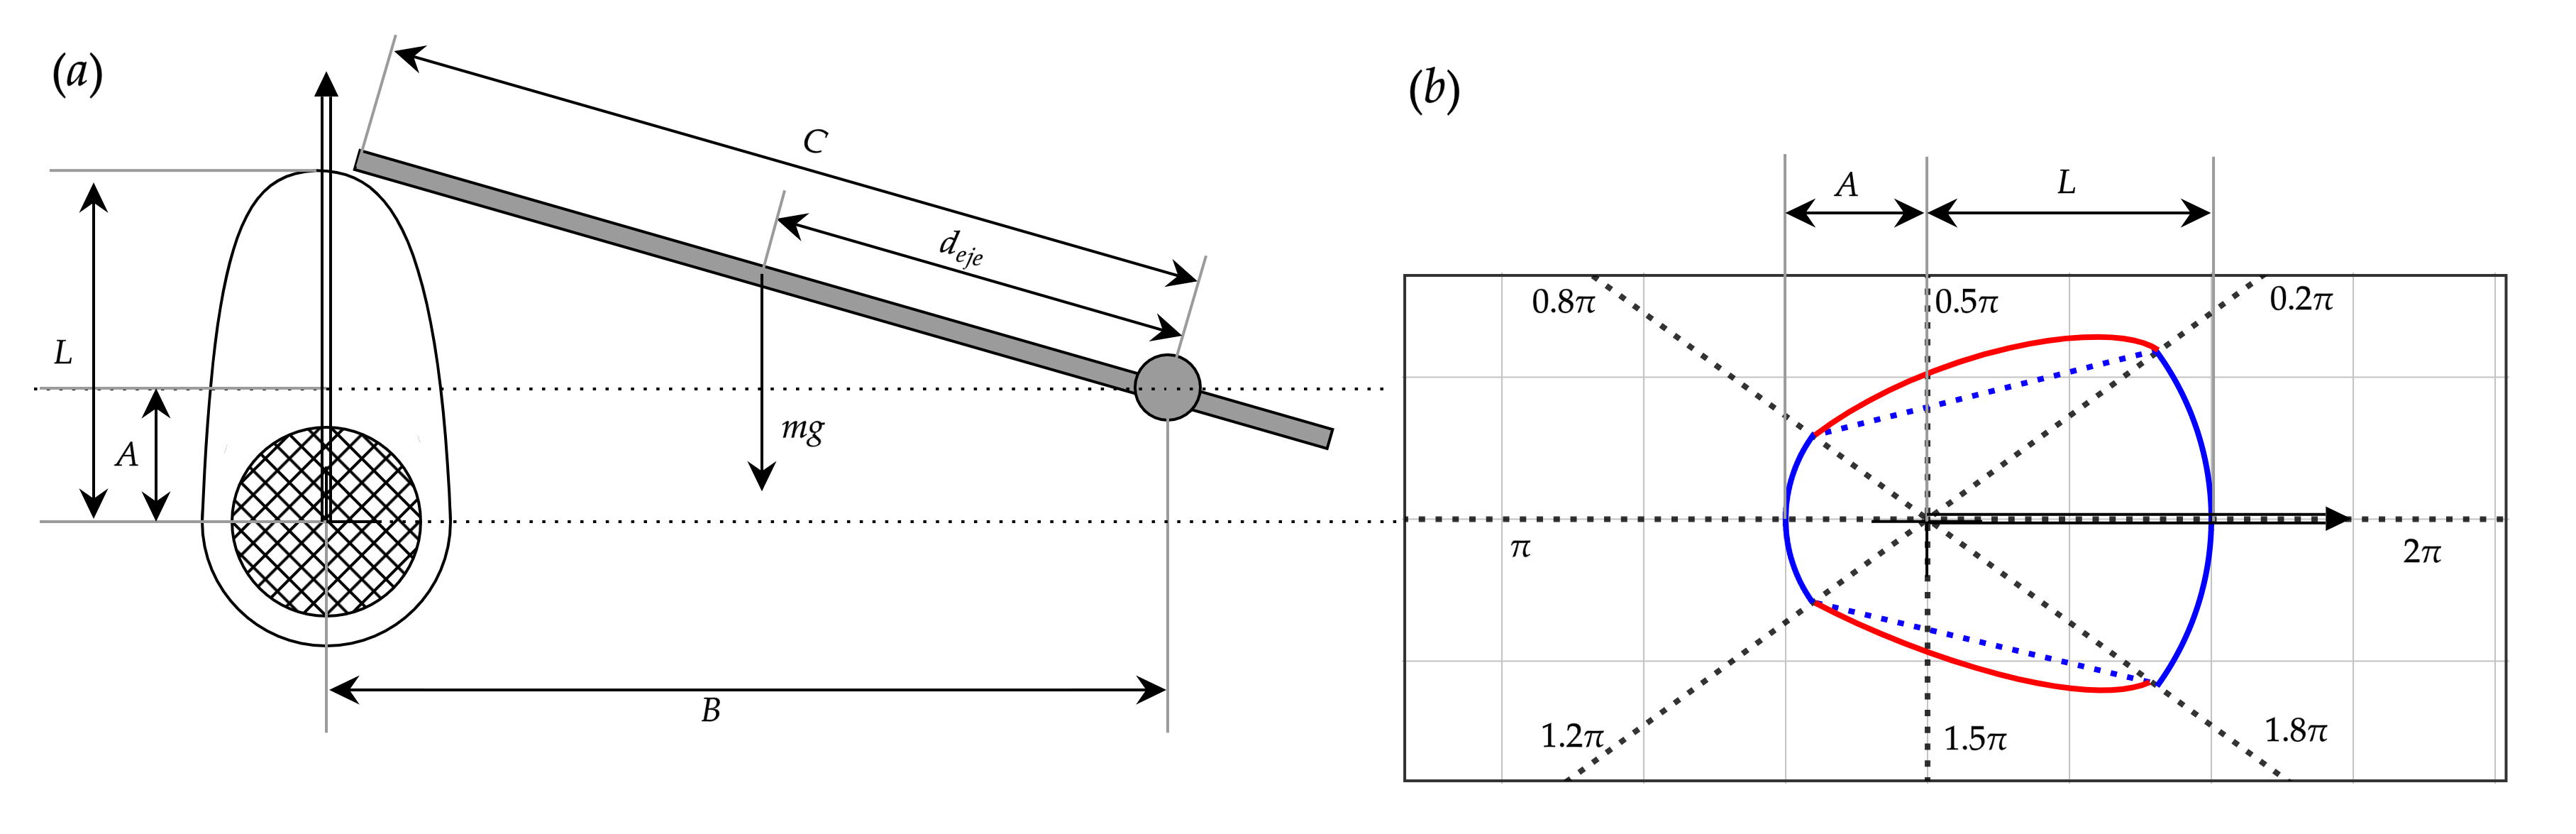
\includegraphics[width=1\textwidth]{chapter5/mecanismo compuerta.png}
	\caption[Mecanismo leva-seguidor]{(a) Diagrama de cuerpo libre de mecanismo leva-seguidor. (b) Dimensiones del disco de leva.}
	\begin{myflushcenter}
		Fuente: Elaboración propia.
	\end{myflushcenter}
	\label{fig:mecanismo compuerta}
\end{myfigure}

El diseño del disco de leva que se muestra en la Figura \ref{fig:mecanismo compuerta}-b corresponde al posicionamiento requerido (línea azul) y a un posicionamiento óptimo (línea roja). Dicho posicionamiento versus el ángulo de giro se muestra en la Figura \ref{fig:mecanismo compuerta leva posicionamiento}. 

\begin{myfigure}[H]
	\footnotesize\centering
	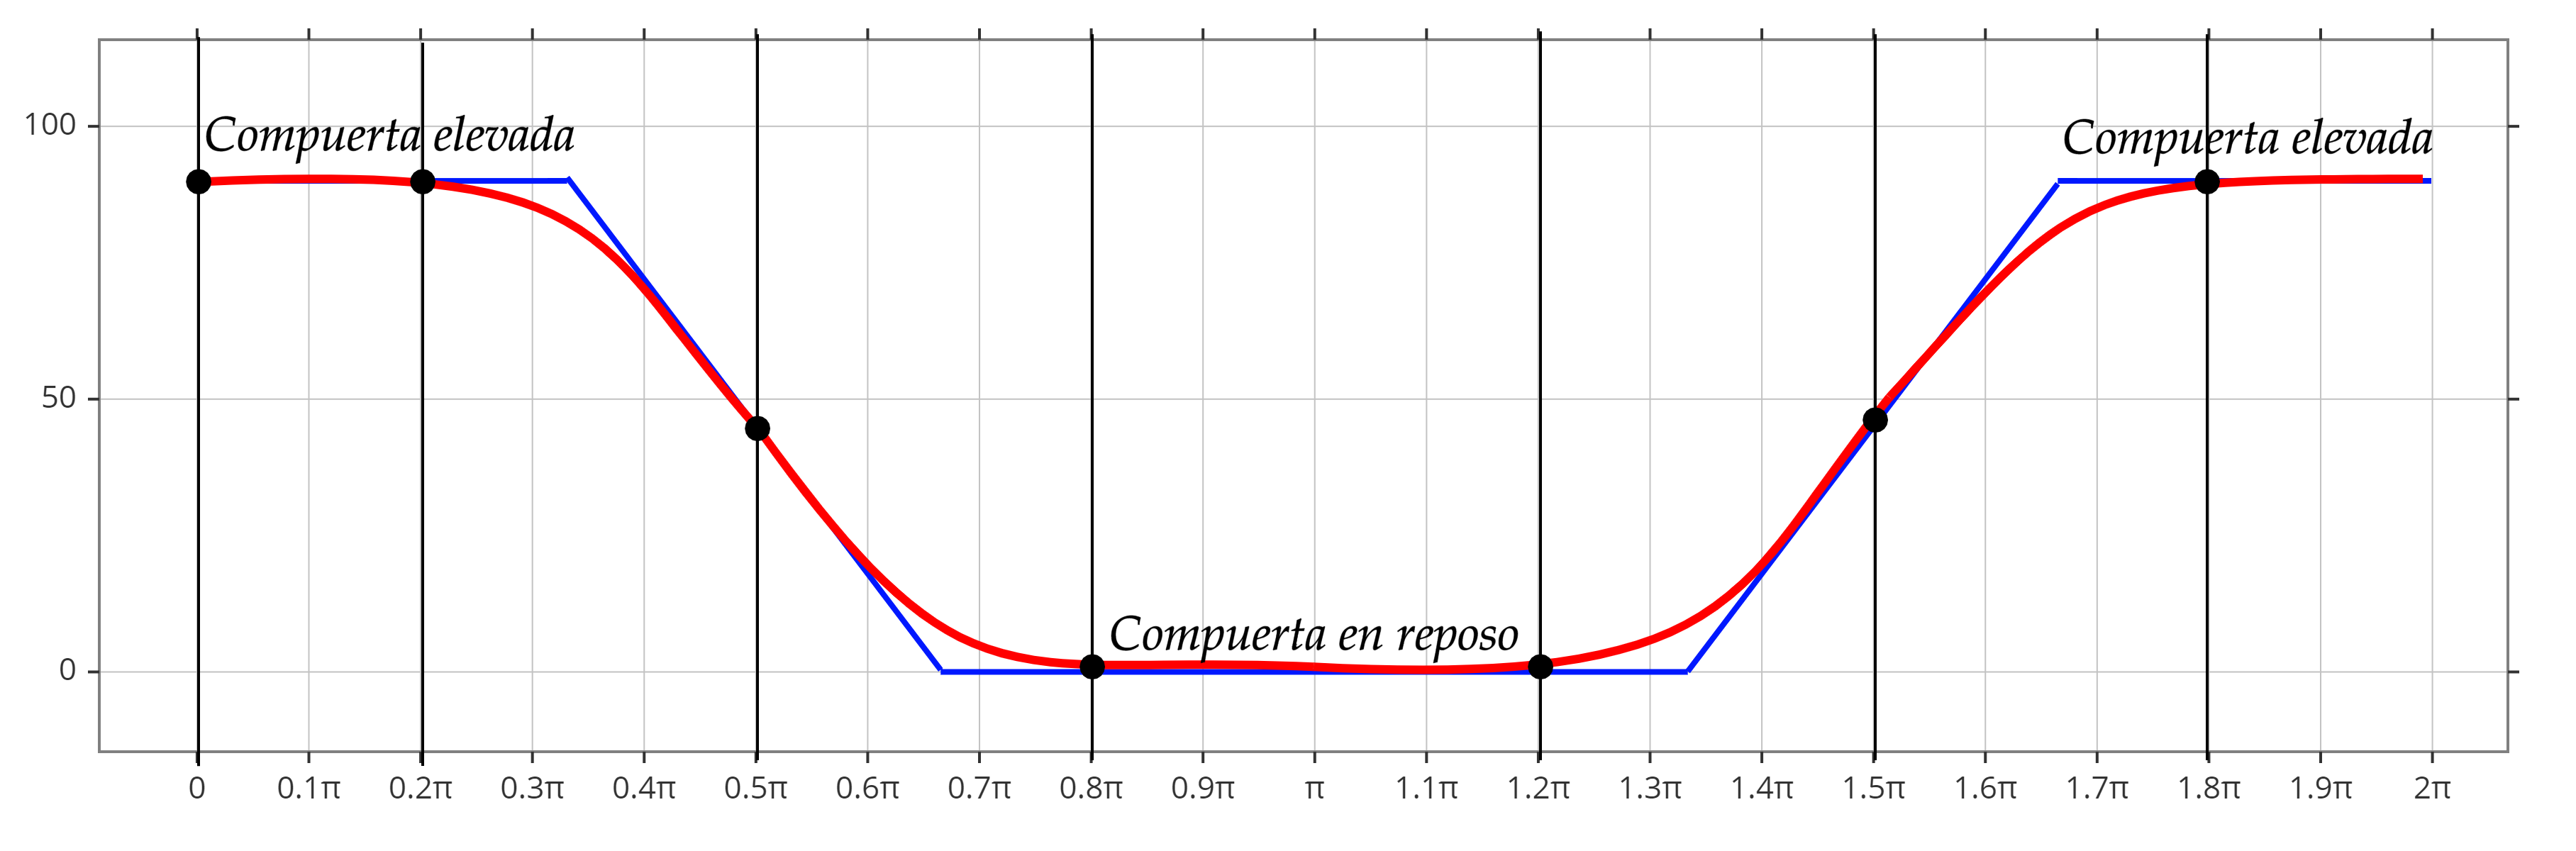
\includegraphics[width=1\textwidth]{chapter5/mecanismo compuerta leva posicionamiento.png}
	\caption{Engranajes del mecanismo de compuertas}
	\begin{myflushcenter}
		Fuente: Elaboración propia.
	\end{myflushcenter}
	\label{fig:mecanismo compuerta leva posicionamiento}
\end{myfigure}

%% NUEVO SECCION X.X.X.
\subsection{Cálculo de torque sobre la compuerta}

El torque necesario para abrir y cerrar la compuerta se aplica sobre el eje de la mima. La parte más alejada del disco de leva es la que levanta la compuerta. En la Figura \ref{fig:dlc leva compuerta}, la fuerza $N$ representa la normal que se aplica debido al peso de la compuerta cuando se abre en giro horario. Además, donde: [$R_x$, $R_y$] son reacciones en un determinado punto, en este caso sobre el eje del disco de leva y de la compuerta, respectivamente; [$C$, $d_{eje}$, $L$ y $A$] son distancias; y [$mg$ y $N$] son fuerzas a la que están sometidas las cuerpos.

\begin{myfigure}[H]
	\footnotesize\centering
	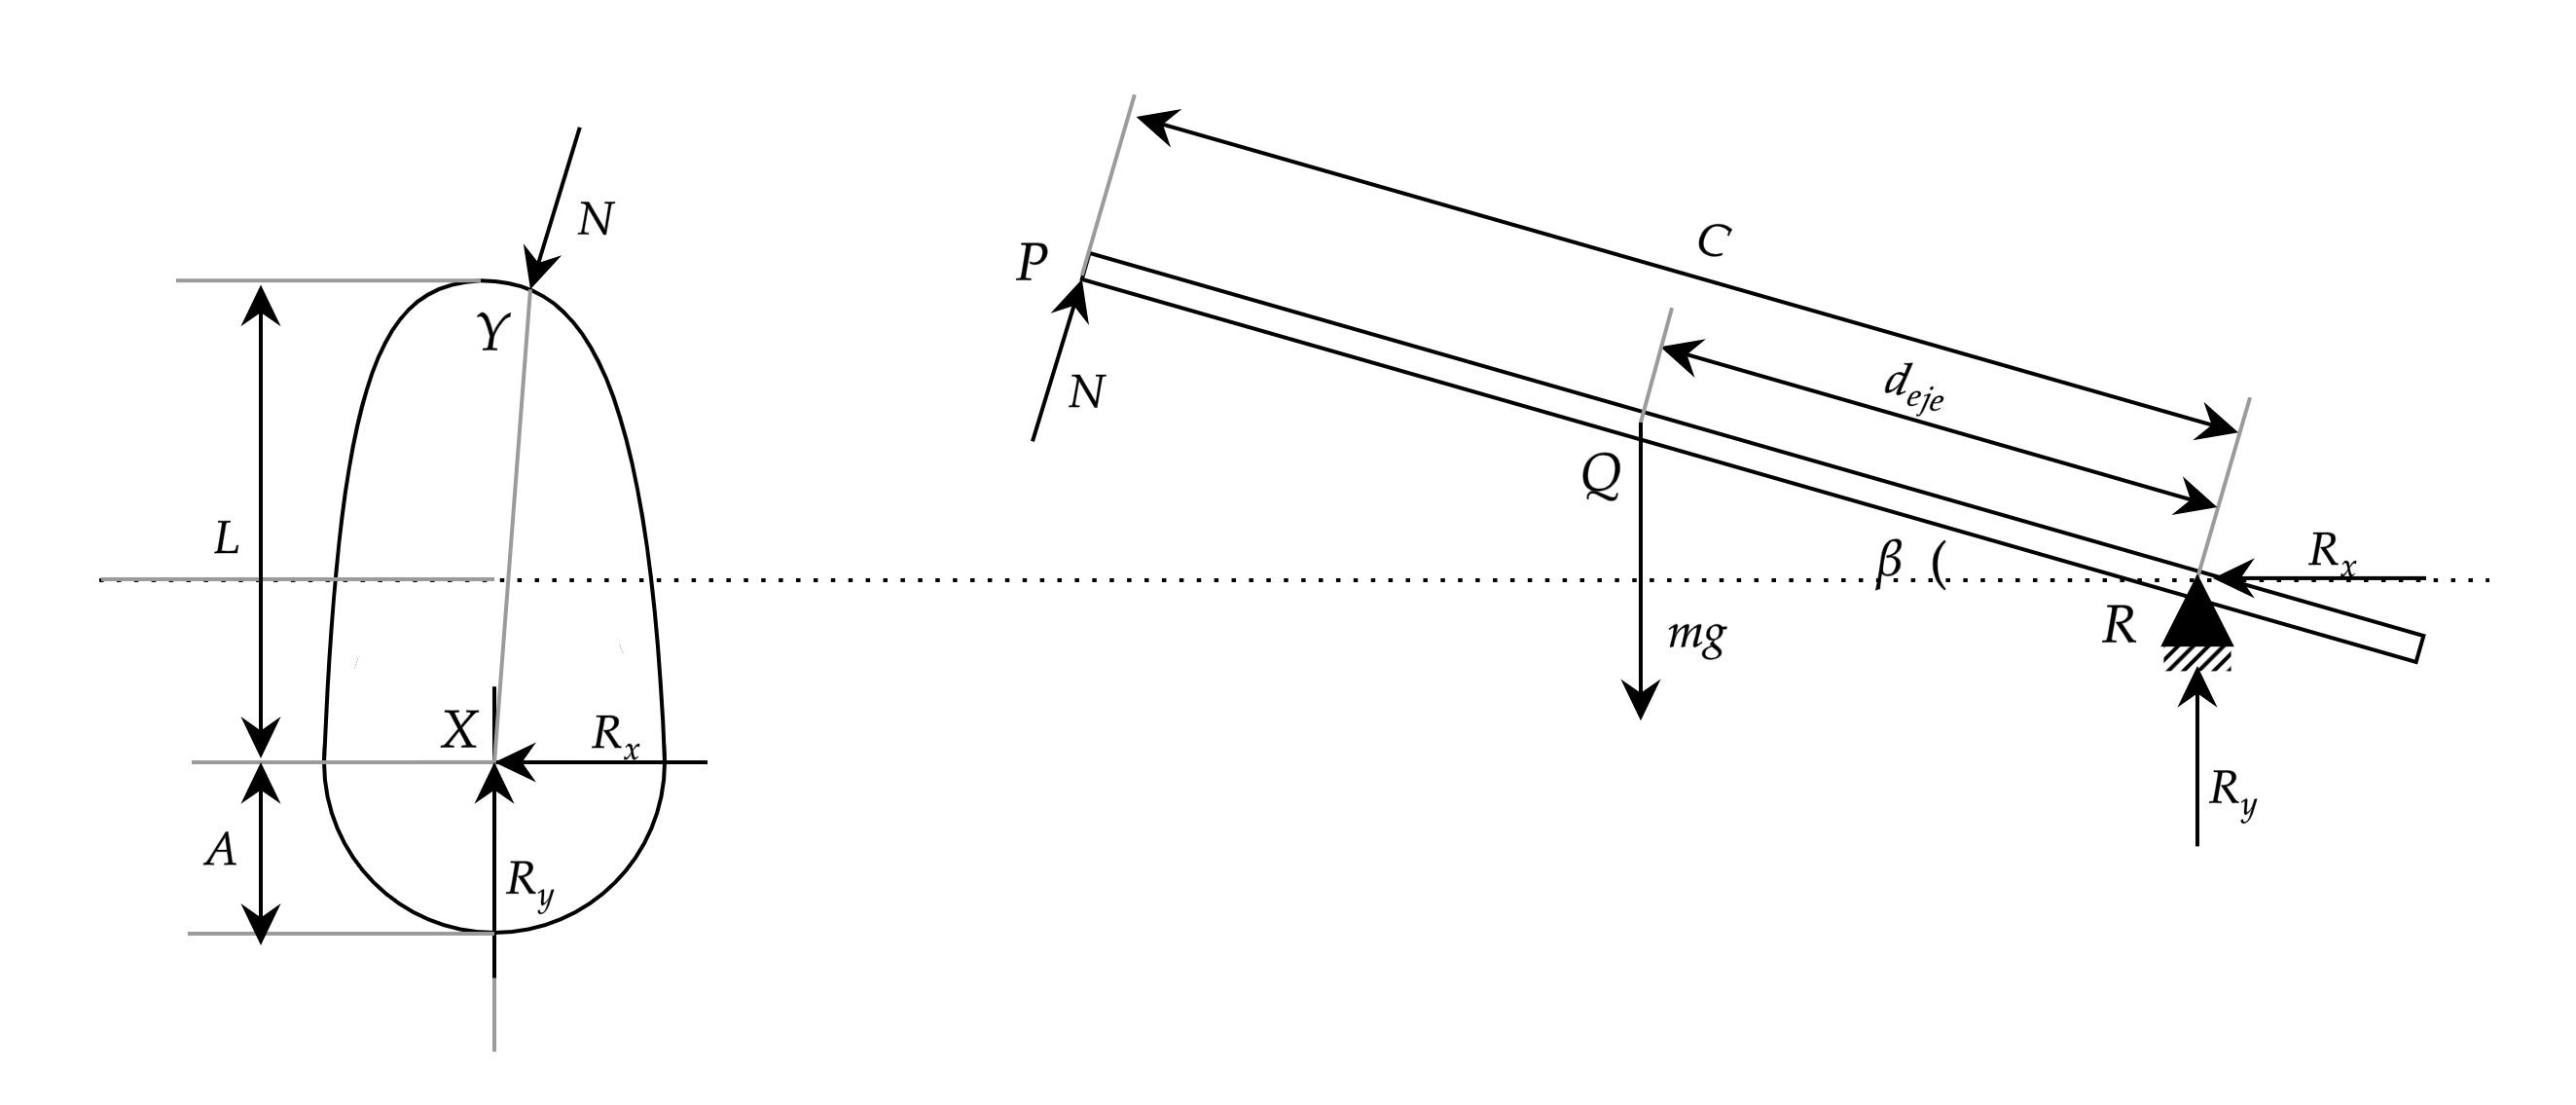
\includegraphics[width=1\textwidth]{chapter5/dlc leva compuerta.png}
	\caption[Diagrama de cuerpo libre del mecanismo de la compuerta]{(a) DLC del disco de leva. (b) DLC de la compuerta.}
	\begin{myflushcenter}
		Fuente: Elaboración propia.
	\end{myflushcenter}
	\label{fig:dlc leva compuerta}
\end{myfigure}

Para hallar el valor de la fuerza $N$, en el DLC de la compuerta (Figura \ref{fig:dlc leva compuerta}-b) se suma los momentos en el punto $R$ como se expone en la Ecuación \ref{eq:calculo fuerza normal}.	

\begin{myequation}\label{eq:calculo fuerza normal}
	\begin{split}
		\sum_{}^{}M_{R}&=m_{compuerta}*g*cos(\beta)*d_{eje}-2*N*d_{eje}=0 \\
		N&=\frac{m_{compuerta}*g*cos(\beta)}{2}			
	\end{split}		
\end{myequation}

Luego, analizamos realizamos la sumatoria de momentos en el punto $X$ en el DLC del disco de leva que se muestra en la Figura \ref{fig:diagrama de cuerpo libre del mecanismo de la leva}. 

\begin{myfigure}[H]
	\footnotesize\centering
	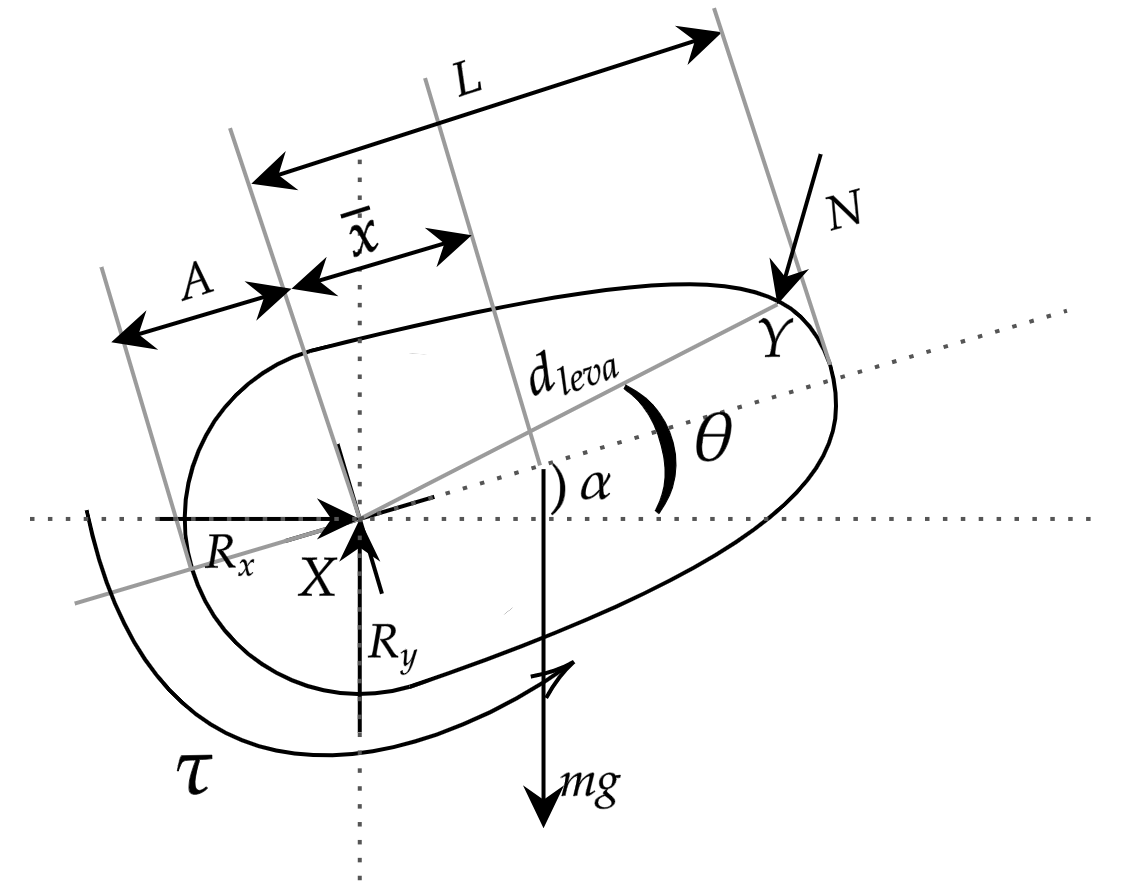
\includegraphics[width=0.45\textwidth]{chapter5/dlc leva.png}
	\caption{Diagrama de cuerpo libre del mecanismo de la leva}
	\begin{myflushcenter}
		Fuente: Elaboración propia.
	\end{myflushcenter}
	\label{fig:diagrama de cuerpo libre del mecanismo de la leva}
\end{myfigure}

Luego, se reemplaza el valor de $N$ en la sumatoria de momentos en el punto $X$, del DLC del disco de leva, y se obtiene el torque máximo ($\overrightarrow{\tau_{max}}$) como se muestra en la Ecuación \ref{eq:calculo de torque máximo}.

\begin{myequation}\label{eq:calculo de torque máximo}
	\begin{split}
		\sum_{}^{}M_{X}&=-m_{leva}*g*\bar{x}*cos(\alpha)+\tau-N*d_{leva}*(cos(\beta)cos(\theta)-sin(\beta)sin(\theta))=0 \\
		\tau_{max}&=m_{leva}*g*\bar{x}+N*d_{leva} \\
	\end{split}		
\end{myequation}

Dónde: $\bar{x}$ es el centro de gravedad, asumiendo material uniforme, $d_{leva}$ es la distancia del punto de apoyo $X$ al punto de contacto con la compuerta $Y$, $\theta$ es el ángulo que forma el punto de contacto respecto al eje $x$, $\alpha$ es el ángulo que se forma del eje $x$ al eje de simetría de la leva. Conocer el torque máximo ($\tau_{max}$) delimita la selección de un motor a pasos a base del par de fuerza máximo generado.

\begin{myequation}\label{eq:calculo de centro de gravedad}
	\begin{split}
		\bar{x}&=(\frac{2*sin(0.2*\pi)*(L-A)}{\pi}+2*\frac{L*cos(0.2*\pi)-A*cos(\pi)}{3})/4 \\
		\bar{x}&=54.23 \\	
	\end{split}		
\end{myequation}

\begin{myequation}\label{eq:calculo de masa de leva}
	\begin{split}
		m_{leva}&=V_{L}*\rho_{L}=39111.24*7.8/1000 \quad\quad (AISI 306 - e_{L}=3mm) \\
		m_{leva}&=305.06g=0.305kg \\		
	\end{split}		
\end{myequation}

\begin{myequation}\label{eq:calculo de masa de compuerta}
	\begin{split}
		m_{compuerta}&=V_{c}*\rho_{c}=41400*7.8/1000 \quad\quad (AISI 306 - e_{L}=1mm) \\
		m_{compuerta}&=322.92g=0.323kg \\	
	\end{split}		
\end{myequation}

\begin{myequation}\label{eq:calculo de fuerza normal maxima}
	\begin{split}
		N_{max}&=\frac{m_{c}*g}{2} \quad\quad (\beta=0^{\circ}) \\
		N_{max}&=\frac{0.323*9.8}{2}=1.579 \\		
	\end{split}		
\end{myequation}

Reemplazando los valores de las Ecuaciones \ref{eq:calculo de centro de gravedad}, \ref{eq:calculo de masa de leva}, \ref{eq:calculo de masa de compuerta} y \ref{eq:calculo de fuerza normal maxima} en la Ecuación \ref{eq:calculo de torque máximo} se obtiene el valor del torque máximo que es el mismo valor del par mínimo de fuerzas necesarias para seleccionar el motor a pasos. En la Ecuación \ref{eq:calculo de torque maximo 2} se calcula el valor del par de fuerzas.

\begin{myequation}\label{eq:calculo de torque maximo 2}
	\begin{split}
		\tau_{max}&=0.305*9.81*0.054+0.12*0.322*9.81/2 \\
		\tau_{max}&=1.86 \quad Nm \\
	\end{split}		
\end{myequation}

%	\begin{myequation}\label{eq:calculo de torque máximo}
%		\begin{split}
%			\overrightarrow{\tau_{X}}&=N*sin(\beta)*L \\
%			\overrightarrow{\tau_{X}}&=\frac{m*g*cos(\beta)}{2}*sin(\beta)*L \\
%			\overrightarrow{\tau_{X}}&=m*g*L*\frac{sin(2\beta)}{2} \\
%			\overrightarrow{\tau_{X_{max}}}&=\frac{m*g*L}{2} \quad (\beta=45^\circ) \\
%		\end{split}		
%	\end{myequation}

%	\item \textbf{Cálculo de velocidad de giro de la compuerta}

%	\textcolor{blue}{[BORRADOR] Falta pasar a limpio los cálculos [/BORRADOR]}

%	\begin{myfigure}[H]
%		\footnotesize\centering
%		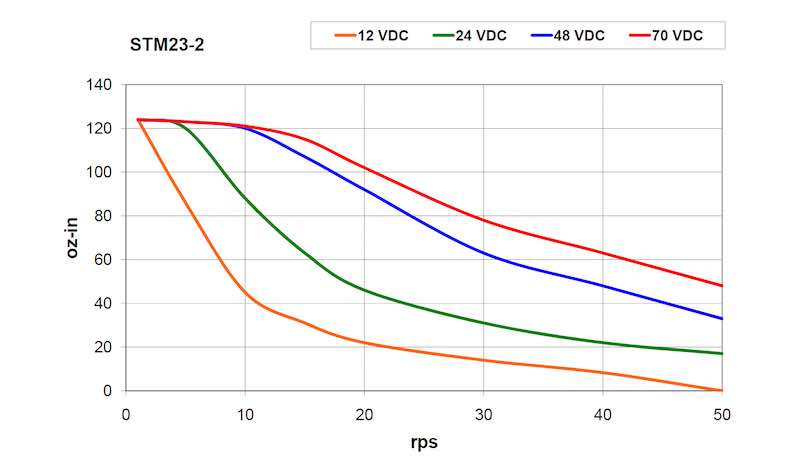
\includegraphics[width=1\textwidth]{chapter5/torque necesario.png}
%		\caption{Curva de torque necesario}
%		\begin{myflushcenter}
%			Fuente: Elaboración propia.
%		\end{myflushcenter}
%		\label{fig:curva de torque necesario}
%	\end{myfigure}

%	\textcolor{blue}{[BORRADOR] La velocidad de compuertas debe ir acorde a la distancia entre una trucha y la siguiente a esta.  Explicar velocidad RPM necesarias y explicar las ecuaciones siguientes [/BORRADOR]}

%	\begin{myequation}\label{eq:calculo de rpms}
%		\begin{split}
%			RPM_{necesarias}&=1 \\
%		\end{split}		
%	\end{myequation}

%% NUEVO SECCION X.X.X.
\subsection{Selección de motores a paso}
	
La selección de los motores a pasos depende se da acorde a los cálculos en las subsecciones anteriores, existe una gran variedad en cuanto a este tipo de dispositivos en el mercado internacional.En la Tabla \ref{tab:tabla comparativa de motores a pasos} se muestra una comparación técnica entre tres motores a pasos que cumplen los requisitos mínimos.	 

\begin{mytable}[H]
	\footnotesize\centering
	\caption{Tabla comparativa de motores a pasos.}
	\label{tab:tabla comparativa de motores a pasos}
	\begin{tabular}{l|c|c|c|c|}
		\cline{2-5}
		\multicolumn{1}{c|}{\textbf{}} & \textbf{\begin{tabular}[c]{@{}c@{}}Requisitos\\ mínimos\end{tabular}} &
		\begin{minipage}{\mythirdmaxsizeofcontenttable}\begin{myflushcenterinsidetable}
			\textbf{57J1880-450}
		\end{myflushcenterinsidetable}\end{minipage} &		
		\begin{minipage}{\mythirdmaxsizeofcontenttable}\begin{myflushcenterinsidetable}
			\textbf{Nema 34}
		\end{myflushcenterinsidetable}\end{minipage} &	
		\begin{minipage}{\mythirdmaxsizeofcontenttable}\begin{myflushcenterinsidetable}
			\textbf{ZL57HS09}
		\end{myflushcenterinsidetable}\end{minipage} \\ \hline
		\multicolumn{1}{|l|}{\textbf{Figura}}     & -                                                                     
		&
		\begin{minipage}{\mythirdmaxsizeofcontenttable}
			\centering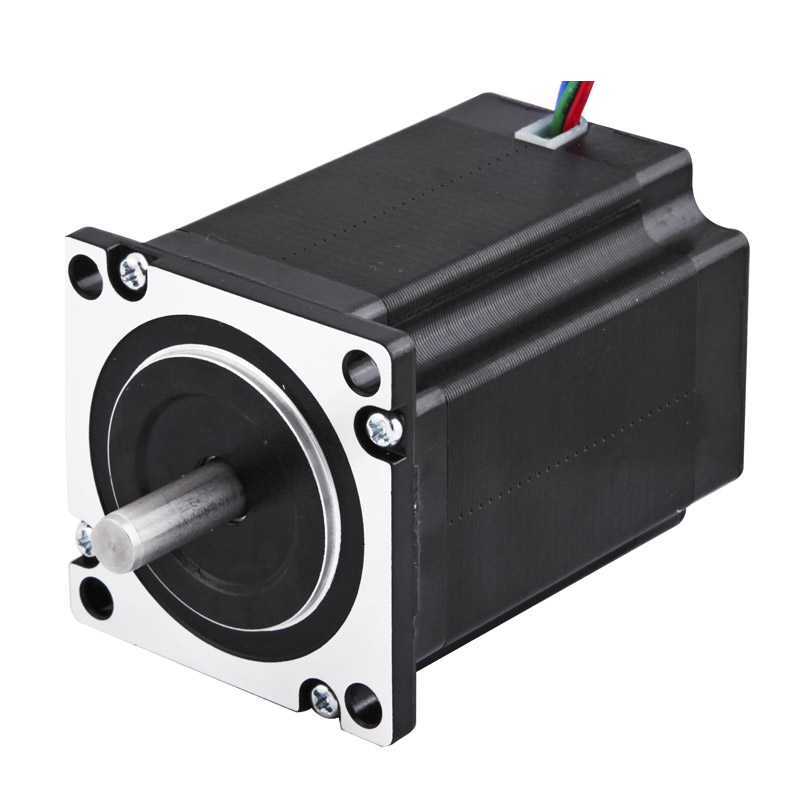
\includegraphics[width=\mythirdmaxsizeimageinsidetable]{chapter5/tablas comparativas/motor a pasos 1.png} \\ 
			%\begin{myflushcenter}
			%	{\footnotesize Nombre imagen}
			%\end{myflushcenter}
		\end{minipage} 
		&
		\begin{minipage}{\mythirdmaxsizeofcontenttable}
			\centering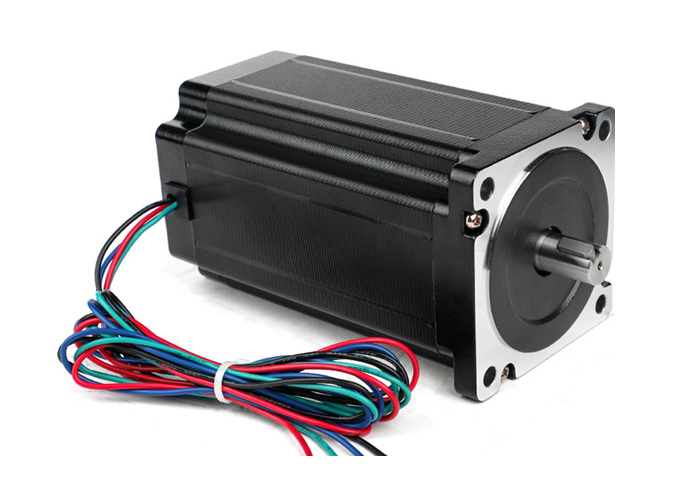
\includegraphics[width=\mythirdmaxsizeimageinsidetable]{chapter5/tablas comparativas/motor a pasos 2.png} \\ 
			%\begin{myflushcenter}
			%	{\footnotesize Nombre imagen}
			%\end{myflushcenter}
		\end{minipage} 
		&
		\begin{minipage}{\mythirdmaxsizeofcontenttable}
			\centering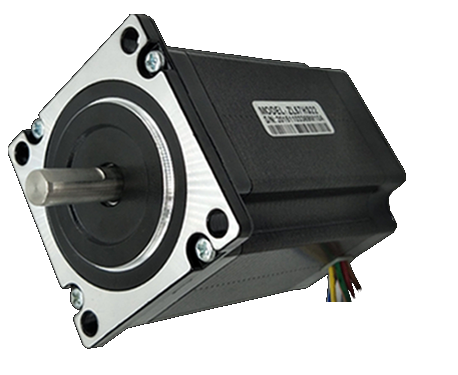
\includegraphics[width=\mythirdmaxsizeimageinsidetable]{chapter5/tablas comparativas/motor a pasos 3.png} \\ 
			%\begin{myflushcenter}
			%	{\footnotesize Nombre imagen}
			%\end{myflushcenter}
		\end{minipage} 
		\\ \hline
		\multicolumn{1}{|l|}{\textbf{Fabricante}} & - &
		\begin{minipage}{\mythirdmaxsizeofcontenttable}\begin{myflushcenterinsidetable}
			JMC
		\end{myflushcenterinsidetable}\end{minipage} &
		\begin{minipage}{\mythirdmaxsizeofcontenttable}\begin{myflushcenterinsidetable}
			Jingbang
		\end{myflushcenterinsidetable}\end{minipage} & 
		\begin{minipage}{\mythirdmaxsizeofcontenttable}\begin{myflushcenterinsidetable}
			IM42EL-RS
		\end{myflushcenterinsidetable}\end{minipage} \\ \hline
		\multicolumn{1}{|l|}{\textbf{Dimensiones ($mm.$)}}& - & 57x57x80 & 86x86x67 & 50x50x100 \\ \hline
		\multicolumn{1}{|l|}{\textbf{Torque máximo ($Nm$)}}& 1.86 & 2.2 & 2.4 & 2.8 \\ \hline
		\multicolumn{1}{|l|}{\textbf{Diámetro de eje ($mm.$)}}& - & 8 & [14; 16] & 8 \\ \hline
		\multicolumn{1}{|l|}{\textbf{Peso ($kg$)}}& $<$2 & 1.2 & - & 1.5 \\ \hline
		\multicolumn{1}{|l|}{\textbf{Voltaje de alimentación ($V$)}}& 24 & Driver (24/48) & Driver (24/48) & 24 \\ \hline
		\multicolumn{1}{|l|}{\textbf{Corriente de fase ($A$)}}& - & 4 & 2 & 5 \\ \hline
		\multicolumn{1}{|l|}{\textbf{Temperatura operativa (°$C$)}}& - & - & [-20;60] & - \\ \hline
		\multicolumn{1}{|l|}{\textbf{Inductancia de fase ($mH$)}}& - & 1.8 & $\approx$9 & 2.0 \\ \hline
		\multicolumn{1}{|l|}{\textbf{Precio ($S/$)}}& - & 78.98 & 53.85 & 150.24 \\ \hline
	\end{tabular}
	\begin{myflushcenteraftertable}	
		Fuente: Imágenes de dominio público y elaboración propia. Hoja de datos técnica (\textit{Datasheet}) en el Anexo. \\
		Tasa de cambio de USD a PEN: S/ 3.59.
	\end{myflushcenteraftertable}
\end{mytable}

El modelo de motor a pasos del fabricante Jingbang, basado en Nema34 S/C, posee un torque de 2.4 que si bien es inferior a los 2.8 que ofrece el modelo ZL57HS09, este último triplica el precio del primero e es incluso menor que el modelo 57J1880-450, por lo que la relación $torque/precio$ es mayor en el modelo escogido.

%% NUEVO SECCION X.X.X.
\subsection{Selección de driver de motor a pasos}
	
Debido a las características únicas de cada servomotor, los fabricantes de cada marca recomiendan utilizar los drivers dedicados para sus componentes. Este trabajo no será la excepción, por lo que en la Tabla \ref{tab:driver del motor a pasos escogido} se muestra el driver del motor escogido en la subsección anterior.

\begin{mytable}[H]
	\footnotesize\centering
	\caption{Tabla comparativa de motores a pasos.}
	\label{tab:driver del motor a pasos escogido}
	\begin{tabular}{l|c|}		
		\cline{2-2}
		\multicolumn{1}{c|}{\textbf{}}            & \textbf{DM860H}  \\ \hline
		\multicolumn{1}{|l|}{\textbf{Figura}}     & 
		\begin{minipage}{\mythirdmaxsizeofcontenttable}
			\centering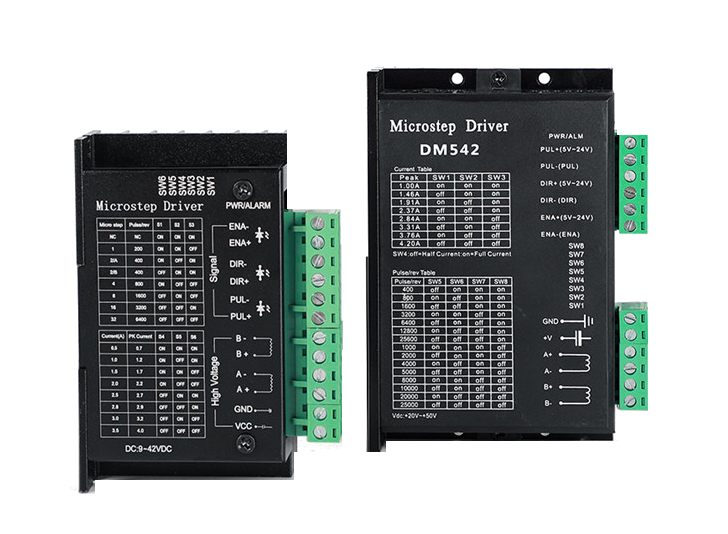
\includegraphics[width=\mythirdmaxsizeimageinsidetable]{chapter5/driver del motor a pasos escogido.png} \\ 
		\end{minipage} \\ \hline		
		\multicolumn{1}{|l|}{\textbf{Fabricante }} & Jingbang  \\ \hline
		\multicolumn{1}{|l|}{\textbf{Modelo de driver }} & 	Nema 34  \\ \hline
		\multicolumn{1}{|l|}{\textbf{Pico de corriente ($A$) }} & 7.2 \\ \hline
		\multicolumn{1}{|l|}{\textbf{Señal digital ($V$) }} & 5/ 24 \\ \hline
		\multicolumn{1}{|l|}{\textbf{Voltaje de alimentación ($V$) }} & [24; 110] \\ \hline
		\multicolumn{1}{|l|}{\textbf{Precio ($S/$)}} & 71.8  \\ \hline
	\end{tabular}
	\begin{myflushcenteraftertable}	
		Fuente: Imágenes de dominio público y elaboración propia. Hoja de datos técnica (\textit{Datasheet}) en el Anexo. \\
		Tasa de cambio de USD a PEN: S/ 3.59.
	\end{myflushcenteraftertable}
\end{mytable}
	
%% NUEVO SECCION X.X.X.
%% \subsection{Diseño de juego de compuertas programables}
%% Descripción.

%% NUEVO SUBSECCION X.X.X.
\section{Diseño de subsistema de traslado de truchas}

Las tuberías del sistema tienen como propósito abastecer de un flujo de agua constante a la máquina mientras está en funcionamiento. Cuatro canales de tuberías se abastecen de un flujo mediante este subsistema, accionado por bombas de agua y controlados por electroválvulas y sensores de caudal. Esto permite un correcto abastecimiento que no perjudique a las truchas. En las siguientes subsecciones se detalla el dimensionamiento de las tuberías, cálculo de caudales apropiados, selección de electroválvulas, su control asociado y selección de bombas de agua.

%% NUEVO SECCION X.X.X.
\subsection{Diseño de tuberías}
	
Las tuberías por las que las truchas transitarán en un solo sentido deben satisfacer los requerimientos mínimos técnicos: diámetro no menor al alto o ancho de una trucha. En el \textit{Estado del Arte}\footnote{Referencia de \cite{DiazVergara2020}.}, se observa que las truchas de 10 a 20 $cm.$ tienen un alto máximo de 60 a 90 $mm.$\footnote{Distancia máxima entre aleta superior e inferior más alejada del cuerpo. En truchas de 30 $cm.$ dicha distancia puede llegar hasta 135 $mm.$}

%% NUEVO SECCION X.X.X.
\subsection{Cálculo de caudales y selección de la bomba de agua}
	
En el diseño de las tuberías se toma en cuenta los siguientes parámetros: caudal necesario, viscosidad del fluido, presión operativa máxima, entre otros.\footnote{Extraído de \cite{INTECHGmbH2020}.} Se requiere un flujo laminar en el subsistema de procesamiento de imágenes, es decir, en la sección con tubo transparente en el que se captura fotogramas sobre las truchas en tránsito. Sin embargo, debido a los requerimientos del sistema en cuanto al diámetro de tuberías, se optará por un flujo de tipo turbulento pero horizontal\footnote{Flujo de agua dentro de una tubería que abarca toda la sección y genera pequeñas burbujas de aire.}. Entonces, para los valores de $D_{int}=3.5''=88.9 mm$ y $v=210 cm/s$ se calcula el número de Reynolds ($Re$) en la Ecuación \ref{eq:calculo de reynolds}.
	
\begin{myequation}\label{eq:calculo de reynolds}
	\begin{split}
		Re &= \frac{\rho*v*D_{int}}{\mu} \\
		Re &= \frac{999.7*2.1*0.0889}{0.001307} \\
		Re &= 142795.71 \approx 1.4x10^5
	\end{split}		
\end{myequation}

Donde: $\rho$ es la densidad del agua a 10 °C ($kg/m^3$), $v$ es la velocidad del fluido ($m/s$), $D_{int}$ es el diámetro interior de la tubería escogida ($m$), $\mu$ es la viscosidad dinámica del fluido a 10° C ($N*s/m^2$) y el número de Reynolds es adimensional. Luego, con $Re\approx1.4x10^5$ y sabiendo que la rugosidad de una tubería circular de PVC ($\varepsilon$) es $0.015 mm.$ podemos calcular el valor de rugosidad relativa ($\varepsilon/d=0.01687$) y el valor del coeficiente de rozamiento ($\lambda$) como se muestra en la Figura \ref{fig:diagrama de moody} empleando el diagrama de Moody.
	
\begin{myfigure}[H]
	\footnotesize\centering
	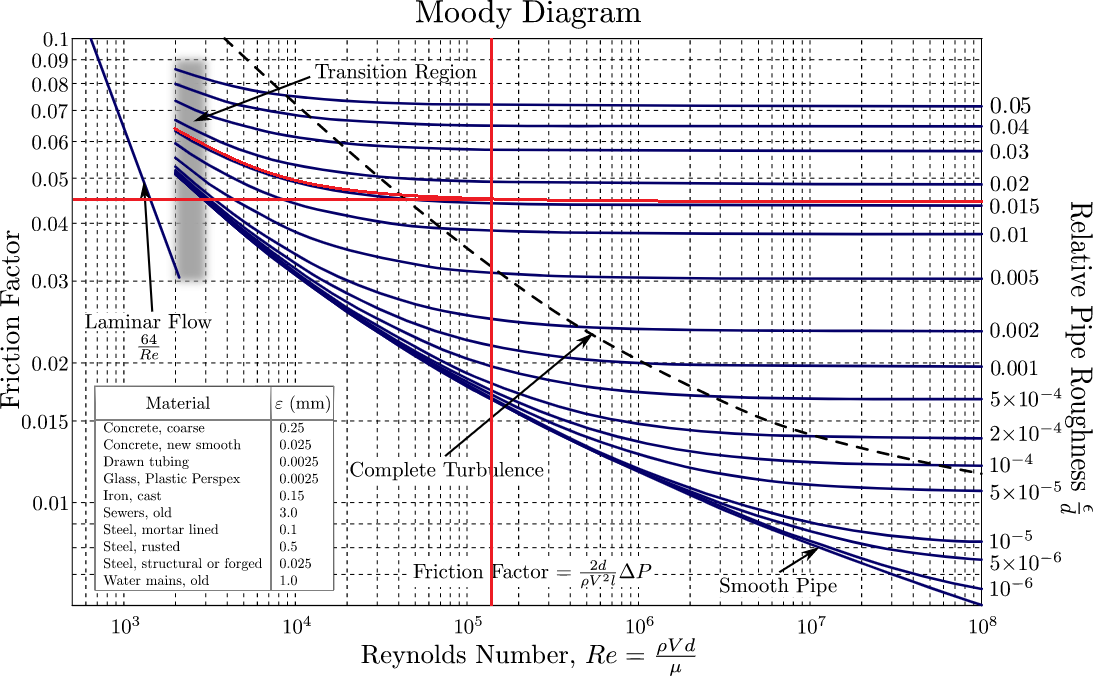
\includegraphics[width=1\textwidth]{chapter5/diagrama de moody.png}
	\caption{Calculo de coeficiente de rozamiento usando diagrama de Moody.}
	\begin{myflushcenter}
		Fuente: \cite{Janna2015}.
	\end{myflushcenter}
	\label{fig:diagrama de moody}
\end{myfigure}

Consecuentemente, el valor hallado para $\lambda$ es $\approx 0.046$. Sin embargo, para flujos turbulentos se emplea la ecuación de Colebrook–White, con la cual podemos hallarla con mayor precisión como se muestra en la Ecuación \ref{eq:calculo de coeficiente de fricción}.

\begin{myequation}\label{eq:calculo de coeficiente de fricción}
	\begin{split}
		\frac{1}{\sqrt{\lambda}} &= -2*log(\frac{2.51}{Re*\sqrt{\lambda}} + \frac{k}{3.71*d})
	\end{split}		
\end{myequation}

El valor de $\lambda$ es $0.0087$. Con este valor, podemos calcular la presión operativa necesaria para el sistema, que garantice el funcionamiento de la tubería como es esperado. El diagrama mostrado en la Figura \ref{fig:diagrama de tuberias} expone un recorrido horizontal del agua en el sistema, por lo que en la Ecuación \ref{eq:calculo de caudal} se calcula el caudal requerido a la salida.

\begin{myfigure}[H]
	\footnotesize\centering
	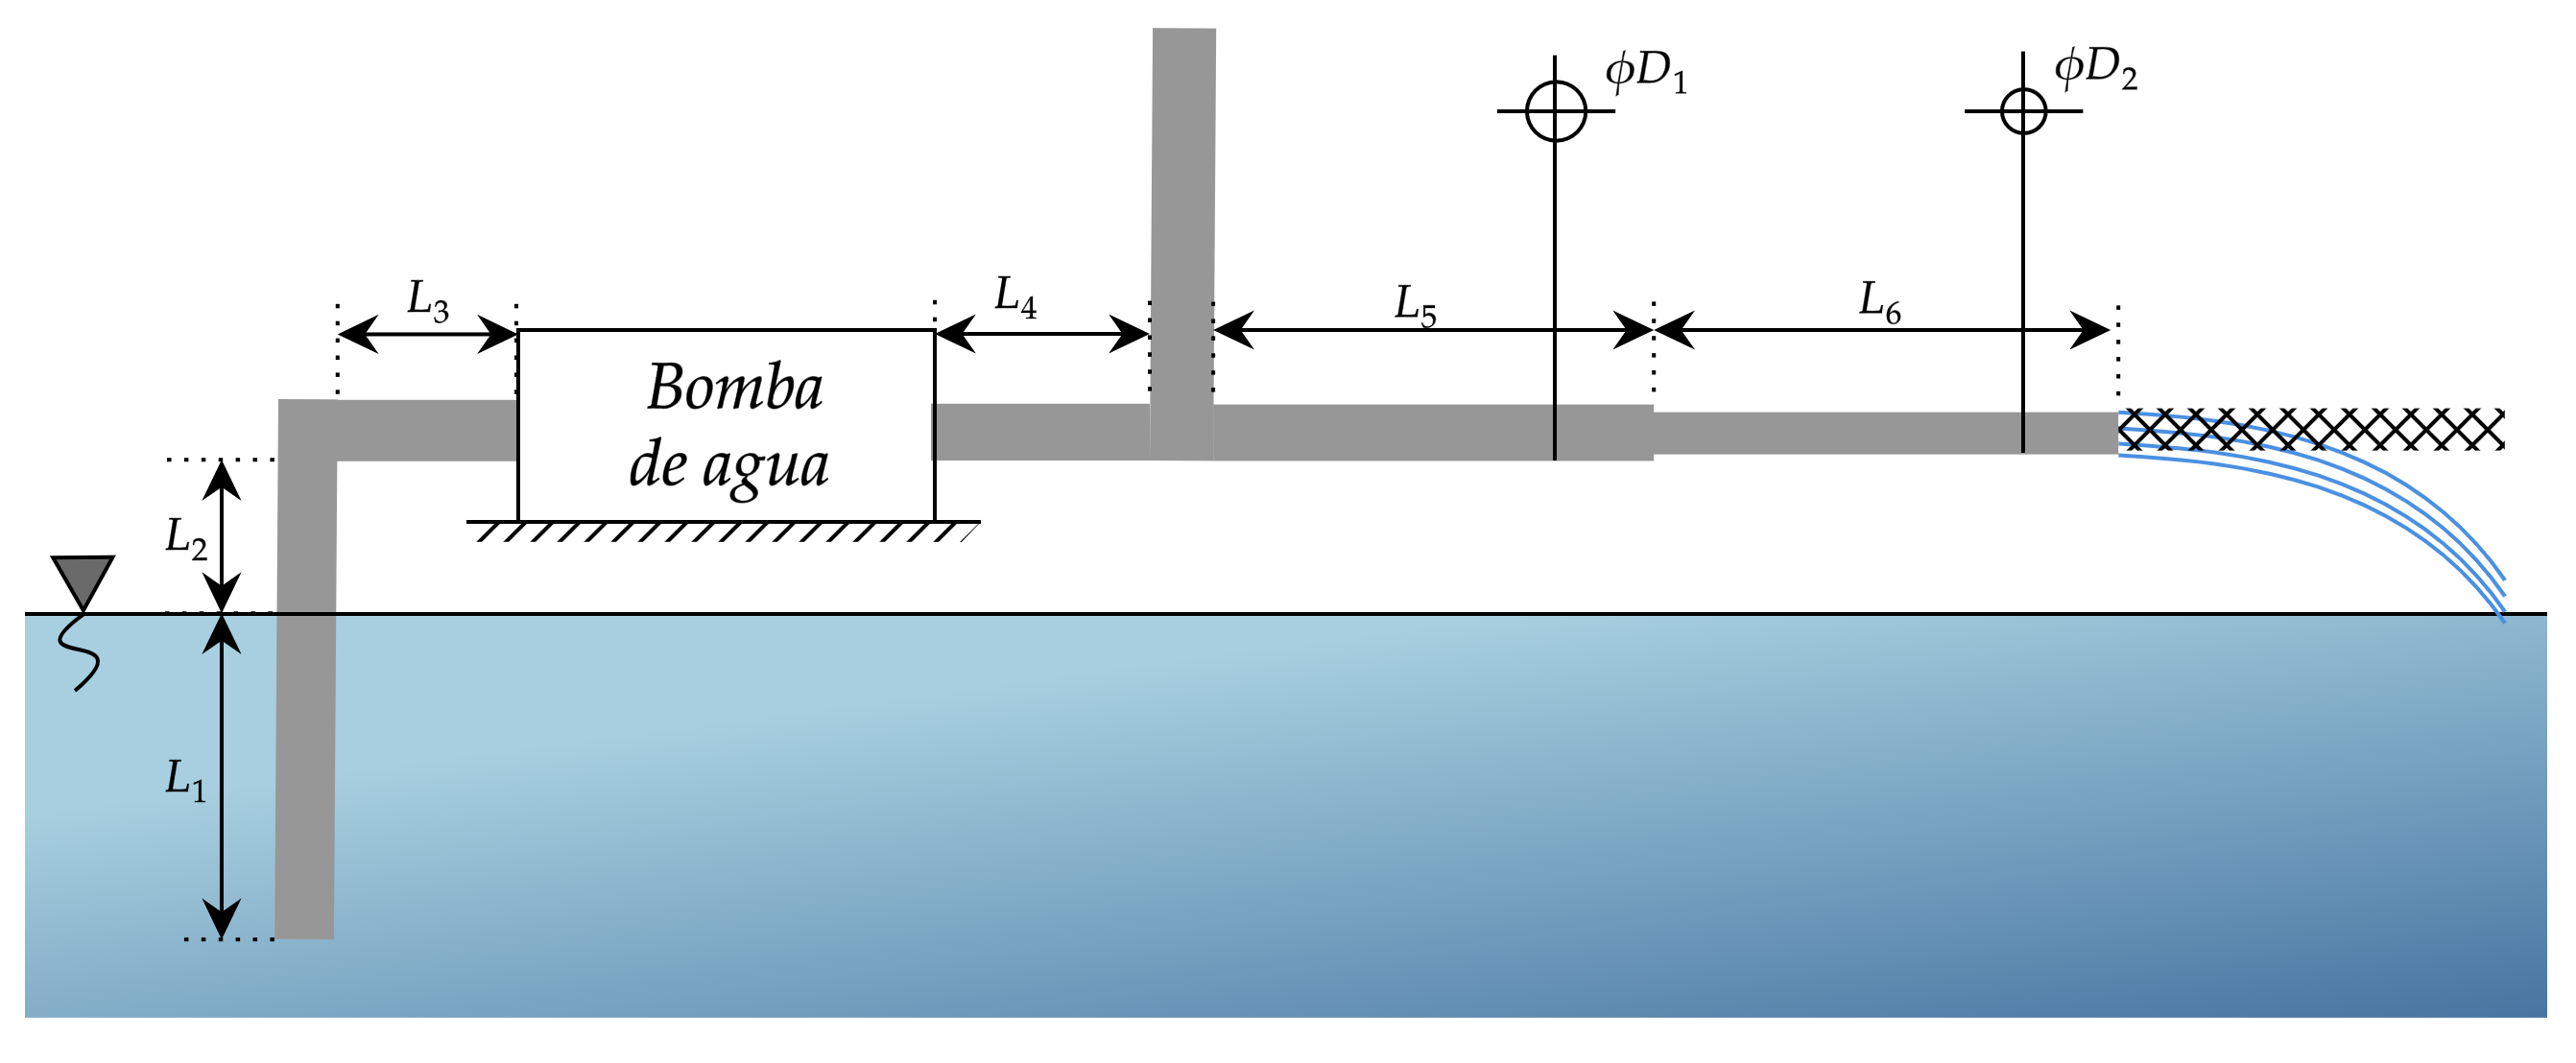
\includegraphics[width=1\textwidth]{chapter5/diagrama de tuberias.png}
	\caption{Diagrama de tuberías.}
	\begin{myflushcenter}
		Fuente: Elaboración propia.
	\end{myflushcenter}
	\label{fig:diagrama de tuberias}
\end{myfigure}

\begin{myequation}\label{eq:calculo de caudal}
	\begin{split}
		Q &= A*v \\
		Q &= \frac{\pi*0.0762^2}{4}*2.1 \\
		Q &= 0.00957 \; (m^3/s) = 13.064 \; (L/s) \\
		Q_{req} &= 15 \; (L/s)
	\end{split}		
\end{myequation}

Dónde: $Q$ es el caudal ($m^3/s$) que fluye sobre una tubería circular de área $A$ ($m^2$) a una velocidad $v$ ($m/s$). Luego, en la Ecuación \ref{eq:calculo de pérdida de presion} se calcula la pérdida de carga en la tubería horizontal.

\begin{myequation}\label{eq:calculo de pérdida de presion}
	\begin{split}
		h_{L} &= h_{ma}+ h_{me} \\
		h_{L} &= f\frac{l}{D}\frac{v^2}{2g} + K_{L_{r}}\frac{v^2}{2g} + K_{L_{u}}\frac{v^2}{2g}\\
		h_{L} &= f\frac{l}{D}\frac{v^2}{2g} + K_{L_{r}}\frac{v^2}{2g} + 0.42(1-\frac{D_{2}}{D_{1}})\frac{v^2}{2g}\\
		h_{L} &= 0.0087\frac{2}{0.089}\frac{2.1^2}{2(9.81)} + 0.08\frac{2.1^2}{2(9.81)} + 0.42(1-\frac{0.089}{0.076})\frac{2.1^2}{2(9.81)}\\
		h_{L} &= 0.045 \; (m)
	\end{split}		
\end{myequation}

Dónde: $h_{L}$ es la pérdida de carga ($m$), $h_{ma}$ es la representación de las pérdidas de carga mayores, $h_{me}$ son las menores, $f$ es el factor de fricción , $l$ es la distancia horizontal ($m$), $D$ es el diámetro interior de la tubería ($m$), $v$ es la velocidad media del líquido ($m/s$), $g$ es la fuerza gravitacional ($m/s^2$) y $K_{L_{r}}$ es el coeficiente de pérdida por unión y $K_{L_{r}}$ es correspondiente a la reducción de diámetro. Entonces, la presión operativa puede ser calculada mediante la ecuación de Darcy–Weisbach como se muestra en la Ecuación \ref{eq:calculo de presion operativa}.

\begin{myequation}\label{eq:calculo de presion operativa}
	\begin{split}
		p_{b}-p_{s}&=\rho g(z_{2}-z{1})+\rho g h_{L} \\
		p_{b}-101.32 &= 441.31 \\
		p_{b}&= 542.63 \; (kPa) \\
		p_{b}&\approx 550 \; (kPa) \approx 80 \; (psi) \\			
	\end{split}		
\end{myequation}

Al momento de seleccionar bombas de agua, en la industria se suele usar un valor dependiente de la presión operativa: la altura de succión positiva neta ($NPSH$) que se define y calcula en la Ecuación \ref{eq:calculo de npsh}.

\begin{myequation}\label{eq:calculo de npsh}
	\begin{split}
		h_{NPSH} &= 2.31*\frac{p_{b}}{SG} \\
		h_{NPSH} &= 2.31*\frac{80}{9.804} \\
		h_{NPSH} &= 18.85 \; (m) \\
		h_{NPSH_{req}} &\approx 20 \; (m) \approx 65 \; (ft) \\
	\end{split}		
\end{myequation}

Dónde: $p_{b}$ es la presión operativa mínima requerida de la bomba de agua ($kPa$), $SG$ es el peso específico ($\gamma$)($kN/m^3$) del agua a 10 °C. Finalmente, se ingresa los requisitos mencionados al seleccionador de bombas de agua online de la empresa Hidrostal\footnote{Sitio web de seleccionador de bombas de agua: \href{https://www.hidrostal.com/pumpselector/}{https://www.hidrostal.com/pumpselector/}. Los grandes fabricantes suelen tener programas online para facilitar la selección de entre cientos de modelos.}: la empresa retorna un modelo de bomba de agua D03R-EHN con un motor DEYS4 que cumple con la certificación ISO 9906:2012 Grado 3B\footnote{Más detalles en \href{https://www.iso.org/standard/41202.html}{https://www.iso.org/standard/41202.html}.}. Además, mencionar que el consumo de potencia es de 2.1 $kW$, trabaja a una velocidad de 1435 $rpm$ con una eficiencia del $69.8\%$ y que puede variar el caudal de 10 a 24 $L/s$.\footnote{Hoja de datos (Datasheet) en el Anexo.}

%% NUEVO SECCION X.X.X.
\subsection{Selección de las electroválvulas}

Los valores límites que se tendrían que controlar mediante las electroválvulas pertenecen al rango $[0;15]$ $(L/s)$. Las electroválvulas cumplen la función de controlar el actuador solenoide, mariposa o de globo de manera automática para regular el caudal de agua dentro de las tuberías del sistema. En la Tabla \ref{tab:tabla comparativa de electrovalvulas} se muestran algunos modelos comerciales que cumplen con estos requerimientos.

\begin{mytable}[H]
	\footnotesize\centering
	\caption{Tabla comparativa de electroválvulas}
	\label{tab:tabla comparativa de electrovalvulas}
	\begin{tabular}{l|c|c|c|c|}
		\cline{2-5}
		\multicolumn{1}{c|}{\textbf{}} & \textbf{\begin{tabular}[c]{@{}c@{}}Requisitos\\ mínimos\end{tabular}} & \textbf{2W} & \textbf{CTB100} & \textbf{400P} \\ \hline
		\multicolumn{1}{|l|}{\textbf{Figura}}   & -   
		&
		\begin{minipage}{\mythirdmaxsizeofcontenttable}
			\centering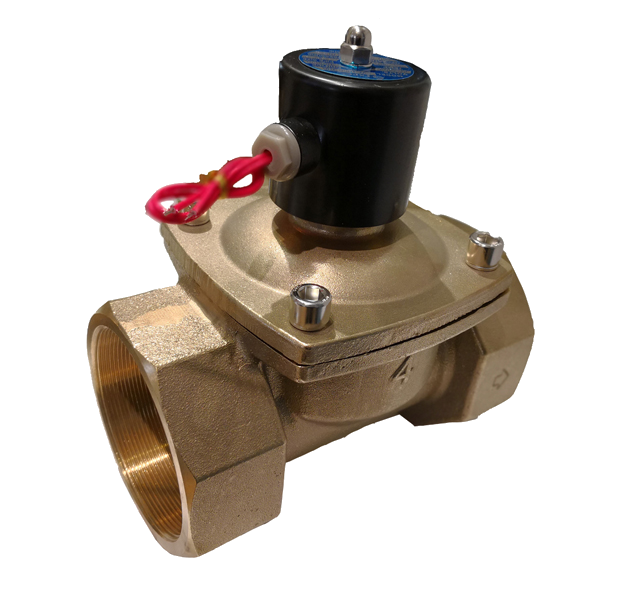
\includegraphics[width=\mythirdmaxsizeimageinsidetable]{chapter5/tablas comparativas/electrovalvula 1.png} \\ 
			%\begin{myflushcenter}
			%	{\footnotesize Nombre imagen}
			%\end{myflushcenter}
		\end{minipage} 
		&
		\begin{minipage}{\mythirdmaxsizeofcontenttable}
			\centering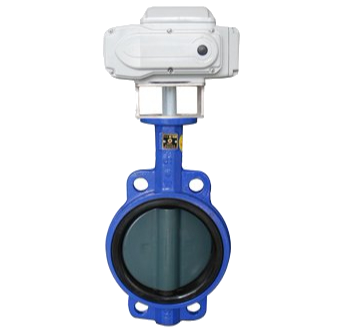
\includegraphics[width=\mythirdmaxsizeimageinsidetable]{chapter5/tablas comparativas/electrovalvula 2.png} \\ 
			%\begin{myflushcenter}
			%	{\footnotesize Nombre imagen}
			%\end{myflushcenter}
		\end{minipage} 
		&
		\begin{minipage}{\mythirdmaxsizeofcontenttable}
			\centering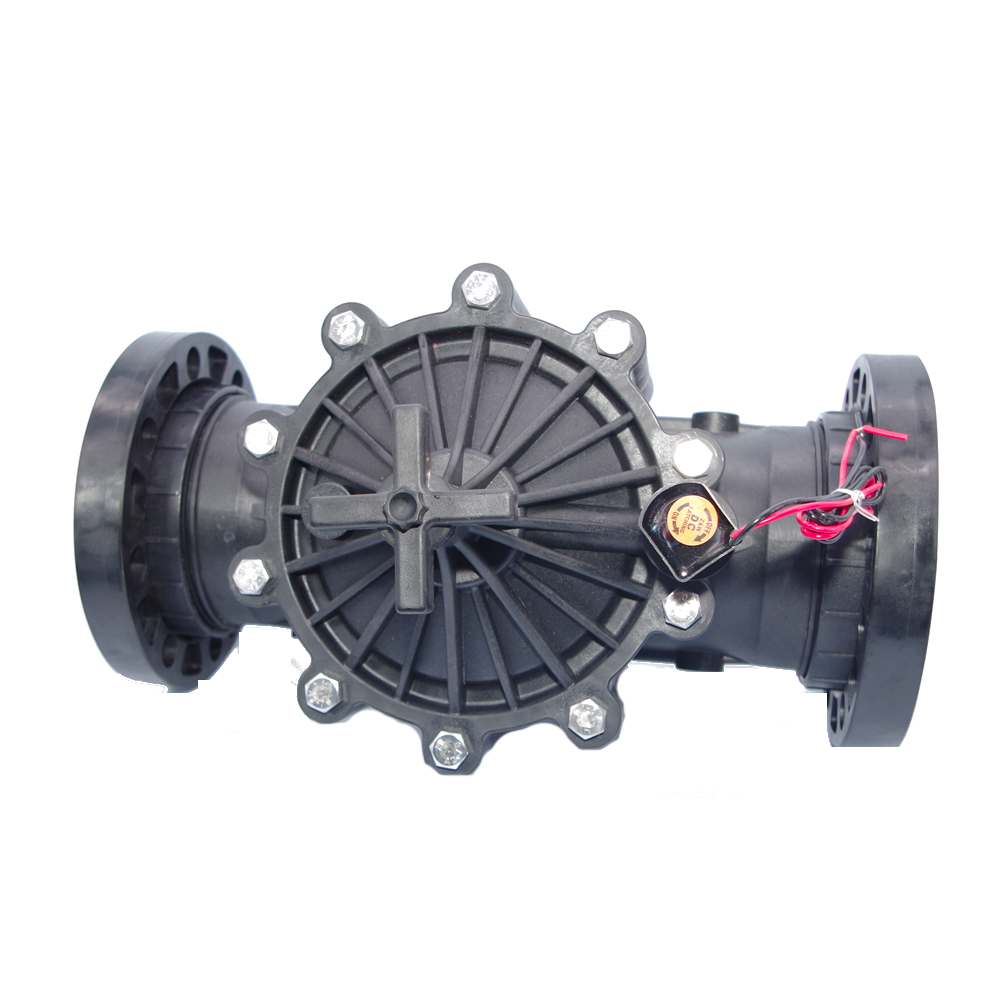
\includegraphics[width=\mythirdmaxsizeimageinsidetable]{chapter5/tablas comparativas/electrovalvula 3.png} \\ 
			%\begin{myflushcenter}
			%	{\footnotesize Nombre imagen}
			%\end{myflushcenter}
		\end{minipage}	\\ \hline
		\multicolumn{1}{|l|}{\textbf{Fabricante}} & - & Xhnotion & TF & AFK \\ \hline
		\multicolumn{1}{|l|}{\textbf{Voltaje de alimentación ($V$)}} & 24 & 24 & 12/24/48 & 24 \\ \hline
		\multicolumn{1}{|l|}{\textbf{Diámetro interno ($in.$)}} & - & Hasta 4 & Hasta 7 & Hasta 4 \\ \hline
		\multicolumn{1}{|l|}{\textbf{Líquidos}} & Agua & Aire/Agua/Aceite & Gas/Agua & Agua \\ \hline
		\multicolumn{1}{|l|}{\textbf{Material}} & - & Latón & Plás./Ac. Inox./Hierro & Plás. + NBR\\ \hline
		\multicolumn{1}{|l|}{\textbf{Tipo de conexión}} & - & Hembra & Hembra & Macho/Hembra \\ \hline
		\multicolumn{1}{|l|}{\textbf{Presión máxima operativa ($kPa$)}} & 550 & - & 4000 & 1400 \\ \hline
		\multicolumn{1}{|l|}{\textbf{Tipo}} & - & Solenoide & Mariposa & Solenoide \\ \hline
		\multicolumn{1}{|l|}{\textbf{Certificados}} & - & ISO 9001:2008 & - & - \\ \hline
		\multicolumn{1}{|l|}{\textbf{Consumo de potencia ($W$)}} & - & - & 100 & - \\ \hline
		\multicolumn{1}{|l|}{\textbf{Temperatura operativa (°$C$)}} & [-10; 40] & [-25; 60] & [-25; 60] & [-20 ; 43] \\ \hline
		\multicolumn{1}{|l|}{\textbf{Peso aproximado ($kg$)}} & - & - & 12 & - \\ \hline
		\multicolumn{1}{|l|}{\textbf{Precio ($S/$)}} & - & 244.12 & 287.20 & 642.61 \\ \hline		
	\end{tabular}	
	\begin{myflushcenteraftertable}			
		Fuente: Imágenes de dominio público y elaboración propia. Hoja de datos técnica (\textit{Datasheet}) en el Anexo. \\
		Tasa de cambio de USD a PEN: S/ 3.59.
	\end{myflushcenteraftertable}
\end{mytable}

Se escoge la válvula del fabricante TF modelo CTB100 debido a que cuenta con un control más complejo al modelo 2W, que si bien su diseño es más simple el control se desplaza al microprocesador. Además, esta electroválvula cumple con el objetivo de regular la apertura de la compuerta que impide el paso de caudal de agua.

%% NUEVO SECCION X.X.X.
\subsection{Selección de sensores de presión}

Los sensores de presión se usan para medir el caudal de forma indirecta y poder controlar la electroválvula. En la sección de control se explica a detalle este proceso. En la Tabla \ref{tab:tabla comparativa de sensores de presion} se presenta una comparación técnica de los sensores de presión.

\begin{mytable}[H]
 	\footnotesize\centering
 	\caption{Tabla comparativa de sensores de presión}
 	\label{tab:tabla comparativa de sensores de presion}
 	\begin{tabular}{l|c|c|c|c|}
 		\cline{2-5}
 		\multicolumn{1}{c|}{\textbf{}} & \textbf{\begin{tabular}[c]{@{}c@{}}Requisitos\\ mínimos\end{tabular}} & \textbf{FST800-211A} & \textbf{WNK80MA} & \textbf{T2000-191202} \\ \hline
 		\multicolumn{1}{|l|}{\textbf{Figura}}   & -   
 		&
 		\begin{minipage}{\mythirdmaxsizeofcontenttable}
 			\centering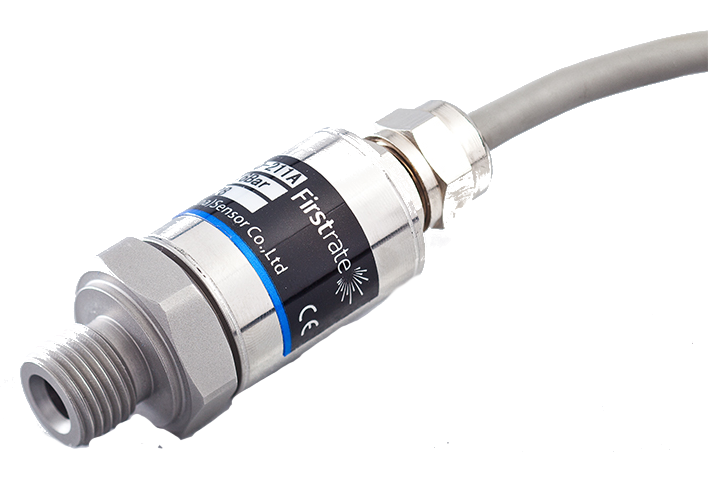
\includegraphics[width=\mythirdmaxsizeimageinsidetable]{chapter5/tablas comparativas/sensor de presion 1.png} \\ 
 			%\begin{myflushcenter}
 			%	{\footnotesize Nombre imagen}
 			%\end{myflushcenter}
 		\end{minipage} 
 		&
 		\begin{minipage}{\mythirdmaxsizeofcontenttable}
 			\centering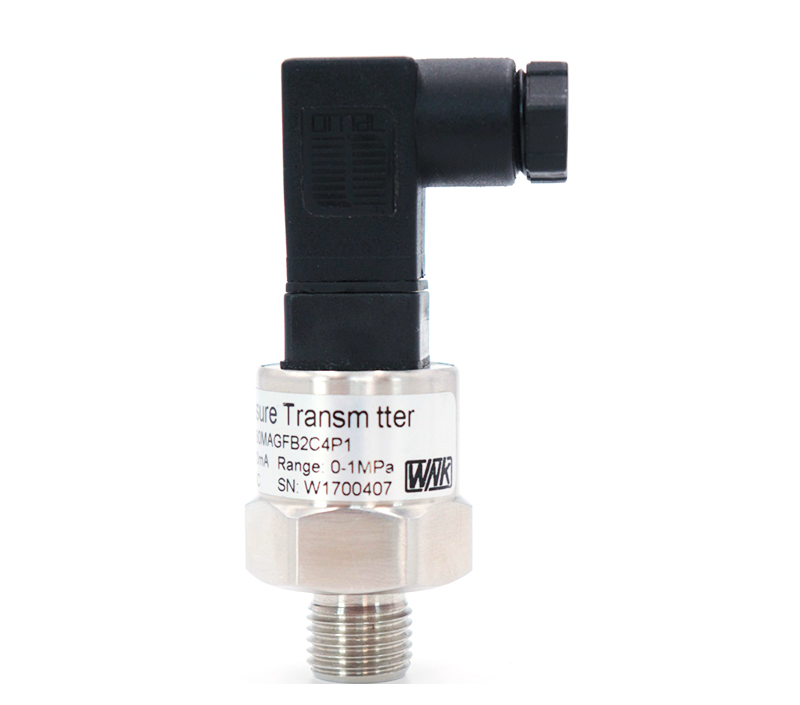
\includegraphics[width=\mythirdmaxsizeimageinsidetable]{chapter5/tablas comparativas/sensor de presion 2.png} \\ 
 			%\begin{myflushcenter}
 			%	{\footnotesize Nombre imagen}
 			%\end{myflushcenter}
 		\end{minipage} 
 		&
 		\begin{minipage}{\mythirdmaxsizeofcontenttable}
 			\centering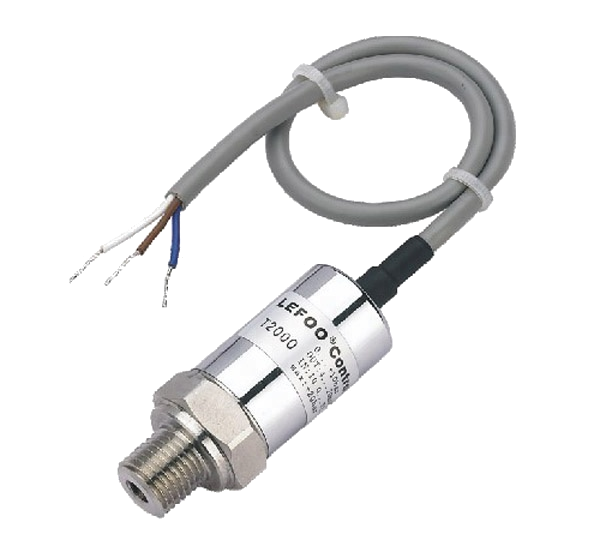
\includegraphics[width=\mythirdmaxsizeimageinsidetable]{chapter5/tablas comparativas/sensor de presion 3.png} \\ 
 			%\begin{myflushcenter}
 			%	{\footnotesize Nombre imagen}
 			%\end{myflushcenter}
 		\end{minipage}	\\ \hline	
 		\multicolumn{1}{|l|}{\textbf{Fabricante}} & - & FirstRate & WNK & LEFOO \\ \hline
 		\multicolumn{1}{|l|}{\textbf{Voltaje de alimentación ($V$)}} & 12 & [9; 30] & 3.3/5/12/24 & [10; 30] \\ \hline
 		\multicolumn{1}{|l|}{\textbf{Voltaje de salida ($V$)}} & - & [0.5; 4.5] & [1; 5] & [0; 10] \\ \hline
 		\multicolumn{1}{|l|}{\textbf{Corriente de salida ($mA$)}} & - & [4; 20] & [4; 20] & [4; 20] \\ \hline
 		\multicolumn{1}{|l|}{\textbf{Temperatura operativa (°$C$)}} & [-10; 40] & [-40; 85] & [-20; 85] & [-10 ; 80] \\ \hline
 		\multicolumn{1}{|l|}{\textbf{Protección ($IP$)}} & - & $IP65$ & $IP65$ & $IP65$ \\ \hline
 		\multicolumn{1}{|l|}{\textbf{Certificados}} & - & CE RoHS & CE RoHS \& ISO & ECM \\ \hline
 		\multicolumn{1}{|l|}{\textbf{Precisión ($Pa$)}} & - & - & 5000 & - \\ \hline
 		\multicolumn{1}{|l|}{\textbf{Presión máxima ($kPa$)}} & 550 & [100; 60000] & [20; 25000] & [20; 25000] \\ \hline
 		\multicolumn{1}{|l|}{\textbf{Peso aproximado ($kg$)}} & - & 0.1 & 0.1 & - \\ \hline
 		\multicolumn{1}{|l|}{\textbf{Precio ($S/$)}} & - & 78.98 & 43.08 & 89.75 \\ \hline		
 	\end{tabular}	
 	\begin{myflushcenteraftertable}			
 		Fuente: Imágenes de dominio público y elaboración propia. Hoja de datos técnica (\textit{Datasheet}) en el Anexo. \\
 		Tasa de cambio de USD a PEN: S/ 3.59.
 	\end{myflushcenteraftertable}
\end{mytable}

El sensor de presión WNK80MA de la empresa manufacturera WNK es escogido porque representa los requisitos mínimos a un menor precio, sin escatimar en características como nivel de protección, certificados y máxima presión que soporta el componente.	

%----------------------------------------------------------------------------------------
%	Capítulo 5 
%----------------------------------------------------------------------------------------
\pagestyle{myportland}
%\pagenumbering{arabic}
\doublespacing
\chapter[\quad\quad\quad\quad ----- Diseño de subsistema de procesamiento de imágenes]{\\ Diseño de subsistema de procesamiento de imágenes}
\thispagestyle{myportland}

Este subsistema consiste obtener una serie de imágenes de una trucha en tránsito e indicar al sistema a dónde debería dirigirse una trucha determinada. El subsistema debe clasificar y contar truchas, con dicha finalidad necesita de la selección de una cámara y generar el ambiente adecuado para obtener las imágenes. Explicado los objetivos del subsistema, en las siguientes líneas se detalla: la selección del sensor infrarrojo, la selección de cámara estéreo, la selección de iluminación adecuada y la selección de algoritmos. En la Figura \ref{fig:subsistema de procesamiento de imagenes} se enumera los principales componentes: 1. sensor de presión; 2. reductor de tubería; 3. sensor infrarrojo; 4. adaptador y sensor infrarrojo; 5. cámara estéreo a cierta distancia perpendicular; 6. juego de espejos; 7. tubo transparente.

\begin{myfigure}[H]
	\footnotesize\centering
	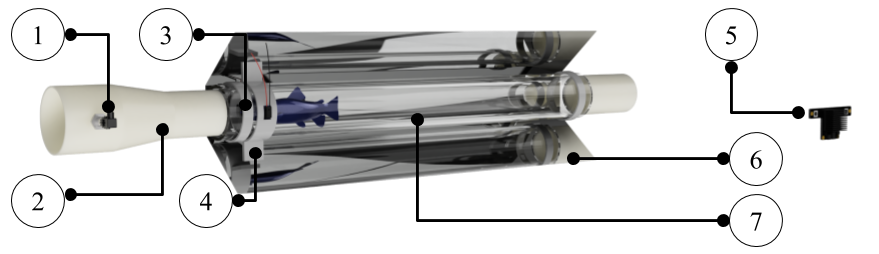
\includegraphics[width=1\textwidth]{chapter5/subensambles/procesamiento de imagenes final.png}
	\caption{Subsistema de procesamiento de imágenes}
	\begin{myflushcenter}
		Fuente: Elaboración propia.
	\end{myflushcenter}
	\label{fig:subsistema de procesamiento de imagenes}
\end{myfigure}
 
%% NUEVO SECCION X.X.
\section{Selección del sensor infrarrojo}

El sensor infrarrojo tiene como objetivo activar el algoritmo de detección y conteo de truchas por un determinado periodo de tiempo con la finalidad de evitar un sobre uso de los recursos computacionales. El sensor infrarrojo está unos centímetros antes de la parte que la cámara captura y su posición es como se muestra en el globo número 4 con su adaptador para la tubería en la Figura \ref{fig:subsistema de procesamiento de imagenes}.

%\begin{myfigure}[H]
%	\footnotesize\centering
%	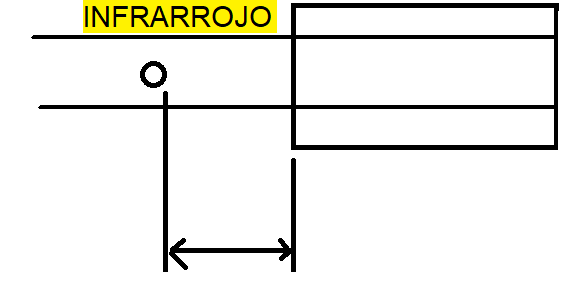
\includegraphics[width=1\textwidth]{chapter5/posicion sensor infrarrojo.png}
%	\caption{Posicionamiento del sensor infrarrojo}
%	\begin{myflushcenter}
%		Fuente: Elaboración propia.
%	\end{myflushcenter}
%	\label{fig:posicion sensor infrarrojo}
%\end{myfigure}

Ya que los haces de luz cambian de dirección debido a la refracción\footnote{\cite{Hecht2017}.}, cuando varía de un medio a otro, se calcula esta desviación para la adecuada detección de objetos que pasen por la tubería. La representación gráfica de la situación se expone en la Figura \ref{fig:analisis de posicion de luz infrarroja}.

\begin{myfigure}[H]
	\footnotesize\centering
	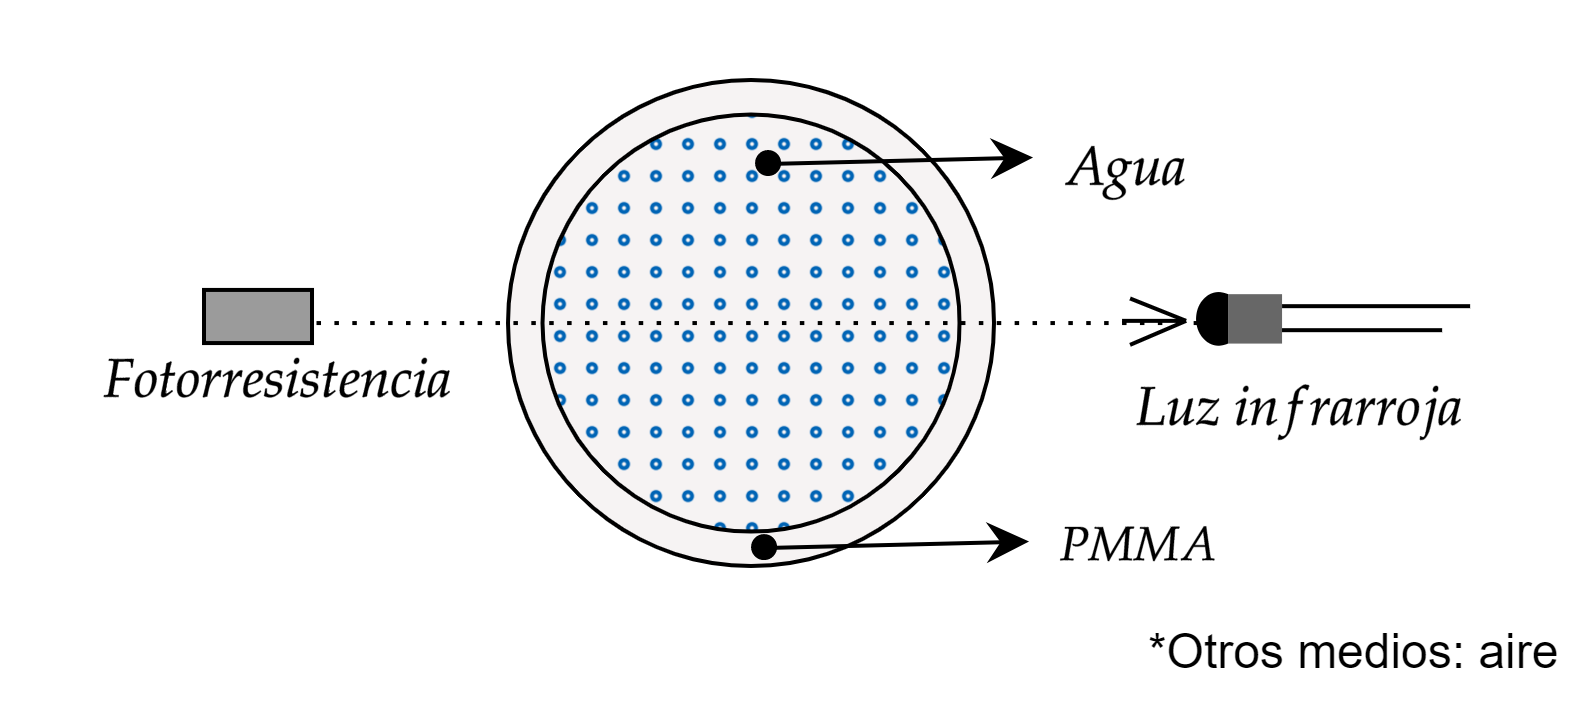
\includegraphics[width=0.75\textwidth]{chapter5/analisis de posicion de luz infrarroja.png}
	\caption{Análisis de posición de luz infrarroja}
	\begin{myflushcenter}
		Fuente: Elaboración propia.
	\end{myflushcenter}
	\label{fig:analisis de posicion de luz infrarroja}
\end{myfigure}

El problema se muestra en la Figura \ref{fig:calculo de posicion de luz infrarroja}. Cabe mencionar que se conocen los siguientes valores $n_{PMMA}=1.5$\footnote{Propiedades ópticas mostradas en la Tabla \ref{tab:tabla comparativa de propiedades entre pmma vs pvdf vs petg}. \cite{Berins1991}}, $n_{aire}\approx1$, $n_{agua}=1.33$\footnote{Índices de refracción: \cite{Hecht2017}.}, $d_{1}=d_{2}=10 mm.$, $e=3 mm.$ y $d_{int}=85 mm.$ ,y se asume, para simplificar el problema, la emisión de la luz como proveniente de un punto único ($S$).

\begin{myfigure}[H]
	\footnotesize\centering
	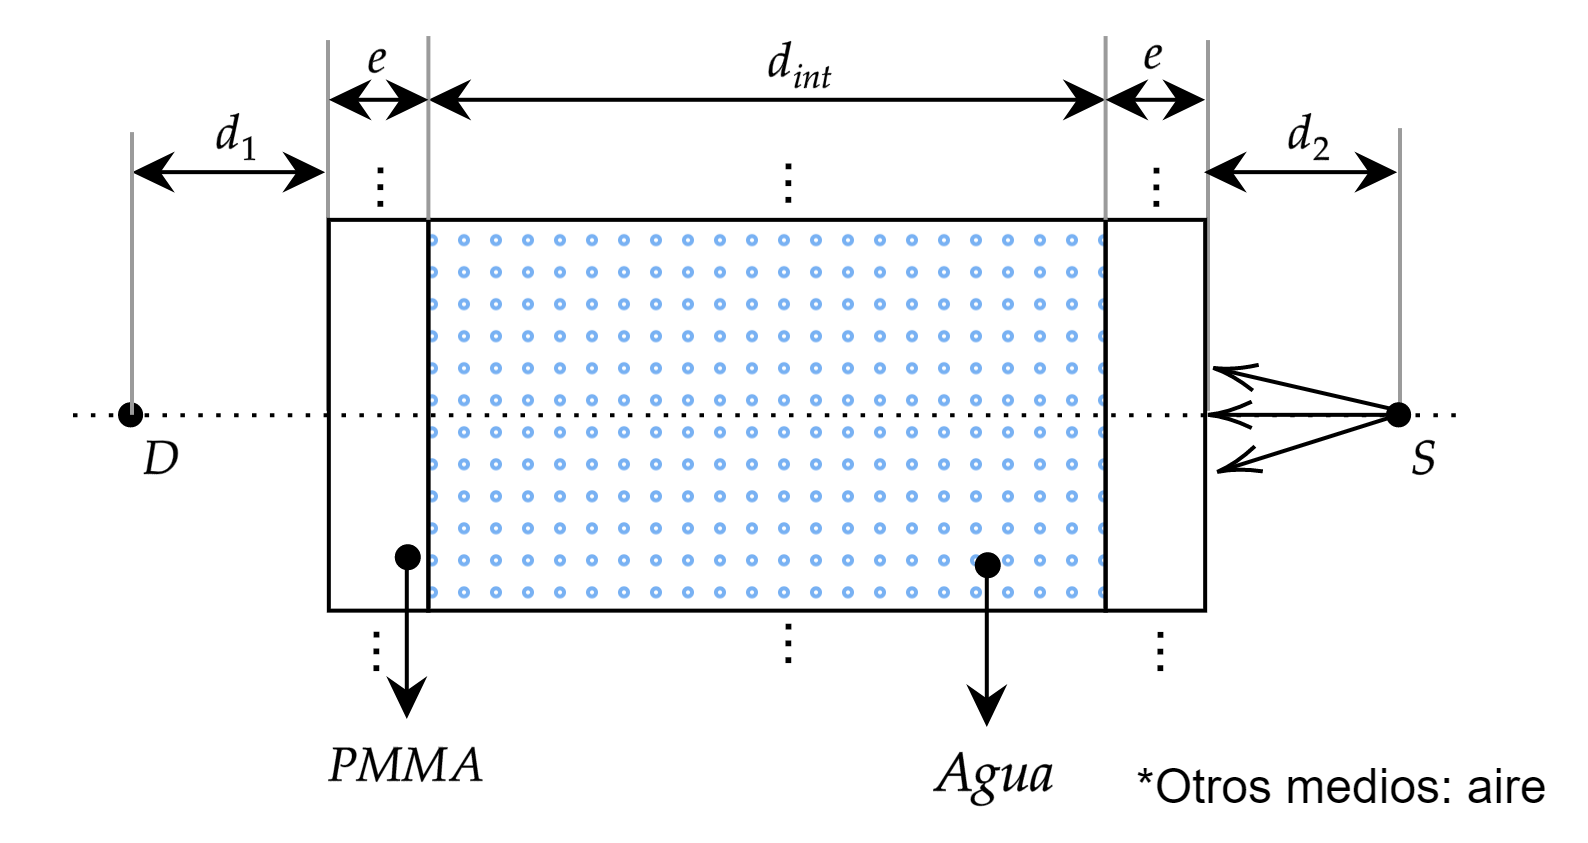
\includegraphics[width=0.75\textwidth]{chapter5/calculo de posicion de luz infrarroja.png}
	\caption{Cálculo de posición de luz infrarroja}
	\begin{myflushcenter}
		Fuente: Elaboración propia.
	\end{myflushcenter}
	\label{fig:calculo de posicion de luz infrarroja}
\end{myfigure}

Para el cálculo de desviación de los haces de luz se emplea la ley de refracción, matemáticamente mostrada en la Ecuación \ref{eq:ecuacion de snell}. Donde: $\theta_{i}$ es el ángulo de incidencia respecto a la normal del primer medio, $\theta_{t}$ es el ángulo de refracción respecto a la normal.

\begin{myequation}\label{eq:ecuacion de snell}
	\begin{split}
		n_{i}*sin(\theta_{i})&=n_{t}*sin(\theta_{t})
	\end{split}		
\end{myequation}

En la Figura \ref{fig:calculo distancia maxima de desviacion de haz de luz en condiciones ideales} se analiza el caso crítico cuando $\theta_{1}\approx5^\circ$. Con la Ecuación \ref{eq:ecuacion de snell} se puede calcular las distancias de desviación por refracción. Por ejemplo, En la Ecuación \ref{eq:calculo distancia maxima de desviacion de haz de luz en condiciones ideales} el valor de $h_{x}$ es la distancia proyectada: $h_{x}=d_{x}*tan(\theta_{x})$.

\begin{myfigure}[H]
	\footnotesize\centering
	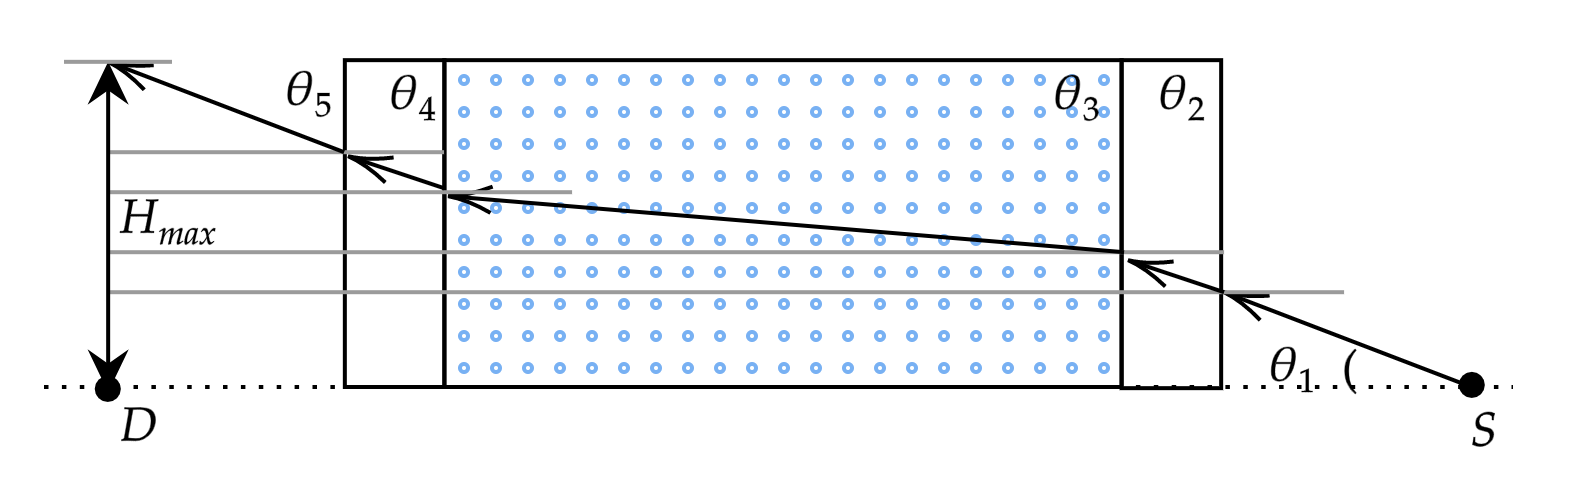
\includegraphics[width=0.75\textwidth]{chapter5/calculo distancia maxima de desviacion de haz de luz en condiciones ideales.png}
	\caption{Cálculo de distancia máxima de desviación de haz de luz en condiciones ideales.}
	\begin{myflushcenter}
		Fuente: Elaboración propia.
	\end{myflushcenter}
	\label{fig:calculo distancia maxima de desviacion de haz de luz en condiciones ideales}
\end{myfigure}

\begin{myequation}\label{eq:calculo distancia maxima de desviacion de haz de luz en condiciones ideales}
	\begin{split}
		H_{max}&=h_{1}+h_{2}+h_{3}+h_{4}+h_{5} \\
		H_{max}&=10*tan(\theta_{1})+3*tan(\theta_{2})+85*tan(\theta_{3})+3*tan(\theta_{4})+10*tan(\theta_{5}) \\
		H_{max}&=10*tan(5^\circ)+3*tan(3.33^\circ)+85*tan(3.76^\circ)+3*tan(3.33^\circ)+10*tan(5^\circ) \\
		H_{max}&=7.685 mm.
	\end{split}		
\end{myequation}

Para una óptima recepción se propone llegar como mínimo 75\% de haces de luz. Esto quiere decir que del diámetro ideal del dispositivo receptor debe ser de 15.4 mm y el óptimo 13.33 mm.\footnote{$d_{ideal-receptor}=2*H_{max}=15.4 mm.$ y $d_{75\%-receptor}=\sqrt{0.75*15.4^2}=13.33 mm.$ } Finalmente, los requerimientos mínimos que debe tener el sensor infrarrojo óptimo y comparaciones técnicas de los dispositivos comerciales que cumplen con los requerimientos se muestran en la Tabla \ref{tab:tabla comparativa de sensores infrarrojos}.

\begin{mytable}[H]
	\footnotesize\centering
	\caption{Tabla comparativa de sensores infrarrojos.}
	\label{tab:tabla comparativa de sensores infrarrojos}
	\begin{tabular}{l|c|c|c|c|}
		\cline{2-5}
		\multicolumn{1}{c|}{\textbf{}}            & \textbf{\begin{tabular}[c]{@{}c@{}}Requisitos\\ mínimos\end{tabular}} &
		\multicolumn{1}{|l|}{
			\begin{minipage}{\mythirdmaxsizeofcontenttable}	
				\begin{myflushcenterinsidetable}
					\textbf{HD-DS25 CM-3MM}
				\end{myflushcenterinsidetable}				
			\end{minipage}
		}&
		\multicolumn{1}{|l|}{		
			\begin{minipage}{\mythirdmaxsizeofcontenttable}	
				\begin{myflushcenterinsidetable}
					\textbf{QT50CM}
				\end{myflushcenterinsidetable}				
			\end{minipage}	
		}&
		\multicolumn{1}{|l|}{			
			\begin{minipage}{\mythirdmaxsizeofcontenttable}	
				\begin{myflushcenterinsidetable}
					\textbf{GP2Y0A 21YK0F}
				\end{myflushcenterinsidetable}				
			\end{minipage}
		}  \\ \hline
		\multicolumn{1}{|l|}{\textbf{Figura}} & - 
		&		  
		\begin{minipage}{\mythirdmaxsizeofcontenttable}
			\centering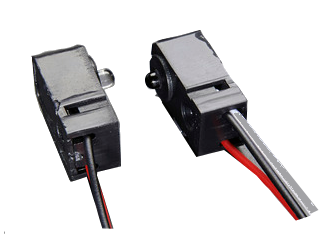
\includegraphics[width=\mythirdmaxsizeimageinsidetable]{chapter5/tablas comparativas/sensor infrarrojo 1.png} \\ 
			%\begin{myflushcenter}
			%	{\footnotesize Nombre imagen}
			%\end{myflushcenter}
		\end{minipage}
		&		  
		\begin{minipage}{\mythirdmaxsizeofcontenttable}
			\centering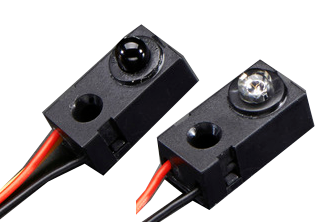
\includegraphics[width=\mythirdmaxsizeimageinsidetable]{chapter5/tablas comparativas/sensor infrarrojo 2.png} \\ 
			%\begin{myflushcenter}
			%	{\footnotesize Nombre imagen}
			%\end{myflushcenter}
		\end{minipage}
		&  
		\begin{minipage}{\mythirdmaxsizeofcontenttable}
			\centering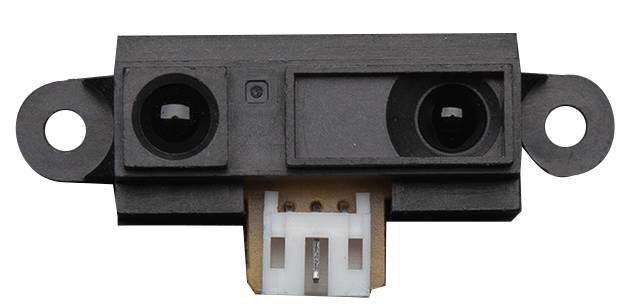
\includegraphics[width=\mythirdmaxsizeimageinsidetable]{chapter5/tablas comparativas/sensor infrarrojo 3.png} \\ 
			%\begin{myflushcenter}
			%	{\footnotesize Nombre imagen}
			%\end{myflushcenter}
		\end{minipage}\\ \hline
		\multicolumn{1}{|l|}{\textbf{Fabricante}} 
		& - & Adafruit & Adafruit & SHARP\\ \hline
		\multicolumn{1}{|l|}{
			\begin{minipage}{\myforthmaxsizeofcontenttable}	
				\textbf{Tipo de comunicación}
			\end{minipage}
		} & - & [0;VCC] & [0;VCC] & Analógico         \\ \hline
		\multicolumn{1}{|l|}{
			\begin{minipage}{\myforthmaxsizeofcontenttable}	
				\textbf{Área mínima circular de receptor ($mm^2$)}
			\end{minipage}
		} & 15.4 & 28.27 & 78.54 & 162.86         \\ \hline
		\multicolumn{1}{|l|}{
			\begin{minipage}{\myforthmaxsizeofcontenttable}	
				\textbf{Ángulo de visión/recepción (°)}
			\end{minipage}
		} & 5 & 10 & 10 & -         \\ \hline
		\multicolumn{1}{|l|}{
			\begin{minipage}{\myforthmaxsizeofcontenttable}	
				\textbf{Distancia de detección ($mm.$)}
			\end{minipage}
		} & 170 & [0;250] & [0;500] & [100;800] \\ \hline
		\multicolumn{1}{|l|}{
			\begin{minipage}{\myforthmaxsizeofcontenttable}	
				\textbf{Longitud de onda infrarroja recomendada ($nm$)}
			\end{minipage}
		} & 850 & - & - & 870$\pm$70 \\ \hline
		\multicolumn{1}{|l|}{
			\begin{minipage}{\myforthmaxsizeofcontenttable}	
				\textbf{Voltaje operativo VCC ($V$)}
			\end{minipage}
		} & 5  & [3.0;5.5] & [3.0;5.5] & [4.5;5.5]         \\ \hline
		\multicolumn{1}{|l|}{
			\begin{minipage}{\myforthmaxsizeofcontenttable}	
				\textbf{Consumo de corriente ($mA$)}
			\end{minipage}
		} & -  & 100 & 100 & 30         \\ \hline
		\multicolumn{1}{|l|}{
			\begin{minipage}{\myforthmaxsizeofcontenttable}	
				\textbf{Temperatura operativa (°$C$)}
			\end{minipage}
		} & [-10;40] & [-25;60] & [-25;60] & [-10;60] \\ \hline
		\multicolumn{1}{|l|}{
			\begin{minipage}{\myforthmaxsizeofcontenttable}	
				\textbf{Precio ($S/$)}
			\end{minipage}
		} & - & 7.00 & 23.32 & 53.68 \\ \hline
	\end{tabular}
	\begin{myflushcenteraftertable}	
		Fuente: Marktech Optoelectronics y elaboración propia. Hoja de datos técnica (\textit{Datasheet}) en el Anexo.\\
		Tasa de cambio de USD a PEN: S/ 3.59.
	\end{myflushcenteraftertable}
\end{mytable}

De la Tabla \ref{tab:tabla comparativa de sensores infrarrojos} se visualiza que las principales diferencias de las alternativas se basan en el área de los actuadores infrarrojos del emisor y su sensado en el receptor, y la distancia máxima que puede detectar. La distancia máxima a medir en el sistema, es el diámetro de la tubería que no es mayor a $4 \; in. \approx 100 \; mm.$ adicional al mecanismo que los posicionará no debería exceder de los $170 \; mm.$. Entonces, se escoge el modelo HD-DS25CM-3MM que cumple con estas características al menor precio.

%% NUEVO SECCION X.X.
\section{Selección de cámaras} 

En el sistema se emplea dos cámaras con distintos requerimientos técnicos. Por un lado, una cámara estéreo se encarga de capturar imágenes que van a ser procesadas por algoritmos de detección y conteo de truchas. Por otro lado, una cámara normal registra la trayectoria de las truchas que en la distribución de estas a los canales de salida definidos por los algoritmos. 


%% NUEVO SECCION X.X.X.
\subsection{Cálculo de distancias apropiadas de las cámaras}

El área que se debe captar sobre el proceso, sin las tuberías transparentes, se representan  en una vista frontal y de perfil en la Figura \ref{fig:distancia entre juego de espejos y camara estereo}. Donde: $d$ es la distancia entre el juego de espejos y la cámara, $\alpha$ es el HDFV\footnote{Campo de visión horizontal.}, $\beta$ es el VDFV\footnote{Campo de visión vertical.}, $A$ es la altura del área proyectada y $L$ es la largo del área proyectada del juego de espejos.

\begin{myfigure}[H]
	\footnotesize\centering
	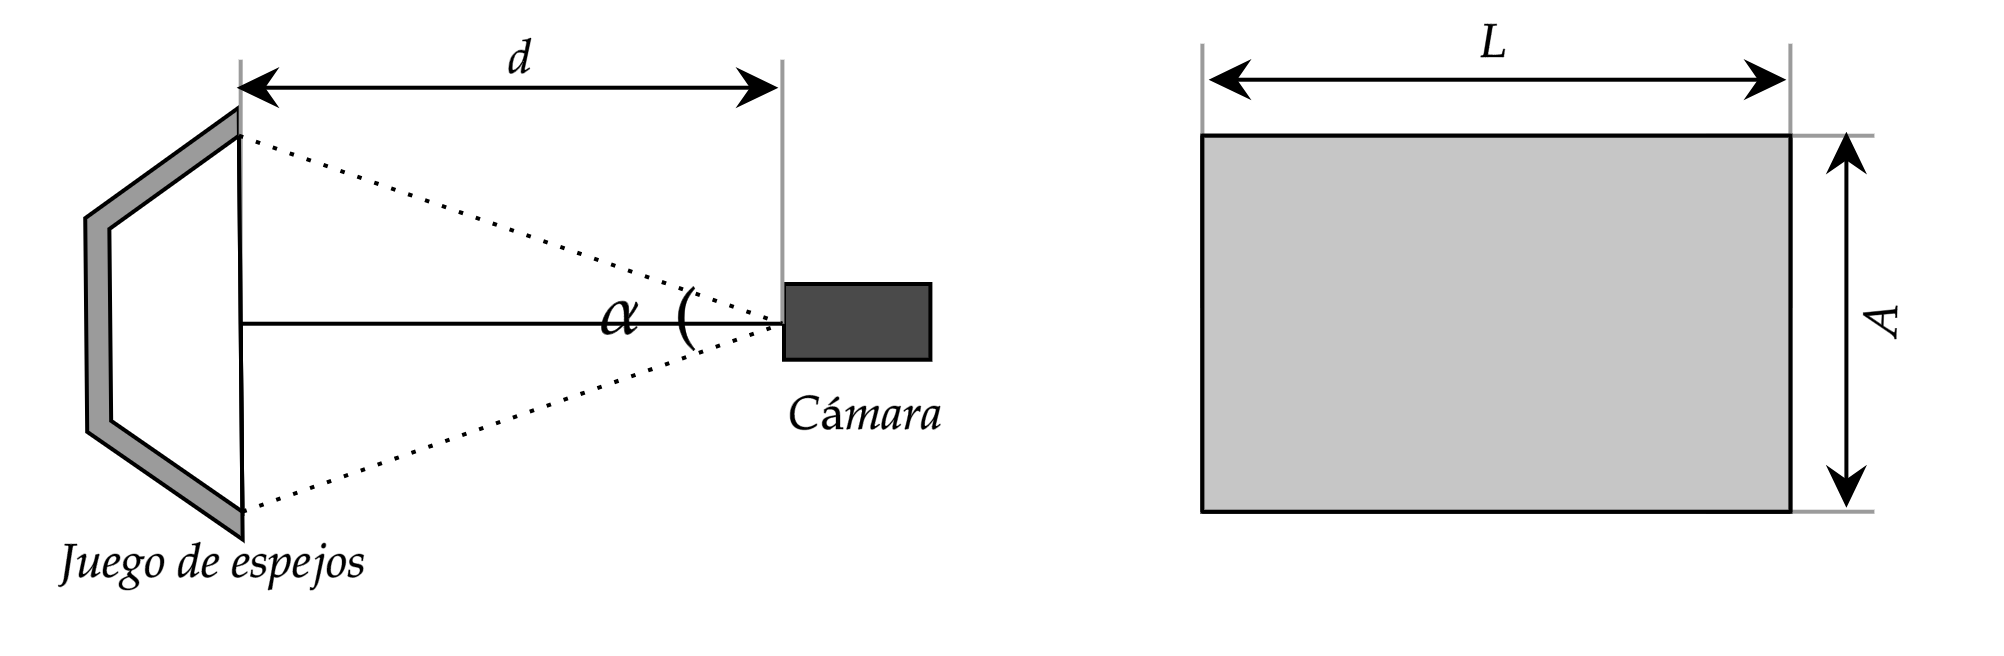
\includegraphics[width=1\textwidth]{chapter5/distancia entre juego de espejos y camara estereo.png}
	\caption{Distancia entre juego de espejos y cámara estéreo}
	\begin{myflushcenter}
		Fuente: Elaboración propia.
	\end{myflushcenter}
	\label{fig:distancia entre juego de espejos y camara estereo}
\end{myfigure}

De la geometría se obtiene los valores de $\alpha$ y $\beta$, que dependen de las otras variables. El posicionamiento de la cámara ($d$) estéreo estará sujeto a sus valores de HDFV y VDFV como se muestra en la Ecuación \ref{eq:calculo beta de distancia entre espejos y camara estereo} y \ref{eq:calculo alfa de distancia entre espejos y camara estereo}, respectivamente.
	
\begin{myfigure}[H]
	\footnotesize\centering
	\includegraphics[width=1\textwidth]{chapter5/calculo de distancia entre espejos y camara estereo.png}
	\caption{Cálculo de distancia apropiada para la cámara estéreo}
	\begin{myflushcenter}
		Fuente: Elaboración propia.
	\end{myflushcenter}
	\label{fig:calculo de distancia entre espejos y camara estereo}
\end{myfigure}

\begin{myequation}\label{eq:calculo alfa de distancia entre espejos y camara estereo}
	\begin{split}
		tan(\alpha_{min}/2)&=\frac{A/2}{d}\\
		\alpha_{min}&=2*atan(\frac{A}{2*d})\\
	\end{split}		
\end{myequation}

\begin{myequation}\label{eq:calculo beta de distancia entre espejos y camara estereo}
	\begin{split}
		tan(\beta_{min}/2)&=\frac{L/2}{d}\\
		\beta_{min}&=2*atan(\frac{L}{2*d})\\
	\end{split}		
\end{myequation}

%% NUEVO SECCION X.X.X.
\subsection{Cálculo de cuadros por segundo (fps) necesarios para la cámara estéreo}

Con el objetivo de calcular los cuadros por segundo necesarios, se muestra en la Figura \ref{fig:grafica tamano y velocidad de nado trucha arcoiris} una aproximación lineal entre el peso ($g$) y la velocidad de nado ($cm/s$) de una trucha de la especie en cuestión. Dicho nado es contracorriente y de forma aleatoria, en el presente estudio se utiliza dicha información para simplificar el análisis\footnote{Es necesario elaborar un estudio detallado de la velocidad de nado dentro de sistemas acorde al propuesto. El estudio  \cite{Borisovich2016} asegura que se pudo capturar imágenes a 25 Hz de una tubería de 180 $mm.$ de diámetro a una velocidad de 5-8 $m/s$}.

\begin{myfigure}[H]
	\footnotesize\centering
	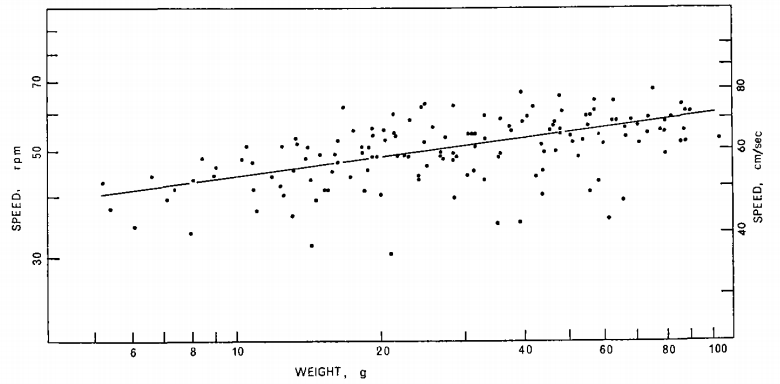
\includegraphics[width=1\textwidth]{chapter5/grafica tamano y velocidad de nado trucha arcoiris.png}
	\caption{Aproximación lineal de la relación entre peso y la velocidad de nado de truchas arcoíris}
	\begin{myflushcenter}
		Fuente: \cite{Fry1970}
	\end{myflushcenter}
	\label{fig:grafica tamano y velocidad de nado trucha arcoiris}
\end{myfigure}	

En la Ecuación \ref{eq:ecuacion relacion tamano y velocidad de nado de trucha arcoiris} se muestra la relación (regresión lineal) entre \textit{X: peso de la trucha ($g$)} e \textit{Y: velocidad de nado ($cm/s$)} con un error \textit{Z= $0.033$}. 

\begin{myequation} \label{eq:ecuacion relacion tamano y velocidad de nado de trucha arcoiris}
	Y\approx0.2828*X+48
\end{myequation}

En el caso de este trabajo, la dimensión máxima y mínima de las truchas arcoíris son de 20 cm y 15 cm, respectivamente. De la Tabla \textit{Clasificación de truchas por etapas de producción}\footnote{\cite{DiazVergara2020}} podemos obtener los gramos mediante interpolación lineal para cada límite: valores mínimo-máximo son 153 y 199 \textit{$g$}, respectivamente. Utilizando los valores antes indicados y empleando la Ecuación \ref{eq:ecuacion relacion tamano y velocidad de nado de trucha arcoiris} obtenemos los límites dentro del rango $[91.26; 104.268] (cm/s)$. Luego de escoger la máxima velocidad con redondeo hacia arriba $v_{max}=105cm/s$) se duplica esta para que la trucha con nado a contracorriente sea desplazada a la velocidad máxima en dirección opuesta. Además, se analiza la cantidad de cuadros por segundo necesario: el recorrido entre un fotograma y otro debe ser menor o igual a dos centímetros. Se establece una distancia de un metro para la parte de visión y computadora por lo que la división de $1000/20$ da un valor de $fps_{min}=50$. Entonces, se realizarán aproximadamente 50 capturas de fotogramas en un segundo.\footnote{En dicha imagen pueden haber más de una trucha en tránsito.}

%% NUEVO SECCION X.X.X.
\subsection{Selección de cámara estéreo}

El objetivo de la cámara estéreo es la de obtener fotos por determinado periodo de tiempo designado por los algoritmos de procesamiento de imágenes. Con el fin de cumplir el objetivo mencionado deben cumplirse requerimientos técnicos: fotografiar a la trucha con un enfoque aceptable que permita distinguir a la trucha adecuadamente, ángulo de visión horizontal y vertical, resolución, entre otros. En la Figura \ref{fig:diagrama esquematico camara estereo y dependencia de la distancia del objeto} se visualiza un diagrama referencial de una cámara estéreo, con la cuál podemos obtener distancias a partir de dos imágenes. 

\begin{myfigure}[H]
	\footnotesize\centering
	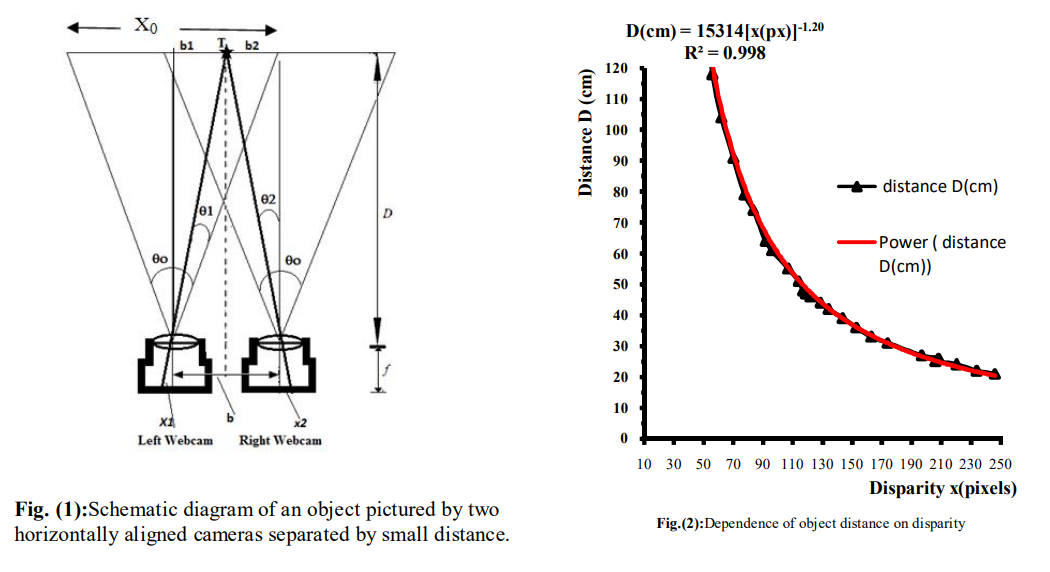
\includegraphics[width=1\textwidth]{chapter5/diagrama esquematico camara estereo y dependencia de la distancia del objeto.png}
	\caption[Diagrama esquemático y dependencia de la distancia del objeto seguido por una cámara estéreo.]{(Izq.) Diagrama esquemático de un objeto representado por dos cámaras alineadas horizontalmente separadas por una pequeña distancia. (Der.) Dependencia de la distancia del objeto en la disparidad.}
	\begin{myflushcenter}
		Fuente: \cite{Mahammed2013}
	\end{myflushcenter}
	\label{fig:diagrama esquematico camara estereo y dependencia de la distancia del objeto}
\end{myfigure}

En el campo de la acuicultura, ante la inexistente literatura sobre este tipo de estudios, se brinda un estudio similar de medición de vehículos autónomos brindado en \cite{Zaarane2020} (Figura \ref{fig:medicion de distancia con distintas distancias}) del que este estudio se guía para la obtención de distancias más cercanas a las reales con el uso de la profundidad gracias al sistema de cámara estéreo .

\begin{myfigure}[H]
	\footnotesize\centering
	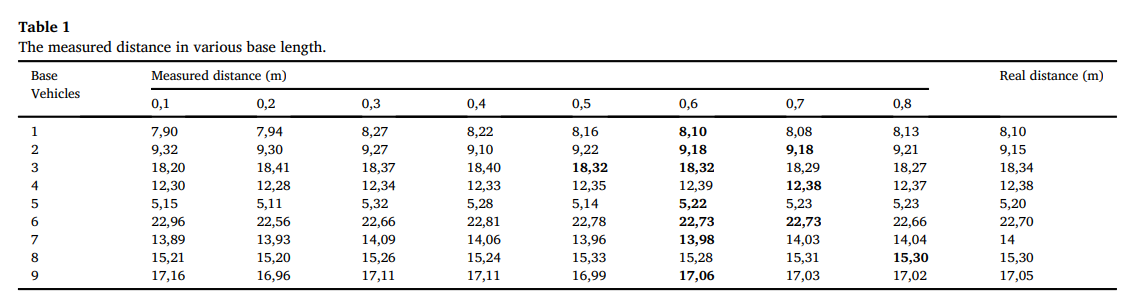
\includegraphics[width=1\textwidth]{chapter5/medicion de distancia con distintas distancias.png}
	\caption{Pruebas de medición con distintas distancias al objeto.}
	\begin{myflushcenter}
		Fuente: \cite{Zaarane2020}
	\end{myflushcenter}
	\label{fig:medicion de distancia con distintas distancias}
\end{myfigure}
	
%- Tamaño de píxeles requerido \\
%- Cantidad de frames (80 fps con 3-4L/s) (Falta calcular con lo que hemos calculado 16 cm/s) \\ 
%- La inclinación hace que el pez no tenga velocidad hacia arriba \\

En la Tabla \ref{tab:tabla comparativa de camaras estereo} se muestra tanto los requerimientos mínimos como las cámaras estéreo candidatas para el sistema. El cálculo mencionado en la sección anterior se calcula luego de escoger una de entre las tres opciones mostradas.

\begin{savenotes}
\begin{mytable}[H]
	\footnotesize\centering
	\caption{Tabla comparativa de cámaras estéreo.}
	\label{tab:tabla comparativa de camaras estereo}
	\begin{tabular}{l|c|c|c|c|}
		\cline{2-5}
		\multicolumn{1}{c|}{\textbf{}}            & \textbf{\begin{tabular}[c]{@{}c@{}}Requisitos\\ mínimos\end{tabular}} & 
		\multicolumn{1}{|l|}{				
			\begin{minipage}{\mythirdmaxsizeofcontenttable}
				\begin{myflushcenterinsidetable}
					\textbf{OAK-D}
				\end{myflushcenterinsidetable}
			\end{minipage}
		}&
		\multicolumn{1}{|l|}{				
			\begin{minipage}{\mythirdmaxsizeofcontenttable}	
				\begin{myflushcenterinsidetable}
					\textbf{B0263}
				\end{myflushcenterinsidetable}
			\end{minipage}
		}&
		\multicolumn{1}{|l|}{				
			\begin{minipage}{\mythirdmaxsizeofcontenttable}	
				\begin{myflushcenterinsidetable}
					\textbf{B0204}
				\end{myflushcenterinsidetable}
			\end{minipage}
		}  \\ \hline
		\multicolumn{1}{|l|}{\textbf{Figura}} & - 
		&		  
		\begin{minipage}{\mythirdmaxsizeofcontenttable}
			\centering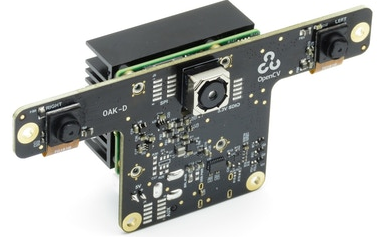
\includegraphics[width=\mythirdmaxsizeimageinsidetable]{chapter5/tablas comparativas/camara estereo 1.png} \\ 
			%\begin{myflushcenter}
			%	{\footnotesize Nombre imagen}
			%\end{myflushcenter}
		\end{minipage}
		&		  
		\begin{minipage}{\mythirdmaxsizeofcontenttable}
			\centering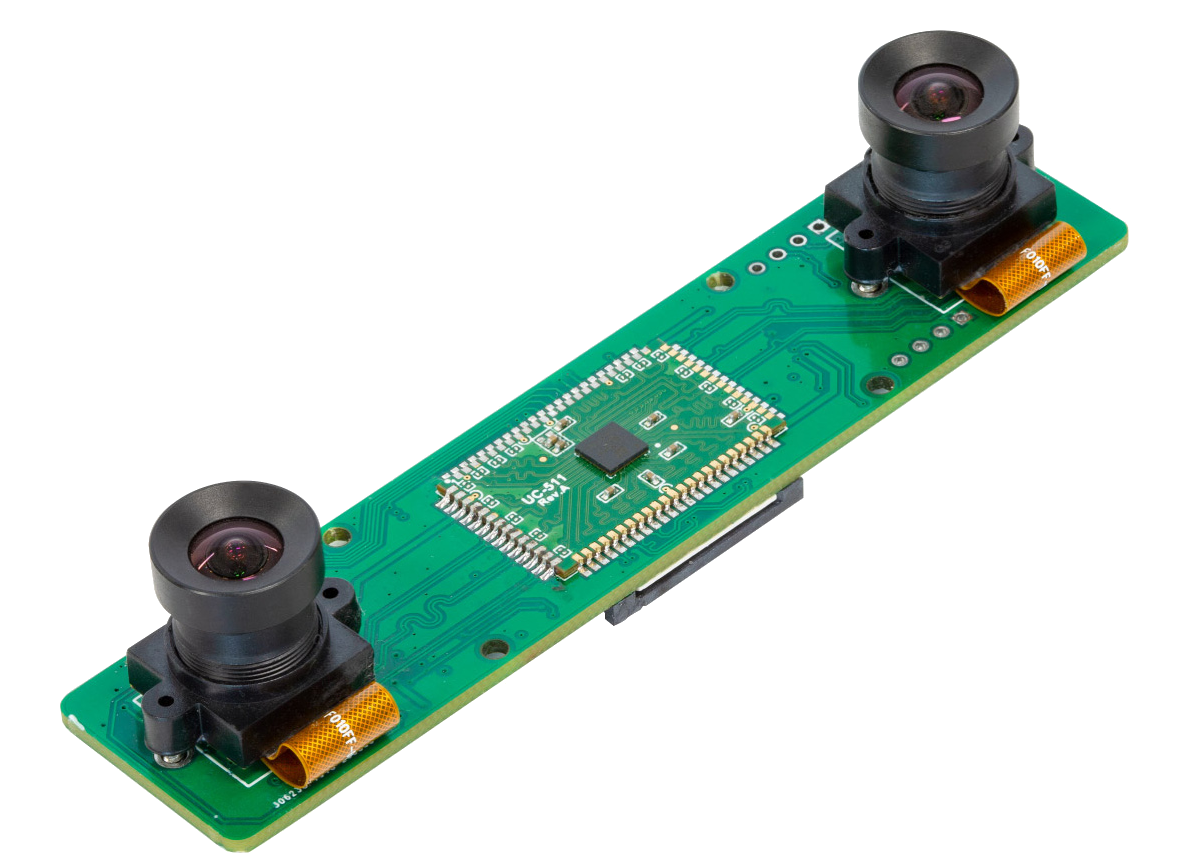
\includegraphics[width=\mythirdmaxsizeimageinsidetable]{chapter5/tablas comparativas/camara estereo 2.png} \\ 
			%\begin{myflushcenter}
			%	{\footnotesize Nombre imagen}
			%\end{myflushcenter}
		\end{minipage}
		&  
		\begin{minipage}{\mythirdmaxsizeofcontenttable}
			\centering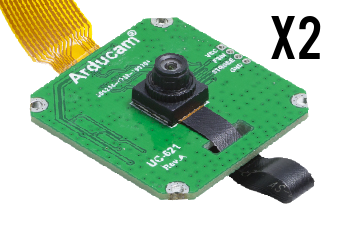
\includegraphics[width=\mythirdmaxsizeimageinsidetable]{chapter5/tablas comparativas/camara estereo 3.png} \\ 
			%\begin{myflushcenter}
			%	{\footnotesize Nombre imagen}
			%\end{myflushcenter}
		\end{minipage}\\ \hline
		\multicolumn{1}{|l|}{
			\begin{minipage}{\myforthmaxsizeofcontenttable}	
				\textbf{Fabricante}
			\end{minipage}
		} & - & OpenCV & ArduCam & ArduCam \\ \hline
		\multicolumn{1}{|l|}{
			\begin{minipage}{\myforthmaxsizeofcontenttable}	
				\textbf{Sensor óptico}
			\end{minipage}
		} & - & OV9282 & OV9281 & OV2311 \\ \hline
		\multicolumn{1}{|l|}{
			\begin{minipage}{\myforthmaxsizeofcontenttable}	
				\textbf{Año de fabricación}
			\end{minipage}
		} & - & 2020 & 2020 & 2019 \\ \hline
		\multicolumn{1}{|l|}{
			\begin{minipage}{\myforthmaxsizeofcontenttable}	
				\textbf{Tipo de obturador}
			\end{minipage}
		} & 
		\begin{minipage}{\mythirdmaxsizeofcontenttable}\begin{myflushcenterinsidetable}
			Global 
		\end{myflushcenterinsidetable}\end{minipage} & 
		\begin{minipage}{\mythirdmaxsizeofcontenttable}\begin{myflushcenterinsidetable}
			Global sincronizado 
		\end{myflushcenterinsidetable}\end{minipage} &
		\begin{minipage}{\mythirdmaxsizeofcontenttable}\begin{myflushcenterinsidetable}
			Global sincronizado 
		\end{myflushcenterinsidetable}\end{minipage}&
		\begin{minipage}{\mythirdmaxsizeofcontenttable}\begin{myflushcenterinsidetable}
			Global dual 
		\end{myflushcenterinsidetable}\end{minipage} \\ \hline
		\multicolumn{1}{|l|}{
			\begin{minipage}{\myforthmaxsizeofcontenttable}	
				\textbf{Escala de colores}
			\end{minipage}
		} & - & B/N HDR & B/N & B/N \\ \hline
		\multicolumn{1}{|l|}{
			\begin{minipage}{\myforthmaxsizeofcontenttable}	
				\textbf{Resolución}
			\end{minipage}
		} & 0.5MP & 
		\begin{minipage}{\mythirdmaxsizeofcontenttable}\begin{myflushcenterinsidetable}
				1MP (1280× 800 $px/3{\mu}m$)
		\end{myflushcenterinsidetable}\end{minipage} & 
		\begin{minipage}{\mythirdmaxsizeofcontenttable}\begin{myflushcenterinsidetable}
				1MP (1280× 800 $px/3{\mu}m$)
		\end{myflushcenterinsidetable}\end{minipage} & 
		\begin{minipage}{\mythirdmaxsizeofcontenttable}\begin{myflushcenterinsidetable}
				2MP (1600x 1300 $px/3{\mu}m$)
		\end{myflushcenterinsidetable}\end{minipage} \\ \hline
		\multicolumn{1}{|l|}{
			\begin{minipage}{\myforthmaxsizeofcontenttable}	
				\textbf{Frames por segundo ($FPS$)}
			\end{minipage}
		} & 50 % NECESITO MÁS DE 80
		& 120 & 60 & 60 \\ \hline
		\multicolumn{1}{|l|}{
			\begin{minipage}{\myforthmaxsizeofcontenttable}	
				\textbf{Tamaño de lente ('')}
			\end{minipage}
		} & Independiente & 1/2.3 & 1/4 & 1/2.9 \\ \hline
		\multicolumn{1}{|l|}{
			\begin{minipage}{\myforthmaxsizeofcontenttable}	
				\textbf{Enfoque ($mm.$)}
			\end{minipage}
		} & - & [196;$\infty$] & [30;$\infty$] & [30;$\infty$] \\ \hline
		\multicolumn{1}{|l|}{
			\begin{minipage}{\myforthmaxsizeofcontenttable}
				\textbf{Campo de visión ° (HFDV,VFDV,DFDV)\footnote{HFDV: Campo de visión horizontal. VFDV: Campo de visión vertical. DFDV: Campo de visión diagonal}}
			\end{minipage}
		} & Adaptable & 71.8, --, 81.0 & 70, 52.1 , -- & 100, 68.2, -- \\ \hline
		\multicolumn{1}{|l|}{
			\begin{minipage}{\myforthmaxsizeofcontenttable}	
				\textbf{Procesamiento gráfico}
			\end{minipage}
		} & - & MA2085 VPU\footnote{Movidius™ Myriad™ VPU. \href{https://www.intel.com/content/www/us/en/products/processors/movidius-vpu/movidius-myriad-x.html}{Enlace a unidad de procesamiento de visión.}} & 
		\begin{minipage}{\mythirdmaxsizeofcontenttable}\begin{myflushcenterinsidetable}
			Jetson Nano o Xavier NX
		\end{myflushcenterinsidetable}\end{minipage}
	 	& \begin{minipage}{\mythirdmaxsizeofcontenttable}\begin{myflushcenterinsidetable}
	 			Raspberry Pi 3
	 	\end{myflushcenterinsidetable}\end{minipage} \\ \hline 
	 	\multicolumn{1}{|l|}{
	 		\begin{minipage}{\myforthmaxsizeofcontenttable}	
	 			\textbf{Temperatura operativa}
	 		\end{minipage}
	 	} & [-10;50] & [-30;60] & [-30;85] & [-30;85] \\ \hline
		\multicolumn{1}{|l|}{
			\begin{minipage}{\myforthmaxsizeofcontenttable}	
				\textbf{Soporte IA\footnote{Chips diseñados y optimizados para procesar detección de objetos mediante redes neuronales.}}
			\end{minipage}
		} & - & Sí & Sí & No \\ \hline
		\multicolumn{1}{|l|}{
			\begin{minipage}{\myforthmaxsizeofcontenttable}	
				\textbf{Consumo de energía ($W$)}
			\end{minipage}
		} & <10 & $\approx4$ & - & - \\ \hline
		\multicolumn{1}{|l|}{
			\begin{minipage}{\myforthmaxsizeofcontenttable}	
				\textbf{Precio (S/)}
			\end{minipage}
		} & <1000 & 475.41 & 358.97 & 717.28 \\ \hline
	\end{tabular}
	\begin{myflushcenteraftertable}	
		Fuente: OpenCV, ArduCam y elaboración propia. Hoja de datos técnica (\textit{Datasheet}) en el Anexo.\\
		Tasa de cambio de USD a PEN: S/ 3.59.
	\end{myflushcenteraftertable}
\end{mytable}
\end{savenotes}

La cámara escogida es la OAK-D debido a que cuenta con un sistema de obturación Global sincronizado\footnote{Superior al sincronizado dual para la tarea en el sistema.}, aunque el requerimiento mínimo de cuadros por segundo es de 50, en la práctica se requiere que el sistema no trabaje a sus máxima capacidad y el aporte que brinda el procesamiento en el mismo dispositivo que evita sobrecargar el servidor.

%% NUEVO SECCION X.X.X.
\subsection{Selección de cámara simple}
	
La cámara simple tiene como función verificar la correcta trayectoria de las truchas en el mecanismo de distribución hacia las respectivas jaulas flotantes. Los requerimientos técnicos se presentan en la Tabla \ref{tab:tabla comparativa de camaras simples} así como las principales características de cada una.

\begin{savenotes}
	\begin{mytable}[H]
		\footnotesize\centering
		\caption{Tabla comparativa de cámaras.}
		\label{tab:tabla comparativa de camaras simples}
		\begin{tabular}{l|c|c|c|c|}
			\cline{2-5}
			\multicolumn{1}{c|}{\textbf{}}            & \textbf{\begin{tabular}[c]{@{}c@{}}Requisitos\\ mínimos\end{tabular}} & 
			\multicolumn{1}{|l|}{				
				\begin{minipage}{\mythirdmaxsizeofcontenttable}
					\begin{myflushcenterinsidetable}
						\textbf{B0249}
					\end{myflushcenterinsidetable}
				\end{minipage}
			}&
			\multicolumn{1}{|l|}{				
				\begin{minipage}{\mythirdmaxsizeofcontenttable}	
					\begin{myflushcenterinsidetable}
						\textbf{Alvium 1800 U-500m}
					\end{myflushcenterinsidetable}
				\end{minipage}
			}&
			%\multicolumn{1}{|l|}{				
			%	\begin{minipage}{\mythirdmaxsizeofcontenttable}	
			%		\begin{myflushcenter}
			%			\textbf{CMT-8MP- IMX219M366}
			%		\end{myflushcenter}
			%	\end{minipage}
			%}  
			\multicolumn{1}{|l|}{				
				\begin{minipage}{\mythirdmaxsizeofcontenttable}	
					\begin{myflushcenterinsidetable}
						\textbf{OAK-1}
					\end{myflushcenterinsidetable}
				\end{minipage}
			}  \\ \hline
			\multicolumn{1}{|l|}{\textbf{Figura}} & - 
			&		  
			\begin{minipage}{\mythirdmaxsizeofcontenttable}
				\centering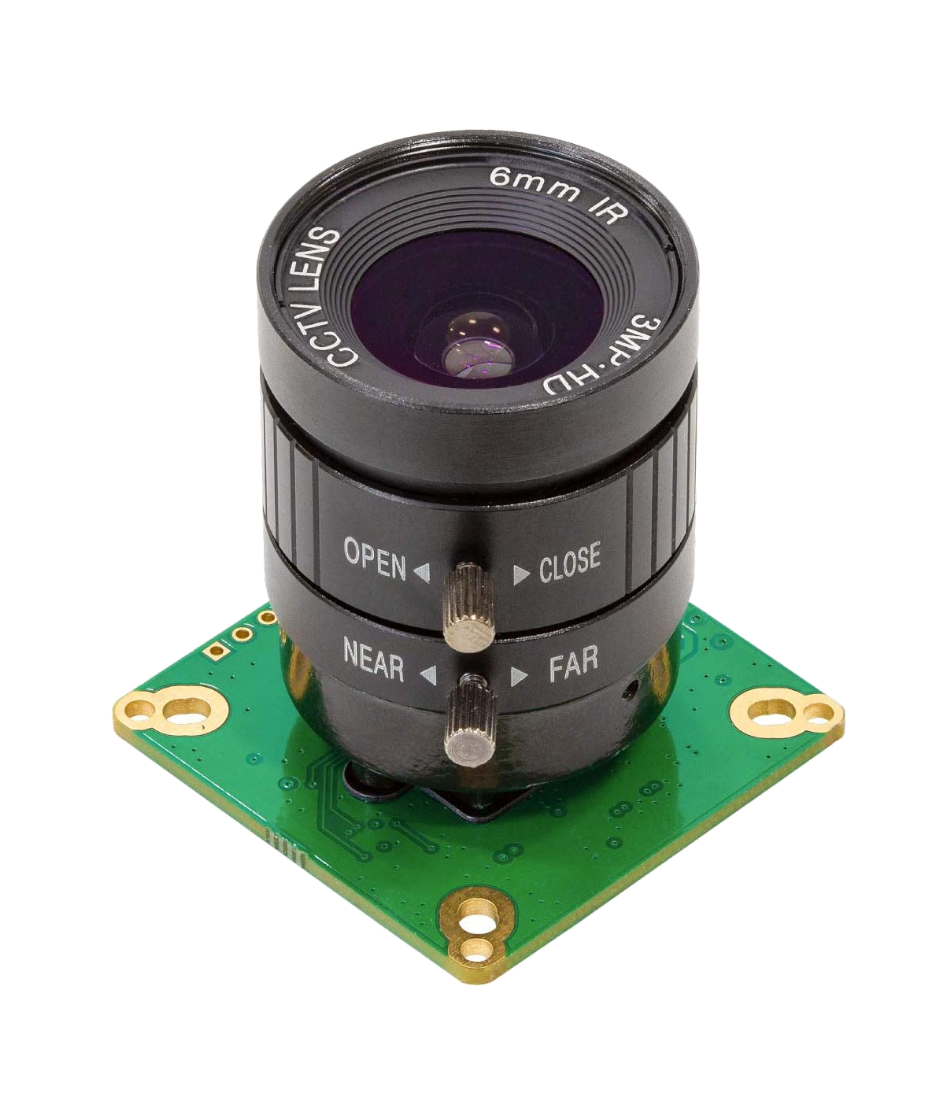
\includegraphics[width=\mythirdmaxsizeimageinsidetable]{chapter5/tablas comparativas/camara simple 1.png} \\ 
				%\begin{myflushcenter}
				%	{\footnotesize Nombre imagen}
				%\end{myflushcenter}
			\end{minipage}
			&		  
			\begin{minipage}{\mythirdmaxsizeofcontenttable}
				\centering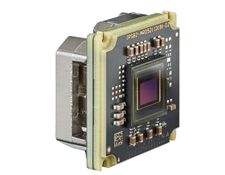
\includegraphics[width=\mythirdmaxsizeimageinsidetable]{chapter5/tablas comparativas/camara simple 2.png} \\ 
				%\begin{myflushcenter}
				%	{\footnotesize Nombre imagen}
				%\end{myflushcenter}
			\end{minipage}
			&  
			\begin{minipage}{\mythirdmaxsizeofcontenttable}
				\centering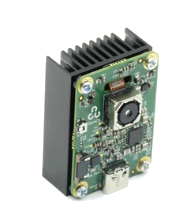
\includegraphics[width=\mythirdmaxsizeimageinsidetable]{chapter5/tablas comparativas/camara simple 4.png} \\ 
				%\begin{myflushcenter}
				%	{\footnotesize Nombre imagen}
				%\end{myflushcenter}
			\end{minipage}\\ \hline
			\multicolumn{1}{|l|}{
				\begin{minipage}{\myforthmaxsizeofcontenttable}	
					\textbf{Fabricante}
				\end{minipage}
			} & - & ArduCam & Allied Vision & ArduCam \\ \hline
			\multicolumn{1}{|l|}{
				\begin{minipage}{\myforthmaxsizeofcontenttable}	
					\textbf{Sensor óptico}
				\end{minipage}
			} & - & IMX477  & 
			\begin{minipage}{\mythirdmaxsizeofcontenttable}\begin{myflushcenterinsidetable}
					ON Semi AR0521SR
			\end{myflushcenterinsidetable}\end{minipage} & 
			%IMX219 
			IMX378
			\\ \hline
			\multicolumn{1}{|l|}{
				\begin{minipage}{\myforthmaxsizeofcontenttable}	
					\textbf{Año de fabricación}
				\end{minipage}
			} & - & 2020 & 2019 & 2020 \\ \hline
			\multicolumn{1}{|l|}{
				\begin{minipage}{\myforthmaxsizeofcontenttable}	
					\textbf{Tipo de obturador}
				\end{minipage}
			} & 
			\begin{minipage}{\mythirdmaxsizeofcontenttable}\begin{myflushcenterinsidetable}
					- 
			\end{myflushcenterinsidetable}\end{minipage} & 
			\begin{minipage}{\mythirdmaxsizeofcontenttable}\begin{myflushcenterinsidetable}
					Global
			\end{myflushcenterinsidetable}\end{minipage} &
			\begin{minipage}{\mythirdmaxsizeofcontenttable}\begin{myflushcenterinsidetable}
					Rolling 
			\end{myflushcenterinsidetable}\end{minipage}&
			%\begin{minipage}{\mythirdmaxsizeofcontenttable}\begin{myflushcenterinsidetable}
			%		Rolling 
			%\end{myflushcenterinsidetable}\end{minipage} 
			\begin{minipage}{\mythirdmaxsizeofcontenttable}\begin{myflushcenterinsidetable}
				Global 
			\end{myflushcenterinsidetable}\end{minipage} 			
			\\ \hline
			\multicolumn{1}{|l|}{
				\begin{minipage}{\myforthmaxsizeofcontenttable}	
					\textbf{Escala de colores}
				\end{minipage}
			} & - & RGB & B/N & RGB \\ \hline
			\multicolumn{1}{|l|}{
			\begin{minipage}{\myforthmaxsizeofcontenttable}	
				\textbf{Resolución}
			\end{minipage}
			} & 0.5MP & 
			\begin{minipage}{\mythirdmaxsizeofcontenttable}\begin{myflushcenterinsidetable}
				12.3MP (4056× 3040 $px/1.55{\mu}m$)
			\end{myflushcenterinsidetable}\end{minipage} & 
			\begin{minipage}{\mythirdmaxsizeofcontenttable}\begin{myflushcenterinsidetable}
				5MP (2592x 1944 $px/2.2{\mu}m$)
			\end{myflushcenterinsidetable}\end{minipage} & 
			%\begin{minipage}{\mythirdmaxsizeofcontenttable}\begin{myflushcenterinsidetable}
			%	8MP (3280x 2464 $px/1.12{\mu}m$)
			%\end{myflushcenterinsidetable}\end{minipage} 
			\begin{minipage}{\mythirdmaxsizeofcontenttable}\begin{myflushcenterinsidetable}
				12MP (4056× 3040 $px/1.55{\mu}m$)
			\end{myflushcenterinsidetable}\end{minipage} 
			\\ \hline
			\multicolumn{1}{|l|}{
			\begin{minipage}{\myforthmaxsizeofcontenttable}	
				\textbf{Frames por segundo ($FPS$)}
			\end{minipage}
			} & 40 % NECESITO MÁS DE 80
			& 60 & 67 & 
			%720p60 
			60
			\\ \hline
			\multicolumn{1}{|l|}{
			\begin{minipage}{\myforthmaxsizeofcontenttable}	
				\textbf{Tamaño de lente ('')}
			\end{minipage}
			} & Independiente & 1/2.3 & 1/2.5 &
			% 1/4
			1/2.3
			\\ \hline
			\multicolumn{1}{|l|}{
			\begin{minipage}{\myforthmaxsizeofcontenttable}
				\textbf{Campo de visión ° (HFDV,VFDV,DFDV)\footnote{HFDV: Campo de visión horizontal. VFDV: Campo de visión vertical. DFDV: Campo de visión diagonal}}
			\end{minipage}
			} & Adaptable & 65.0, --, -- & -- & 
			%70, 70, -- 
			71.8, --, 81.0
			\\ \hline
			\multicolumn{1}{|l|}{
			\begin{minipage}{\myforthmaxsizeofcontenttable}	
				\textbf{Procesamiento gráfico}
			\end{minipage}
			} & - & 
			\begin{minipage}{\mythirdmaxsizeofcontenttable}\begin{myflushcenterinsidetable}
				Jetson Nano o Xavier NX
			\end{myflushcenterinsidetable}\end{minipage} & 
			\begin{minipage}{\mythirdmaxsizeofcontenttable}\begin{myflushcenterinsidetable}
				Jetson Nano o Xavier NX
			\end{myflushcenterinsidetable}\end{minipage}&
			%\begin{minipage}{\mythirdmaxsizeofcontenttable}\begin{myflushcenterinsidetable}
			%	Raspberry Pi 3
			%\end{myflushcenterinsidetable}\end{minipage}
			\begin{minipage}{\mythirdmaxsizeofcontenttable}\begin{myflushcenterinsidetable}
				MA2085 VPU\footnote{Movidius™ Myriad™ VPU. \href{https://www.intel.com/content/www/us/en/products/processors/movidius-vpu/movidius-myriad-x.html}{Enlace a unidad de procesamiento de visión.}}
			\end{myflushcenterinsidetable}\end{minipage}  \\ \hline 
			\multicolumn{1}{|l|}{
			\begin{minipage}{\myforthmaxsizeofcontenttable}	
				\textbf{Temperatura operativa}
			\end{minipage}
			} & [-10;50] & [-20;60] & [5;80] & 
			%[-20;70]
         [-30;60]
         \\ \hline
			\multicolumn{1}{|l|}{
			\begin{minipage}{\myforthmaxsizeofcontenttable}	
				\textbf{Consumo de energía ($W$)}
			\end{minipage}
			} & <5 & - & [$\approx$2.2;$\approx$2.4] & 
			%- 
			$\approx$2
			\\ \hline
			\multicolumn{1}{|l|}{
			\begin{minipage}{\myforthmaxsizeofcontenttable}	
				\textbf{Precio (S/)}
			\end{minipage}
			} & <500 & 196.81 & 595.7 & %717.28 
			355.41
			\\ \hline
			\end{tabular}
		\begin{myflushcenteraftertable}	
			Fuente: Allied Vision, ArduCam y elaboración propia. Hoja de datos técnica (\textit{Datasheet}) en el Anexo.\\
			Tasa de cambio de USD a PEN: S/ 3.59.
		\end{myflushcenteraftertable}
	\end{mytable}
\end{savenotes}

La cámara simple escogida es OAK-1 debido a que presenta un tipo de obturador global, un campo de visión mayor a las demás, un procesador gráfico especializado en imágenes y un menor consumo de potencia comparado con las otras opciones.

%% NUEVO SECCION X.X.
\section{Selección de iluminación adecuada} 

La captura de imágenes con los sensores IMX378 y OV9282 están diseñados para ser usados en interiores como en exteriores. Sin embargo, la velocidad de obturación de un cuadro de imagen varía dependiendo de la luz que recibe el sensor. Con el fin de minimizar los riesgos, el control de la luz será parte del sistema y el subsistema correspondiente aislado de la luz natural. La luz artificial controlada por el microprocesador escogido. Además, será necesario una iluminación mínima de 500 luxes ($I_{min}=500$).\footnote{Selección de iluminación: \cite{Ryer1997}.}

El propósito de los LEDs de alta potencia es iluminar la zona en la que se realiza la captura de imágenes para detectar truchas y procesarlas. El uso de una led adecuado, con la iluminación mencionada o mayor, puede mejorar el rendimiento de la cámara. En la Figura \ref{fig:iluminacion opciones} se muestra las opciones de iluminación que se consideraron, resultando el uso de dos tiras de LEDs adecuadas para el sistema debido a la distribución uniforme de luz.\footnote{Se requieren más estudios con el proyecto final para obtener de forma definitiva un diseño. La propuesta no pretende ser la solución óptima sino una adecuada acorde a los requerimientos del sistema en cuestión.}

% EN LA CARPETA IMAGENES ESTAN TODA LAS IMAGENES BASE
\begin{myfigure}[H]
	\footnotesize\centering
	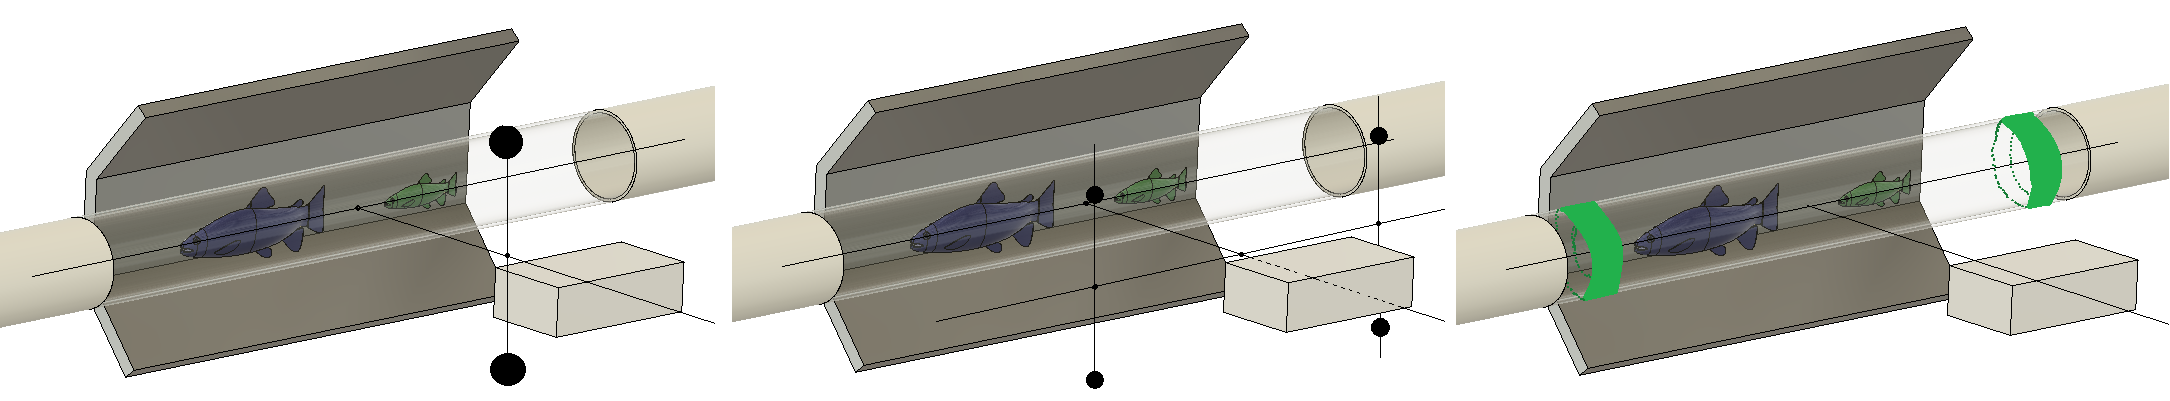
\includegraphics[width=1\textwidth]{chapter5/iluminacion opciones.png}
	\caption[Opciones de posicionamiento de iluminación.]{(Izq.) Iluminación con dos LEDs frente al sistema. (Cen.) Iluminación con cuatro LEDs frente al sistema. (Der.) Iluminación con dos tiras LEDs.}
	\begin{myflushcenter}
		Fuente: Elaboración propia.
	\end{myflushcenter}
	\label{fig:iluminacion opciones}
\end{myfigure}

En la Tabla \ref{tab:tabla comparativa de leds de alta potencia} se muestra una tabla técnica comparativa de tres opciones de tiras de leds de alta potencia, ya que de esta forma se presentan comercialmente. En dicha Tabla, se observa que la presentación ($m.$) varía según la marca.

\begin{savenotes}
	\begin{mytable}[H]
		\footnotesize\centering
		\caption{Tabla comparativa de leds de alta potencia.}
		\label{tab:tabla comparativa de leds de alta potencia}
		\begin{tabular}{l|c|c|c|c|}
			\cline{2-5}
			\multicolumn{1}{c|}{\textbf{}}& \textbf{\begin{tabular}[c]{@{}c@{}}Requisitos\\ mínimos\end{tabular}} & 
			\multicolumn{1}{|l|}{				
				\begin{minipage}{\mythirdmaxsizeofcontenttable}\begin{myflushcenterinsidetable}
						\textbf{JED-LS12V/ T20/ 120/ 5}
				\end{myflushcenterinsidetable}\end{minipage}
			}&
			\multicolumn{1}{|l|}{				
				\begin{minipage}{\mythirdmaxsizeofcontenttable}\begin{myflushcenterinsidetable}
						\textbf{PSH601A/ PSH602A}
				\end{myflushcenterinsidetable}\end{minipage}
			}&
			\multicolumn{1}{|l|}{				
				\begin{minipage}{\mythirdmaxsizeofcontenttable}\begin{myflushcenterinsidetable}
						\textbf{PSB602Z}
				\end{myflushcenterinsidetable}\end{minipage}
			}  \\ \hline
			\multicolumn{1}{|l|}{\textbf{Figura}} & - 
			&		  
			\begin{minipage}{\mythirdmaxsizeofcontenttable}
				\centering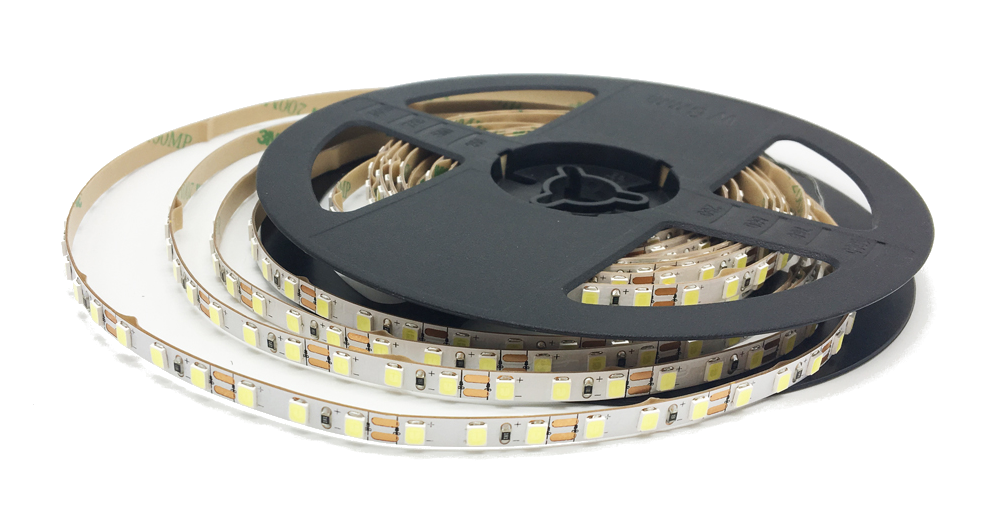
\includegraphics[width=\mythirdmaxsizeimageinsidetable]{chapter5/tablas comparativas/led alta potencia 1.png} \\ 
				%\begin{myflushcenter}
				%	{\footnotesize Nombre imagen}
				%\end{myflushcenter}
			\end{minipage}
			&		  
			\begin{minipage}{\mythirdmaxsizeofcontenttable}
				\centering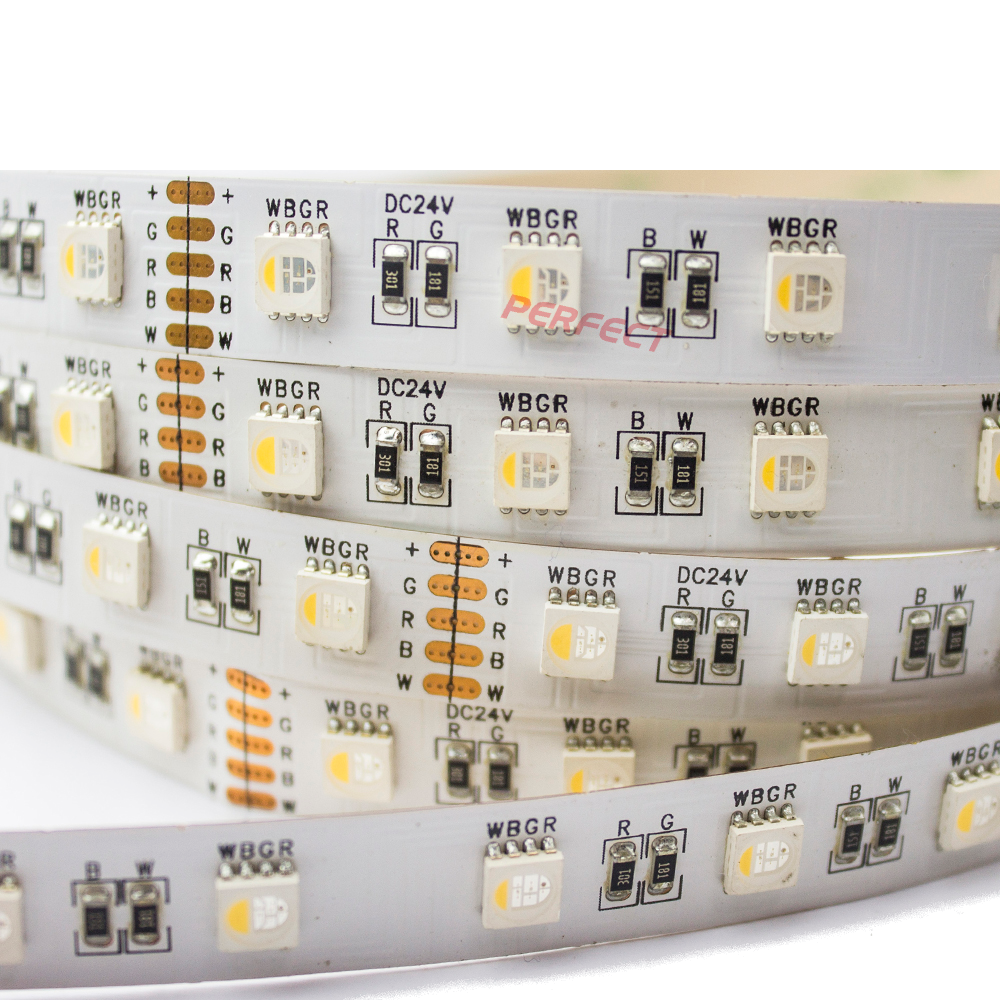
\includegraphics[width=\mythirdmaxsizeimageinsidetable]{chapter5/tablas comparativas/led alta potencia 2.png} \\ 
				%\begin{myflushcenter}
				%	{\footnotesize Nombre imagen}
				%\end{myflushcenter}
			\end{minipage}
			&  
			\begin{minipage}{\mythirdmaxsizeofcontenttable}
				\centering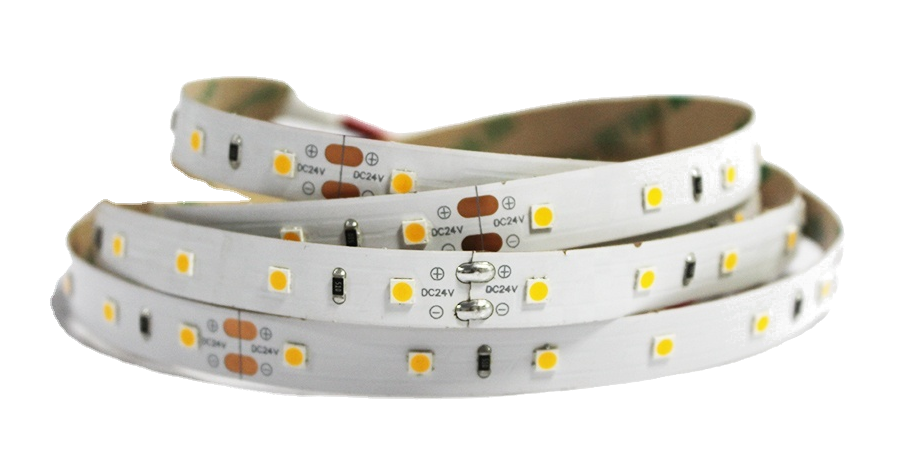
\includegraphics[width=\mythirdmaxsizeimageinsidetable]{chapter5/tablas comparativas/led alta potencia 3.png} \\ 
				%\begin{myflushcenter}
				%	{\footnotesize Nombre imagen}
				%\end{myflushcenter}
			\end{minipage}\\ \hline
			\multicolumn{1}{|l|}{
				\begin{minipage}{\myforthmaxsizeofcontenttable}	
					\textbf{Fabricante}
				\end{minipage}
			} & - & JEDVER & NICHIA & PERFECT \\ \hline	
			\multicolumn{1}{|l|}{
				\begin{minipage}{\myforthmaxsizeofcontenttable}	
					\textbf{Potencia de LED ($W/m$)}
				\end{minipage}
			} & - & 9.6 & 14.4 & 18 \\ \hline
			\multicolumn{1}{|l|}{
				\begin{minipage}{\myforthmaxsizeofcontenttable}	
					\textbf{Temperatura operativa (°$C$)}
				\end{minipage}
			} & [-10; 40] & [-20; 50] & [-20; 45] & [-20; 45] \\ \hline
			\multicolumn{1}{|l|}{
				\begin{minipage}{\myforthmaxsizeofcontenttable}	
					\textbf{Eficacia luminosa ($lm/W$)}
				\end{minipage}
			} & >70 & 80 & - & 75 \\ \hline
			\multicolumn{1}{|l|}{
				\begin{minipage}{\myforthmaxsizeofcontenttable}	
					\textbf{Flujo luminoso por metro ($lm/m$)}
				\end{minipage}
			} & >500 & 10.2 & 20 & 60-65 \\ \hline
			\multicolumn{1}{|l|}{
				\begin{minipage}{\myforthmaxsizeofcontenttable}	
					\textbf{Material principal}
				\end{minipage}
			} & - & FPC & Cobre & Cobre \\ \hline
			\multicolumn{1}{|l|}{
				\begin{minipage}{\myforthmaxsizeofcontenttable}	
					\textbf{Fuente de luz LED}
				\end{minipage}
			} & - & SMD2016 & SMD5050 & SMD3030 \\ \hline
			\multicolumn{1}{|l|}{
				\begin{minipage}{\myforthmaxsizeofcontenttable}	
					\textbf{Nivel de protección ($IP$)}
				\end{minipage}
			} & - & [IP20; IP65] & [IP20; IP68] & [IP20; IP68] \\ \hline
			\multicolumn{1}{|l|}{
				\begin{minipage}{\myforthmaxsizeofcontenttable}	
					\textbf{Voltaje de consumo ($V$)}
				\end{minipage}
			} & - & 12/24 & 12/24 & 24 \\ \hline
			\multicolumn{1}{|l|}{
				\begin{minipage}{\myforthmaxsizeofcontenttable}	
					\textbf{Cantidad de leds ($LEDs/m$)}
				\end{minipage}
			} & - & 60 & 60 & 60 \\ \hline
			\multicolumn{1}{|l|}{
				\begin{minipage}{\myforthmaxsizeofcontenttable}	
					\textbf{Temperatura de color ($K$)}
				\end{minipage}
			} & - & [2700; 6500] & [2700; 6000] & [2700; 6500] \\ \hline
			\multicolumn{1}{|l|}{
				\begin{minipage}{\myforthmaxsizeofcontenttable}	
					\textbf{Tiempo de vida útil ($h$)}
				\end{minipage}
			} & >10000 & 50000 & 35000 & 30000 \\ \hline
			\multicolumn{1}{|l|}{
				\begin{minipage}{\myforthmaxsizeofcontenttable}	
					\textbf{Presentación comercial ($m$)}
				\end{minipage}
			} & - & 50 & 10 & 20 \\ \hline
			\multicolumn{1}{|l|}{
				\begin{minipage}{\myforthmaxsizeofcontenttable}	
					\textbf{Precio por metro ($S/$)}
				\end{minipage}
			} & - & 3.95 & 17.23 & 26.93 \\ \hline
		\end{tabular}
		\begin{myflushcenteraftertable}	
			Fuente: Imágenes de dominio público y elaboración propia. Hoja de datos técnica (\textit{Datasheet}) en el Anexo.\\
			Tasa de cambio de USD a PEN: S/ 3.59.
		\end{myflushcenteraftertable}
	\end{mytable}
\end{savenotes}

El modelo escogido es el PSH6012A ya que tiene una presentación menor y cumple con el flujo luminoso, además de presentar protección al agua ($IP68$) y aunque el consumo de potencia es mayor, tiene un menor costo comparado con la adquisición de otras marcas. Finalmente, mencionar que el precio total sería de S/ 170.23, aunque se puede adquirir por metros en el comercio nacional.

%% NUEVO SECCION X.X.
\section{Selección de sensor de luz}

Al sensar la luz, se establece un espectro de frecuencia a ser medido, en el presente caso se define como requerimiento el sensado de luz digital de un determinado rango en cuanto a la intensidad y frecuencias. En la Tabla \ref{tab:tabla comparativa sensores de iluminación} se comparan dispositivos que cumplen con los requerimientos mínimos.

\begin{savenotes}
	\begin{mytable}[H]
		\footnotesize\centering
		\caption{Tabla comparativa de sensores de iluminación.}
		\label{tab:tabla comparativa sensores de iluminación}
		\begin{tabular}{l|c|c|c|c|}
			\cline{2-5}
			\multicolumn{1}{c|}{\textbf{}}& \textbf{\begin{tabular}[c]{@{}c@{}}Requisitos\\ mínimos\end{tabular}} & 
			\multicolumn{1}{|l|}{				
				\begin{minipage}{\mythirdmaxsizeofcontenttable}\begin{myflushcenterinsidetable}
						\textbf{SI1445}
				\end{myflushcenterinsidetable}\end{minipage}
			}&
			\multicolumn{1}{|l|}{				
				\begin{minipage}{\mythirdmaxsizeofcontenttable}\begin{myflushcenterinsidetable}
						\textbf{TSL2561}
				\end{myflushcenterinsidetable}\end{minipage}
			}&
			\multicolumn{1}{|l|}{				
				\begin{minipage}{\mythirdmaxsizeofcontenttable}\begin{myflushcenterinsidetable}
						\textbf{VCNL4010}
				\end{myflushcenterinsidetable}\end{minipage}
			}  \\ \hline
			\multicolumn{1}{|l|}{\textbf{Figura}} & - 
			&		  
			\begin{minipage}{\mythirdmaxsizeofcontenttable}
				\centering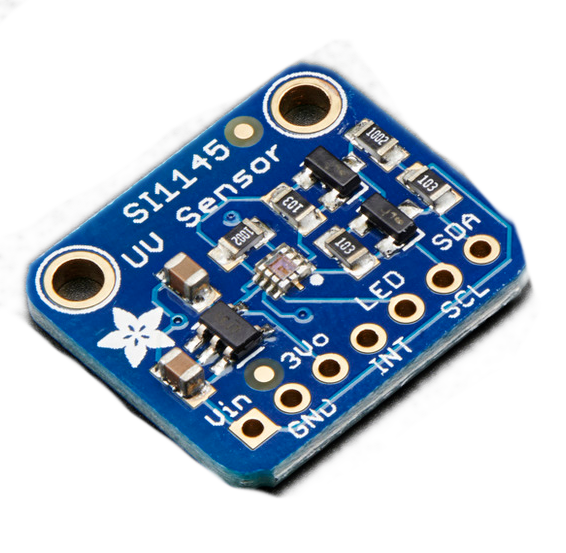
\includegraphics[width=\mythirdmaxsizeimageinsidetable]{chapter5/tablas comparativas/sensor luz 1.png} \\ 
				%\begin{myflushcenter}
				%	{\footnotesize Nombre imagen}
				%\end{myflushcenter}
			\end{minipage}
			&		  
			\begin{minipage}{\mythirdmaxsizeofcontenttable}
				\centering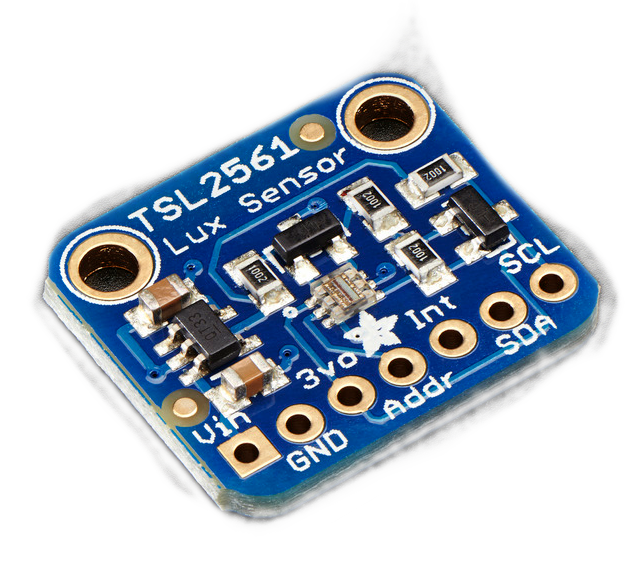
\includegraphics[width=\mythirdmaxsizeimageinsidetable]{chapter5/tablas comparativas/sensor luz 2.png} \\ 
				%\begin{myflushcenter}
				%	{\footnotesize Nombre imagen}
				%\end{myflushcenter}
			\end{minipage}
			&  
			\begin{minipage}{\mythirdmaxsizeofcontenttable}
				\centering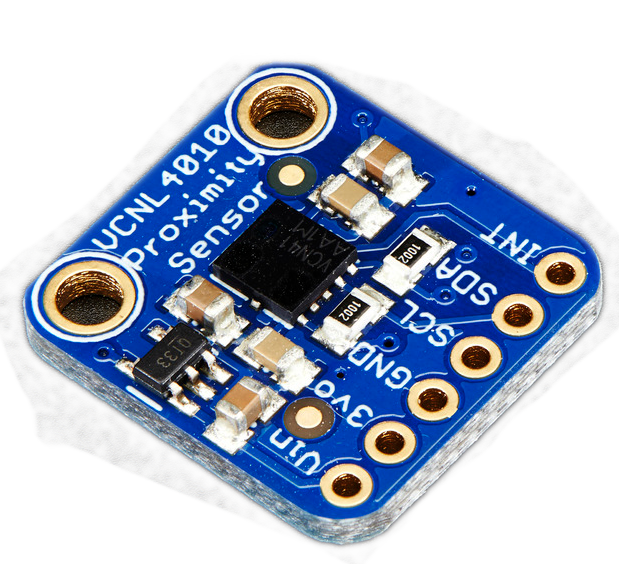
\includegraphics[width=\mythirdmaxsizeimageinsidetable]{chapter5/tablas comparativas/sensor luz 3.png} \\ 
				%\begin{myflushcenter}
				%	{\footnotesize Nombre imagen}
				%\end{myflushcenter}
			\end{minipage}\\ \hline
			\multicolumn{1}{|l|}{
				\begin{minipage}{\myforthmaxsizeofcontenttable}	
					\textbf{Fabricante}
				\end{minipage}
			} & - & Adafruit & Adafruit & Adafruit \\ \hline
			\multicolumn{1}{|l|}{
				\begin{minipage}{\myforthmaxsizeofcontenttable}	
					\textbf{Protocolo de comunicación}
				\end{minipage}
			} & - & I2C & I2C & I2C \\ \hline
			\multicolumn{1}{|l|}{
				\begin{minipage}{\myforthmaxsizeofcontenttable}	
					\textbf{Voltaje operativo ($V$)}
				\end{minipage}
			} & [0; 5] & [1.71; 3.6] & [2.7; 3.6] & [2.5; 3.6] \\ \hline
			\multicolumn{1}{|l|}{
				\begin{minipage}{\myforthmaxsizeofcontenttable}	
					\textbf{Temperatura operativa (°$C$)}
				\end{minipage}
			} & [-10; 40] & [-40; 85] & [-30; 70] & [-25; 85] \\ \hline
			\multicolumn{1}{|l|}{
			\begin{minipage}{\myforthmaxsizeofcontenttable}	
				\textbf{Rango de medición ($lx$)}
			\end{minipage}
			} & [0; 20000] & [0; 40000] & [0; 40000] & [0; 45000] \\ \hline
			\multicolumn{1}{|l|}{
				\begin{minipage}{\myforthmaxsizeofcontenttable}	
					\textbf{Resolución ADC ($bit$)}
				\end{minipage}
			} & - & 16 & 16 & 16 \\ \hline
			\multicolumn{1}{|l|}{
				\begin{minipage}{\myforthmaxsizeofcontenttable}	
					\textbf{Resolución digital ($lx$)}
				\end{minipage}
			} & 100 & 0.10 & 0.11 & 0.25 \\ \hline
			\multicolumn{1}{|l|}{
				\begin{minipage}{\myforthmaxsizeofcontenttable}	
					\textbf{Precio ($S/$)}
				\end{minipage}
			} & - & 35.72 & 21.36 & 26.92 \\ \hline
		\end{tabular}
		\begin{myflushcenteraftertable}	
			Fuente: Imágenes de dominio público y elaboración propia. Hoja de datos técnica (\textit{Datasheet}) en el Anexo.\\
			Tasa de cambio de USD a PEN: S/ 3.59.
		\end{myflushcenteraftertable}
	\end{mytable}
\end{savenotes}

Se elige el sensor de luz con código TSL2561 debido a que satisface los requerimientos mínimos y presenta un precio inferior a los contrarios. Además, recalcar que el estudio no requiere un sensor de alta precisión sino uno que permita un adecuado funcionamiento del subsistema de procesamiento de imágenes.

%% NUEVO SECCION X.X.
\section{Selección de algoritmo de clasificación y conteo}
\label{sssec:seleccion de algoritmo de clasificacion y conteo}

Existen diversas tecnologías para la clasificación y conteo\footnote{Detallado en \textit{"Estado del Arte"} de \cite{DiazVergara2020}.}, en el presente trabajo se escoge e implementa redes neuronales. Los algoritmos de detección de objecto se dividen en sectores dependiendo de la aplicación: \href{https://paperswithcode.com/sota/real-time-object-detection-on-coco}{tiempo-real}, \href{https://paperswithcode.com/sota/object-detection-on-coco}{post procesamiento} y para \href{https://paperswithcode.com/sota/3d-object-detection-on-kitti-cars-moderate}{imágenes 3D}. Emplearemos el procesamiento en tiempo real para evitar un post-procesamiento. En la Tabla \ref{tab:tabla comparativa de algoritmos} se presenta una comparación técnica de la cantidad máxima de fotogramas, MAP\footnote{ \textit{(Max Average Precision).} Precisión máxima promedio hace referencia a la precisión obtenida en condiciones que permiten usar el modelo a la mayor cantidad de fotogramas.} y el tiempo de inferencia ($t_{inf}$) en milisegundos. Además, se adjunta la fecha de publicación de los modelos ya que este sector está evolucionando de manera rápida\footnote{Los modelos propuestos por investigadores usualmente son de libre uso, las tecnologías son de código abierto.}.

\begin{myfigure}[H]
	\footnotesize\centering
	\includegraphics[width=1\textwidth]{chapter5/real time object detection.png}
	\caption{Comparación entre modelos de redes neuronales de detección de objetos en tiempo real usando el dataset "COCO".}
	\begin{myflushcenter}
		Fuente: Elaboración propia.
	\end{myflushcenter}
	\label{fig:real time object detection}
\end{myfigure}

En la Tabla \ref{tab:tabla comparativa de algoritmos} se lista los diez modelos de redes neuronales junto con el \textit{paper}, el \textit{código}, el año en que fueron publicado y otras características técnicas. Estos modelos fueron ordenados de mayor a menor en cuanto a fotogramas obtenidos. Con el fin de obtener más fotogramas, se suele re-dimensionar las imágenes a procesar\footnote{Usualmente a imágenes cuadras de  128,256,512 px.}.

\begin{savenotes}
	\begin{mytable}[H]
		\footnotesize\centering
		\caption{Tabla comparativa de algoritmos de detección de objetos en tiempo real ordenados por cantidad de fotogramas máximos obtenidos.}
		\label{tab:tabla comparativa de algoritmos}
		\begin{tabular}{|c|l|c|c|c|l|c|c|}
			\hline
			{\color[HTML]{000000} \textbf{Puesto}} & \multicolumn{1}{c|}{{\color[HTML]{000000} \textbf{\begin{tabular}[c]{@{}c@{}}Nombre de \\ modelo\end{tabular}}}} & {\color[HTML]{000000} \textbf{MAP}} & {\color[HTML]{000000} \textbf{fps}} & {\color[HTML]{000000} \textbf{$t_{inf}$}} & \multicolumn{1}{c|}{{\color[HTML]{000000} \textbf{Nombre de paper}}} & {\color[HTML]{000000} \textbf{\begin{tabular}[c]{@{}c@{}}Paper y\\ Código\end{tabular}}} & {\color[HTML]{000000} \textbf{Año}} \\ \hline
			{\color[HTML]{000000} \textbf{1}} & {\color[HTML]{000000} YOLOv4-512} & {\color[HTML]{000000} 43} & {\color[HTML]{000000} 83} & {\color[HTML]{000000} 12} & {\color[HTML]{000000} \begin{tabular}[c]{@{}l@{}}YOLOv4: Optimal Speed and \\ Accuracy of Object Detection 512\end{tabular}} & {\color[HTML]{000000} \href{https://paperswithcode.com/paper/yolov4-optimal-speed-and-accuracy-of-object}{P} \href{https://paperswithcode.com/paper/yolov4-optimal-speed-and-accuracy-of-object#code}{C}} & {\color[HTML]{000000} 2020} \\ \hline
			{\color[HTML]{000000} \textbf{2}} & {\color[HTML]{000000} YOLOv4-608} & {\color[HTML]{000000} 43.5} & {\color[HTML]{000000} 62} & {\color[HTML]{000000} 16} & {\color[HTML]{000000} \begin{tabular}[c]{@{}l@{}}YOLOv4: Optimal Speed and \\ Accuracy of Object Detection 608\end{tabular}} & {\color[HTML]{000000} \href{https://paperswithcode.com/paper/yolov4-optimal-speed-and-accuracy-of-object}{P} \href{https://paperswithcode.com/paper/yolov4-optimal-speed-and-accuracy-of-object#code}{C}} & {\color[HTML]{000000} 2020} \\ \hline
			{\color[HTML]{000000} \textbf{3}} & {\color[HTML]{000000} \begin{tabular}[c]{@{}l@{}}CSPResNeXt\\ 50-PANet-SPP\end{tabular}} & {\color[HTML]{000000} 33.4} & {\color[HTML]{000000} 58} & {\color[HTML]{000000} 17} & {\color[HTML]{000000} \begin{tabular}[c]{@{}l@{}}CSPNet: A New Backbone that \\ can Enhance Learning Capability \\ of CNN\end{tabular}} & {\color[HTML]{000000} \href{https://paperswithcode.com/paper/cspnet-a-new-backbone-that-can-enhance}{P} \href{https://paperswithcode.com/paper/cspnet-a-new-backbone-that-can-enhance#code}{C}} & {\color[HTML]{000000} 2019} \\ \hline
			{\color[HTML]{000000} \textbf{4}} & {\color[HTML]{000000} TTFNet} & {\color[HTML]{000000} 35.1} & {\color[HTML]{000000} 54.4} & {\color[HTML]{000000} 18.4} & {\color[HTML]{000000} \begin{tabular}[c]{@{}l@{}}Training-Time-Friendly Network\\  for Real-Time Object Detection\end{tabular}} & {\color[HTML]{000000} \href{https://paperswithcode.com/paper/training-time-friendly-network-for-real-time}{P} \href{https://paperswithcode.com/paper/training-time-friendly-network-for-real-time#code}{C}} & {\color[HTML]{000000} 2019} \\ \hline
			{\color[HTML]{000000} \textbf{5}} & {\color[HTML]{000000} \begin{tabular}[c]{@{}l@{}}CenterNet \\ HarDNet-85\end{tabular}} & {\color[HTML]{000000} 43.6} & {\color[HTML]{000000} 45} & {\color[HTML]{000000} 22} & {\color[HTML]{000000} \begin{tabular}[c]{@{}l@{}}HarDNet: A Low Memory Traffic\\  Network\end{tabular}} & {\color[HTML]{000000} \href{https://paperswithcode.com/paper/hardnet-a-low-memory-traffic-network}{P} \href{https://paperswithcode.com/paper/hardnet-a-low-memory-traffic-network#code}{C}} & {\color[HTML]{000000} 2019} \\ \hline
			{\color[HTML]{000000} \textbf{6}} & {\color[HTML]{000000} YOLOv3-320} & {\color[HTML]{000000} -} & {\color[HTML]{000000} 45} & {\color[HTML]{000000} 22} & {\color[HTML]{000000} \begin{tabular}[c]{@{}l@{}}YOLOv3: An Incremental \\ Improvement\end{tabular}} & {\color[HTML]{000000} \href{https://paperswithcode.com/paper/yolov3-an-incremental-improvement}{P} \href{https://paperswithcode.com/paper/yolov3-an-incremental-improvement#code}{C}} & {\color[HTML]{000000} 2018} \\ \hline
			{\color[HTML]{000000} \textbf{7}} & {\color[HTML]{000000} \begin{tabular}[c]{@{}l@{}}SSD512-\\ HarDNet85\end{tabular}} & {\color[HTML]{000000} 35.1} & {\color[HTML]{000000} 39} & {\color[HTML]{000000} 25} & {\color[HTML]{000000} \begin{tabular}[c]{@{}l@{}}HarDNet: A Low Memory \\ Traffic Network\end{tabular}} & {\color[HTML]{000000} \href{https://paperswithcode.com/paper/hardnet-a-low-memory-traffic-network}{P} \href{https://paperswithcode.com/paper/hardnet-a-low-memory-traffic-network#code}{C}} & {\color[HTML]{000000} 2019} \\ \hline
		\end{tabular}
		\begin{myflushcenteraftertable}	
			Fuente: Recopilación de \cite{PapersWithCode2020}.
		\end{myflushcenteraftertable}
	\end{mytable}
\end{savenotes}


%{\color[HTML]{000000} \textbf{7}} & {\color[HTML]{000000} \begin{tabular}[c]{@{}l@{}}SSD512-\\ HarDNet85\end{tabular}} & {\color[HTML]{000000} 35.1} & {\color[HTML]{000000} 39} & {\color[HTML]{000000} 25} & {\color[HTML]{000000} \begin{tabular}[c]{@{}l@{}}HarDNet: A Low Memory \\ Traffic Network\end{tabular}} & {\color[HTML]{000000} \href{https://paperswithcode.com/paper/hardnet-a-low-memory-traffic-network}{P} \href{https://paperswithcode.com/paper/hardnet-a-low-memory-traffic-network#code}{C}} & {\color[HTML]{000000} 2019} \\ \hline

%{\color[HTML]{000000} \textbf{8}} & {\color[HTML]{000000} \begin{tabular}[c]{@{}l@{}}EfficientDet-\\ D3\end{tabular}} & {\color[HTML]{000000} 47.5} & {\color[HTML]{000000} 36} & {\color[HTML]{000000} -} & {\color[HTML]{000000} \begin{tabular}[c]{@{}l@{}}EfficientDet: Scalable and \\ Efficient Object Detection\end{tabular}} & {\color[HTML]{000000} \href{https://paperswithcode.com/paper/efficientdet-scalable-and-efficient-object}{P} \href{https://paperswithcode.com/paper/efficientdet-scalable-and-efficient-object#code}{C}} & {\color[HTML]{000000} 2019} \\ \hline


%{\color[HTML]{000000} \textbf{9}} & {\color[HTML]{000000} \begin{tabular}[c]{@{}l@{}}YOLOv3-\\ 418\end{tabular}} & {\color[HTML]{000000} 31} & {\color[HTML]{000000} 34} & {\color[HTML]{000000} 29} & {\color[HTML]{000000} \begin{tabular}[c]{@{}l@{}}YOLOv3: An Incremental \\ Improvement\end{tabular}} & {\color[HTML]{000000} \href{https://paperswithcode.com/paper/yolov3-an-incremental-improvement}{P} \href{https://paperswithcode.com/paper/yolov3-an-incremental-improvement#code}{C}} & {\color[HTML]{000000} 2018} \\ \hline

%{\color[HTML]{000000} \textbf{10}} & {\color[HTML]{000000} \begin{tabular}[c]{@{}l@{}}CornerNet-\\ Squeeze\end{tabular}} & {\color[HTML]{000000} 34.4} & {\color[HTML]{000000} 33} & {\color[HTML]{000000} 30} & {\color[HTML]{000000} \begin{tabular}[c]{@{}l@{}}CornerNet-Lite: Efficient \\ Keypoint Based Object \\ Detection\end{tabular}} & {\color[HTML]{000000} \href{https://paperswithcode.com/paper/190408900}{P} \href{https://paperswithcode.com/paper/190408900#code}{C}} & {\color[HTML]{000000} 2019} \\ \hline

Como se puede observar, la arquitectura \textit{YOLO} aparece múltiples veces y esto se debe a que la comunidad científica ha aportado de forma desinteresada en su desarrollo: diversos autores han mejorado el modelo simple de la primera versión\footnote{YOLO v1.0 \cite{Redmon2016}, YOLO v2.0 \cite{Redmon2017}, YOLO v3.0 \cite{Redmon2018}, YOLO v4.0 \cite{Solawetz2020}, (en desarrollo) YOLO v5.0 \cite{bochkovskiy2020yolov4}.}. En la Figura \ref{fig:arquitectura de deteccion de objetos de YOLOv4-512} se muestra la arquitectura que obtiene la mayor cantidad de fotogramas manteniendo una precisión relativamente superior. La arquitectura de dos etapas: la primera etapa recibe la imagen y la procesa por redes para obtener características relevantes para luego, en la predicción densa, detecte los objetos en la imagen\footnote{Como se muestra en la Figura \ref{fig:arquitectura de deteccion de objetos de YOLOv4-512} la red neuronal YOLO se usa junto con más de otras 15 redes neuronales para aumentar el rendimiento.}; en la segunda etapa, predicción escasa, se retiran los objetos que fueron detectados erróneamente y se prioriza los que tienen un porcentaje alto de similitud con los valores entrenados. Los desarrolladores de YOLO v4.0 brindan los pesos de las neuronas entrenadas que se necesita para usar la red neuronal.

\begin{myfigure}[H]
	\footnotesize\centering
	\includegraphics[width=1\textwidth]{chapter5/arquitectura yolo 4.png}
	\caption{Arquitectura de detección de objetos de YOLOv4-512}
	\begin{myflushcenter}
		Fuente: \cite{Solawetz2020}
	\end{myflushcenter}
	\label{fig:arquitectura de deteccion de objetos de YOLOv4-512}
\end{myfigure}

La implementación de YOLO v4.0 en el sistema de CCT, en la etapa de desarrollo, está presente en un repositorio de Github\footnote{ Código fuente en \href{https://github.com/DZPeru/cct1-development}{https://github.com/DZPeru/cct1-development}}. Dicho desarrollo emplea prácticas y software de integración y entrega contínua (CI/CD\footnote{\textit{Integración Contínua/ Entrega contínua}. Conceptos de desarrollo de software.}) que disminuyen drásticamente el tiempo de desarrollo para ser probados en el menor tiempo posible. Además de esto, mencionar que los modelos pueden ser probados por cualquier persona con conexión a Internet debido al uso de containers\footnote{\href{https://www.docker.com/resources/what-container}{Docker} menciona que un container es "una unidad estándar de software que empaqueta el código y todas sus dependencias para que la aplicación se ejecute de forma rápida y confiable de un entorno informático a otro".}. En la etapa de producción sin embargo, para obtener un mejor rendimiento, se realizaría una transcripción del código del lenguaje de programación Python a uno de bajo nivel como lo es el lenguaje C o C++. 


%----------------------------------------------------------------------------------------
%	Capítulo 5 
%----------------------------------------------------------------------------------------
\pagestyle{myportland}
%\pagenumbering{arabic}
\doublespacing
\chapter[\quad\quad\quad\quad ----- Diseño de subsistema de control e interacción con el usuario]{\\ Diseño de subsistema de control e interacción con el usuario}
\thispagestyle{myportland}
\label{ssec:diseno de subsistema de control e interaccion con el usuario}

El presente subsistema tiene como fin monitorear y controlar los sensores y actuadores, establecer comunicación con los dispositivos de interacción con el usuario tal como un celular o una computadora portátil. Consecuentemente, en las siguientes subsecciones se detalla: la selección de componentes, el cálculo de consumo de energía del sistema, diagrama de flujo de los procesadores de datos y finalmente el diseño frontend de la aplicación móvil. En la Figura \ref{fig:subsistema de control e interaccion con el usuario} se enumera sus componentes principales: 1. panel frontal; 2. indicador sonoro; 3. indicador visual; 4. caja de control; 5. caja de encendido/apagado.

\begin{myfigure}[H]
	\footnotesize\centering
	\includegraphics[width=0.90\textwidth]{chapter5/subensambles/control isometrico final.png}
	\caption{Subsistema de control e interacción con el usuario}
	\begin{myflushcenter}
		Fuente: Elaboración propia.
	\end{myflushcenter}
	\label{fig:subsistema de control e interaccion con el usuario}
\end{myfigure}

%% NUEVO SECCION X.X.
\section{Selección de microprocesador}
\label{sssec:seleccion de microprocesador}

El microprocesador se encarga de recibir los datos que le envía el módulo de procesamiento de imágenes tanto de la cámara estéreo como de la cámara simple. Si bien el procesamiento de imágenes se realiza en los módulos mencionados\footnote{Las cámaras cuentan con procesadores incorporados especializados en imágenes.}, el control de abrir/cerrar compuertas mediante el accionamiento de los motores a paso, control PID de las electroválvulas y conexión con el subsistema de interacción con el usuario se realizan en el microprocesador. Las funciones anteriormente mencionadas se traducen en una serie de requisitos en los tipos y números de pines que se muestran de manera técnica en la Tabla \ref{tab:pines necesarios en el microprocesador}.

%%%%%%%%%%%%%%%%%%%%%%%%%%%%%%%%%%%%%%%%%%%%%%%%%%%%%%
%- Necesitamos: 80 fps \\
%- Tamaño máximo: 15 cm \\
%- Tamaño mínimo: 20 cm \\
%- Velocidad estándar: 2 - 3 L/s (Longitud/segundos) \\
%- Velocidad máxima: 3 - 4 L/s (Longitud/segundos) \\

%En la Sección \ref{sssec:seleccion de algoritmo de clasificacion y conteo} se analiza los posibles algoritmos que pueden ser aplicados para la detección de truchas mediante visión por computadora.
%%%%%%%%%%%%%%%%%%%%%%%%%%%%%%%%%%%%%%%%%%%%%%%%%%%%%%

\begin{mytable}[H]
	\footnotesize\centering
	\caption{Pines necesarios en el microprocesador.}
	\label{tab:pines necesarios en el microprocesador}
	\begin{tabular}{|c|c|c|c|c|}
		\hline
		\textbf{Descripción} & \textbf{Cantidad} & \textbf{Nro. de pines} & \textbf{Tipo de comunicación} & \textbf{Entrada/Salida} \\ \hline
		Control LED Iluminación   & 2 & 2 & GPIO                  & Salida        \\ \hline
		Indicador: Bocina         & 1 & 1 & GPIO                  & Salida        \\ \hline
		Indicador: LED            & 1 & 1 & GPIO                  & Salida        \\ \hline
		Control Electroválvula    & 4 & 1 & GPIO                  & Salida        \\ \hline
		Cámara estéreo            & 1 & 1 & \textgreater{}USB 3.0 & Bidireccional \\ \hline
		Cámara simple             & 1 & 1 & \textgreater{}USB 3.0 & Bidireccional \\ \hline
		Control Bombas de agua    & 1 & 3 & I2C                   & Bidireccional \\ \hline
		Sensor de presión         & 4 & 1 & Digital               & Entrada       \\ \hline
		Sensor de luz     & 1 & 3 & I2C                   & Entrada        \\ \hline
		Control Motor a pasos     & 2 & 3 & GPIO                  & Salida        \\ \hline
	\end{tabular}
	\begin{myflushcenteraftertable}	
		Fuente: Elaboración propia.
	\end{myflushcenteraftertable}
\end{mytable}

En la Tabla \ref{tab:tabla comparativa de microprocesadores} se muestran los requerimientos mínimos y tres alternativas para escoger el microprocesador óptimo. Dichos requerimientos mínimos contemplan características técnicas: consumo de energía, cantidad de pines, velocidad de procesamiento, tipos de comunicación, entre otros.

\begin{savenotes}
	\begin{mytable}[H]
		\footnotesize\centering
		\caption{Tabla comparativa de microprocesadores.}
		\label{tab:tabla comparativa de microprocesadores}
		\begin{tabular}{l|c|c|c|c|}
			\cline{2-5}
			\multicolumn{1}{c|}{\textbf{}} & \textbf{\begin{tabular}[c]{@{}c@{}}Requisitos\\ mínimos\end{tabular}} & 
			\multicolumn{1}{|l|}{				
				\begin{minipage}{\mythirdmaxsizeofcontenttable}
					\begin{myflushcenterinsidetable}
						\textbf{Raspberry Pi 4 B}
					\end{myflushcenterinsidetable}
				\end{minipage}
			}&
			\multicolumn{1}{|l|}{				
				\begin{minipage}{\mythirdmaxsizeofcontenttable}	
					\begin{myflushcenterinsidetable}
						\textbf{ASUS Tinker Board S}
					\end{myflushcenterinsidetable}
				\end{minipage}
			}&
			\multicolumn{1}{|l|}{				
				\begin{minipage}{\mythirdmaxsizeofcontenttable}	
					\begin{myflushcenterinsidetable}
						\textbf{Helios64}
					\end{myflushcenterinsidetable}
				\end{minipage}
			}  \\ \hline
			\multicolumn{1}{|l|}{\textbf{Figura}} & - 
			&		  
			\begin{minipage}{\mythirdmaxsizeofcontenttable}
				\centering\includegraphics[width=\mythirdmaxsizeimageinsidetable]{chapter5/tablas comparativas/microprocesador 1.png} \\ 
				%\begin{myflushcenter}
				%	{\footnotesize Nombre imagen}
				%\end{myflushcenter}
			\end{minipage}
			&		  
			\begin{minipage}{\mythirdmaxsizeofcontenttable}
				\centering\includegraphics[width=\mythirdmaxsizeimageinsidetable]{chapter5/tablas comparativas/microprocesador 2.png} \\ 
				%\begin{myflushcenter}
				%	{\footnotesize Nombre imagen}
				%\end{myflushcenter}
			\end{minipage}
			&  
			\begin{minipage}{\mythirdmaxsizeofcontenttable}
				\centering\includegraphics[width=\mythirdmaxsizeimageinsidetable]{chapter5/tablas comparativas/microprocesador 3.png} \\ 
				%\begin{myflushcenter}
				%	{\footnotesize Nombre imagen}
				%\end{myflushcenter}
			\end{minipage}\\ \hline
			\multicolumn{1}{|l|}{
				\begin{minipage}{\myforthmaxsizeofcontenttable}	
					\textbf{Fabricante}
				\end{minipage}
			} & - & Raspberry & ASUS & Kobol \\ \hline
			\multicolumn{1}{|l|}{
				\begin{minipage}{\myforthmaxsizeofcontenttable}	
					\textbf{CPU}
				\end{minipage}
			} & 
			0.5 Ghz & 
			\begin{minipage}{\mythirdmaxsizeofcontenttable}\begin{myflushcenterinsidetable}
					ARM Cortex A72@ 1.5 GHz
			\end{myflushcenterinsidetable}\end{minipage} &
			\begin{minipage}{\mythirdmaxsizeofcontenttable}\begin{myflushcenterinsidetable}
					Quad-Core RK3288
			\end{myflushcenterinsidetable}\end{minipage}&
			\begin{minipage}{\mythirdmaxsizeofcontenttable}\begin{myflushcenterinsidetable}
					ARM 64-bit Hexacore 
			\end{myflushcenterinsidetable}\end{minipage} \\ \hline		
			\multicolumn{1}{|l|}{
				\begin{minipage}{\myforthmaxsizeofcontenttable}	
					\textbf{Pines GPIO}
				\end{minipage}
			} & 20 & 40 & 28 & 20 \\ \hline		
			\multicolumn{1}{|l|}{
				\begin{minipage}{\myforthmaxsizeofcontenttable}	
					\textbf{Conexiones USB}
				\end{minipage}
			} & 2xUSB 3.0 & 
			\begin{minipage}{\mythirdmaxsizeofcontenttable}\begin{myflushcenterinsidetable}
					2xUSB2.0 y 2xUSB3.0
			\end{myflushcenterinsidetable}\end{minipage}
			& 2xUSB3.0 & 3xUSB3.0 \\ \hline	
			\multicolumn{1}{|l|}{
				\begin{minipage}{\myforthmaxsizeofcontenttable}	
					\textbf{Conexión a Internet}
				\end{minipage}
			} & WiFi 2.4Ghz & 
			\begin{minipage}{\mythirdmaxsizeofcontenttable}\begin{myflushcenterinsidetable}
					Ethernet y WiFi 2.4Ghz- 5Ghz
			\end{myflushcenterinsidetable}\end{minipage}
			& WiFi 2.4Ghz & 
			\begin{minipage}{\mythirdmaxsizeofcontenttable}\begin{myflushcenterinsidetable}
					Ethernet y WiFi 2.4Ghz- 5Ghz
			\end{myflushcenterinsidetable}\end{minipage} \\ \hline		
			\multicolumn{1}{|l|}{
				\begin{minipage}{\myforthmaxsizeofcontenttable}	
					\textbf{Voltaje de alimentación ($V$)}
				\end{minipage}
			} & 5 & 5 & 5 & 12 \\ \hline			
			\multicolumn{1}{|l|}{
				\begin{minipage}{\myforthmaxsizeofcontenttable}	
					\textbf{Consumo de corriente\footnote{En uso típico.} ($A$)}
				\end{minipage}
			} & - & 3 & 3 & 3 \\ \hline
			\multicolumn{1}{|l|}{
				\begin{minipage}{\myforthmaxsizeofcontenttable}	
					\textbf{Procesador gráfico}
				\end{minipage}
			} & - & VideoCore VI & 		
			\begin{minipage}{\mythirdmaxsizeofcontenttable}\begin{myflushcenterinsidetable}
					ARM® Mali™-T764 GPU
			\end{myflushcenterinsidetable}\end{minipage}
			&  		
			\begin{minipage}{\mythirdmaxsizeofcontenttable}\begin{myflushcenterinsidetable}
					Mali-T860MP4
			\end{myflushcenterinsidetable}\end{minipage} \\ \hline		
			\multicolumn{1}{|l|}{
				\begin{minipage}{\myforthmaxsizeofcontenttable}	
					\textbf{Cantidad de pines PWM}
				\end{minipage}
			} & - & 4 & 4 & 2 \\ \hline		
			\multicolumn{1}{|l|}{
				\begin{minipage}{\myforthmaxsizeofcontenttable}	
					\textbf{Cantidad de pines I2C}
				\end{minipage}
			} & 2 & 4 & 4 & 2 \\ \hline		
			\multicolumn{1}{|l|}{
				\begin{minipage}{\myforthmaxsizeofcontenttable}	
					\textbf{RAM (GB)}
				\end{minipage}
			} & - & 4 & 2 & 4 \\ \hline
			\multicolumn{1}{|l|}{
				\begin{minipage}{\myforthmaxsizeofcontenttable}	
					\textbf{Precio ($S/$)}
				\end{minipage}
			} & - & 197.45 & 327.19 & 678.51 \\ \hline		
		\end{tabular}
		\begin{myflushcenteraftertable}	
			Fuente: Imágenes de dominio público y elaboración propia. Hoja de datos técnica (\textit{Datasheet}) en el Anexo.\\
			Tasa de cambio de USD a PEN: S/ 3.59.
		\end{myflushcenteraftertable}
	\end{mytable}
\end{savenotes}

Se escoge el Raspberry Pi 4B debido a cumplir los requerimientos mínimos del sistema al contar con los puertos necesarios, las librerías para poder realizar un control PID, levantar un servidor WEB y procesar los datos pre-procesados en las cámaras correspondientes. Además, el costo menor comparado a las otras computadoras de una placa y el soporte mayor a su comunidad de forma gratuita y abierta.\footnote{Open source softwares and libraries.}

%% NUEVO SECCION X.X.
\section{Selección de indicadores}

Los indicadores ya sean visuales o sonoros son parte fundamental de una máquina y se usan los dos tipos de indicadores para redundar el sistema de alertas de la CCT\footnote{Máquina Contadora y Clasificadora de Truchas.}. En el caso de la CCT el sistema debe indicar al operario diversos estados o funciones: al detectar una trucha, al contar una trucha, al encender y al apagar.


%% NUEVO SECCION X.X.X.
\subsection{Indicador visual}

Los indicadores visuales indican al usuario diversos estados de la máquina: prendido, procesando, apagado y error general. Por lo que el indicador visual, además de ser visible bajo la luz del día, brinda una gama de colores superior a 4 fácilmente diferenciables. Los indicadores visuales LED son ideales para esta situación. En la Tabla \ref{tab:tabla comparativa de indicadores visuales} se comparan tres dispositivos que cumplen con los requerimientos mínimos.	

\begin{savenotes}
	\begin{mytable}[H]
		\footnotesize\centering
		\caption{Tabla comparativa de indicadores visuales.}
		\label{tab:tabla comparativa de indicadores visuales}
		\begin{tabular}{l|c|c|c|c|}
			\cline{2-5}
			\multicolumn{1}{c|}{\textbf{}} & \textbf{\begin{tabular}[c]{@{}c@{}}Requisitos\\ mínimos\end{tabular}} & 
			\multicolumn{1}{|l|}{				
				\begin{minipage}{\mythirdmaxsizeofcontenttable}
					\begin{myflushcenterinsidetable}
						\textbf{HS-WS812B -16L-b}
					\end{myflushcenterinsidetable}
				\end{minipage}
			}&
			\multicolumn{1}{|l|}{				
				\begin{minipage}{\mythirdmaxsizeofcontenttable}	
					\begin{myflushcenterinsidetable}
						\textbf{HS-SK6812 -24L-c}
					\end{myflushcenterinsidetable}
				\end{minipage}
			}&
			\multicolumn{1}{|l|}{				
				\begin{minipage}{\mythirdmaxsizeofcontenttable}	
					\begin{myflushcenterinsidetable}
						\textbf{HS-WS2812B -R16}
					\end{myflushcenterinsidetable}
				\end{minipage}
			}  \\ \hline
			\multicolumn{1}{|l|}{\textbf{Figura}} & - 
			&		  
			\begin{minipage}{\mythirdmaxsizeofcontenttable}
				\centering\includegraphics[width=\mythirdmaxsizeimageinsidetable]{chapter5/tablas comparativas/indicador visual 1.png} \\ 
				%\begin{myflushcenter}
				%	{\footnotesize Nombre imagen}
				%\end{myflushcenter}
			\end{minipage}
			&		  
			\begin{minipage}{\mythirdmaxsizeofcontenttable}
				\centering\includegraphics[width=\mythirdmaxsizeimageinsidetable]{chapter5/tablas comparativas/indicador visual 2.png} \\ 
				%\begin{myflushcenter}
				%	{\footnotesize Nombre imagen}
				%\end{myflushcenter}
			\end{minipage}
			&  
			\begin{minipage}{\mythirdmaxsizeofcontenttable}
				\centering\includegraphics[width=\mythirdmaxsizeimageinsidetable]{chapter5/tablas comparativas/indicador visual 3.png} \\ 
				%\begin{myflushcenter}
				%	{\footnotesize Nombre imagen}
				%\end{myflushcenter}
			\end{minipage}\\ \hline
			\multicolumn{1}{|l|}{
				\begin{minipage}{\myforthmaxsizeofcontenttable}	
					\textbf{Fabricante}
				\end{minipage}
			} & - & SLJLT Co. & SLJLT Co. & SLJLT Co. \\ \hline
			\multicolumn{1}{|l|}{
				\begin{minipage}{\myforthmaxsizeofcontenttable}	
					\textbf{Voltaje de alimentación ($V$)}
				\end{minipage}
			} & 
			\begin{minipage}{\mythirdmaxsizeofcontenttable}\begin{myflushcenterinsidetable}
					5 
			\end{myflushcenterinsidetable}\end{minipage} & 
			\begin{minipage}{\mythirdmaxsizeofcontenttable}\begin{myflushcenterinsidetable}
					5 
			\end{myflushcenterinsidetable}\end{minipage} &
			\begin{minipage}{\mythirdmaxsizeofcontenttable}\begin{myflushcenterinsidetable}
					5
			\end{myflushcenterinsidetable}\end{minipage}&
			\begin{minipage}{\mythirdmaxsizeofcontenttable}\begin{myflushcenterinsidetable}
					5 
			\end{myflushcenterinsidetable}\end{minipage} \\ \hline
			
			\multicolumn{1}{|l|}{
				\begin{minipage}{\myforthmaxsizeofcontenttable}	
					\textbf{Tipo de LED}
				\end{minipage}
			} & - & SMD5050 & SMD5050 & SMD5050  \\ \hline		
			
			\multicolumn{1}{|l|}{
				\begin{minipage}{\myforthmaxsizeofcontenttable}	
					\textbf{Potencia ($W$)}
				\end{minipage}
			} & - & 3.8 & 5.8 & 9.0 \\ \hline
			
			\multicolumn{1}{|l|}{
				\begin{minipage}{\myforthmaxsizeofcontenttable}	
					\textbf{Tiempo de vida útil ($h$)}
				\end{minipage}
			} & 10000 & 50000 & 50000 & 50000 \\ \hline
			
			\multicolumn{1}{|l|}{
				\begin{minipage}{\myforthmaxsizeofcontenttable}	
					\textbf{Cantidad de LEDs}
				\end{minipage}
			} & - & 16 & 24 & 45 \\ \hline
			
			\multicolumn{1}{|l|}{
				\begin{minipage}{\myforthmaxsizeofcontenttable}	
					\textbf{Nivel de protección}
				\end{minipage}
			} & - & IP20 & IP20 & - \\ \hline			
			\multicolumn{1}{|l|}{
				\begin{minipage}{\myforthmaxsizeofcontenttable}	
					\textbf{Temperatura operativa (°$C$)}
				\end{minipage}
			} & [-10; 40] & [-20; 55] & [-25; 55] & [-25; 60] \\ \hline			
			\multicolumn{1}{|l|}{
				\begin{minipage}{\myforthmaxsizeofcontenttable}	
					\textbf{Diámetro ($mm.$)}
				\end{minipage}
			} & - & 72 & 92 & 120 \\ \hline			
			\multicolumn{1}{|l|}{
				\begin{minipage}{\myforthmaxsizeofcontenttable}	
					\textbf{Tipo de circuito}
				\end{minipage}
			} & - & WS2812B & SK6812 & WS2812B \\ \hline			
			\multicolumn{1}{|l|}{
				\begin{minipage}{\myforthmaxsizeofcontenttable}	
					\textbf{Precio ($S/$)}
				\end{minipage}
			} & - & 12.57 & 14.00 & 17.59 \\ \hline
		\end{tabular}
		\begin{myflushcenteraftertable}	
			Fuente: Imágenes de dominio público y elaboración propia. Hoja de datos técnica (\textit{Datasheet}) en el Anexo.\\
			Tasa de cambio de USD a PEN: S/ 3.59.
		\end{myflushcenteraftertable}
	\end{mytable}
\end{savenotes}

Se escoge el modelo HS-WS2812B-R16 que presenta 45 LEDs con un diámetro de 120 $mm.$, ya que debe ser visible para el operario. Además, el consumo de potencia es menor comparado a comprar la cantidad que equipare el número de LEDs de los otros modelos.

%% NUEVO SECCION X.X.X.
\subsection{Indicador sonoro}

Similar a un indicador visual, una bocina indica al operario el estado de la máquina. Sin embargo, los indicadores sonoros son perfectos para alertar al operario de algún mal funcionamiento de la máquina. En la Tabla \ref{tab:tabla comparativa de bocinas} se compara características técnicas entre algunas bocinas candidatas para el sistema.

\begin{mytable}[H]
	\footnotesize\centering
	\caption{Tabla comparativa de bocinas}
	\label{tab:tabla comparativa de bocinas}
	\begin{tabular}{l|c|c|c|c|}
		\cline{2-5}
		\multicolumn{1}{c|}{\textbf{}}                         & \textbf{\begin{tabular}[c]{@{}c@{}}Requisitos\\ mínimos\end{tabular}} & \textbf{SE-B40} & \textbf{SBN151} & \textbf{HMK-69TM} \\ \hline
		\multicolumn{1}{|l|}{\textbf{Figura}}&
		- &
		\begin{minipage}{\mythirdmaxsizeofcontenttable}
			\centering\includegraphics[width=\mythirdmaxsizeimageinsidetable]{chapter5/tablas comparativas/bocina 1.png} \\ 
			%\begin{myflushcenter}
			%	{\footnotesize Nombre imagen}
			%\end{myflushcenter}
		\end{minipage}  
		&
		\begin{minipage}{\mythirdmaxsizeofcontenttable}
			\centering\includegraphics[width=\mythirdmaxsizeimageinsidetable]{chapter5/tablas comparativas/bocina 2.png} \\ 
			%\begin{myflushcenter}
			%	{\footnotesize Nombre imagen}
			%\end{myflushcenter}
		\end{minipage}
		&  
		\begin{minipage}{\mythirdmaxsizeofcontenttable}
			\centering\includegraphics[width=\mythirdmaxsizeimageinsidetable]{chapter5/tablas comparativas/bocina 3.png} \\ 
			%\begin{myflushcenter}
			%	{\footnotesize Nombre imagen}
			%\end{myflushcenter}
		\end{minipage}  \\ \hline
		\multicolumn{1}{|l|}{\textbf{Fabricante}} & - & SUOER & JLDAudio & 
		Honytek \\ \hline
		\multicolumn{1}{|l|}{\textbf{Material principal}} & - & Fibra de vidrio & Acero & Plástico \\ \hline
		\multicolumn{1}{|l|}{				
			\begin{minipage}{\myforthmaxsizeofcontenttable}	
				\textbf{Frecuencia de trabajo (Hz)}
			\end{minipage}
		}& - & [90; 15000] & - & [38; 20000]  \\ \hline
		\multicolumn{1}{|l|}{
			\begin{minipage}{\myforthmaxsizeofcontenttable}	
				\textbf{Voltaje de alimentación ($VDC$)}
			\end{minipage}
		} & 12 & 12 & 12 & 12 \\ \hline
		\multicolumn{1}{|l|}{\textbf{RMS (W)}} & -  & 80 & 500 & 50 \\ \hline
		\multicolumn{1}{|l|}{\textbf{Precio (S/)}} & - & 35.9 & 107.7 & 35.9 \\ \hline
	\end{tabular}
	\begin{myflushcenteraftertable}	
		Fuente: Imágenes de dominio público, %%%%%%%%%%%%%%%%%%%%%%%%%%%%%%%%%%%\cite{DiazVergara2019}
		y elaboración propia.
	\end{myflushcenteraftertable}
\end{mytable}

Se escoge el modelo SE-B40 usado en la industria automovilística debido a que brinda un mayor valor cuadrático medio (RMS) en el consumo de potencia lo cual de forma práctica se traduce en mayor volumen, independientemente de la eficacia. Además, este modelo presenta diferentes presentaciones de diámetros de 4/5/6.5 pulgadas que pueden ser posicionados con mayor facilidad que la forma ovalada de una de las otras opciones.

%% NUEVO SECCION X.X.
\section{Selección de interruptor de seguridad de apagado de emergencia}

La implementación de un interruptor de seguridad es muy importante en el diseño de máquinas ya que es el mecanismo físico por el cual podemos parar la máquina quitando el suministro eléctrico a todos los componentes. En la Tabla \ref{tab:tabla comparativa de interruptor de seguridad de apagado de emergencia} se compara características técnicas entre interruptor de seguridad candidatos para el sistema.

\begin{mytable}[H]
	\footnotesize\centering
	\caption{Tabla comparativa de interruptor de seguridad de apagado de emergencia.}
	\label{tab:tabla comparativa de interruptor de seguridad de apagado de emergencia}
	\begin{tabular}{l|c|c|c|c|}
		\cline{2-5}
		\multicolumn{1}{c|}{\textbf{}}                          & \textbf{\begin{tabular}[c]{@{}c@{}}Requisitos\\ mínimos\end{tabular}} & \textbf{LAY5-BS542} & \textbf{LAY5-JBPN1P} & \textbf{LAY5-B174H29} \\ \hline
		\multicolumn{1}{|l|}{\textbf{Figura}}&
		-
		&
		\begin{minipage}{\mythirdmaxsizeofcontenttable}
			\centering\includegraphics[width=\mythirdmaxsizeimageinsidetable]{chapter5/tablas comparativas/interruptor de seguridad de apagado de emergencia 1.png} \\ 
			%\begin{myflushcenter}
			%	{\footnotesize Nombre imagen}
			%\end{myflushcenter}
		\end{minipage}  
		&
		\begin{minipage}{\mythirdmaxsizeofcontenttable}
			\centering\includegraphics[width=\mythirdmaxsizeimageinsidetable]{chapter5/tablas comparativas/interruptor de seguridad de apagado de emergencia 2.png} \\ 
			%\begin{myflushcenter}
			%	{\footnotesize Nombre imagen}
			%\end{myflushcenter}
		\end{minipage}
		&  
		\begin{minipage}{\mythirdmaxsizeofcontenttable}
			\centering\includegraphics[width=\mythirdmaxsizeimageinsidetable]{chapter5/tablas comparativas/interruptor de seguridad de apagado de emergencia 3.png} \\ 
			%\begin{myflushcenter}
			%	{\footnotesize Nombre imagen}
			%\end{myflushcenter}
		\end{minipage}  \\ \hline
		\multicolumn{1}{|l|}{\textbf{Fabricante}} & - & YUMO & YUMO & Genérico \\ \hline
		\multicolumn{1}{|l|}{\textbf{Temperatura operativa (°$C$)}} & [-10; 40] & [-25; 55] & [-25; 40] & - \\ \hline
		\multicolumn{1}{|l|}{
			\begin{minipage}{\myforthmaxsizeofcontenttable}			
				\textbf{Máximo voltaje admisible ($V$)}
			\end{minipage}
		} & 220 & [220; 240] & 500 & 500 \\ \hline
		\multicolumn{1}{|l|}{
			\begin{minipage}{\myforthmaxsizeofcontenttable}			
				\textbf{Diámetro del botón (mm.)}
			\end{minipage}
		} & - & 40 & $\approx$60 & 54 \\ \hline
		\multicolumn{1}{|l|}{\textbf{Nivel de protección ($IP$)}} & IP44 & IP65 & IP54 & IP54 \\ \hline
		\multicolumn{1}{|l|}{\textbf{Máxima corriente ($A$)}} & - & 5 & 5 & - \\ \hline
		\multicolumn{1}{|l|}{\textbf{Presentación ($und.$)}} & - & 20 & 1 & 1 \\ \hline
		\multicolumn{1}{|l|}{\textbf{Precio (S/)}} & - & 5.39 & 21.54 & 17.95 \\ \hline
	\end{tabular}
	\begin{myflushcenteraftertable}	
		Fuente: Imágenes de dominio público y elaboración propia.
	\end{myflushcenteraftertable}
\end{mytable}

Se elige el interruptor de seguridad modelo LAY5-JBPN1P debido a presentar la protección necesaria ante polvo y agua. Este interruptor se encuentra sobre el agua y nunca debe tener contacto con esta. En caso la máxima corriente sea sobrepasada, este mecanismo de seguridad funcionará como activador de un microsistema de  emergencia.

%% NUEVO SECCION X.X.
\section{Selección de interruptor de suministro de energía}

El encendido o apagado de la máquina es realizado por este interruptor, es decir, el control del suministro de energía del sistema depende de dicho dispositivo. En la Tabla \ref{tab:tabla comparativa de interruptores de suministro de energia} se compara características técnicas entre interruptores candidatos, primordialmente elegidos por su nivel de protección.

\begin{mytable}[H]
	\footnotesize\centering
	\caption{Tabla comparativa de interruptores de suministro de energía.}
	\label{tab:tabla comparativa de interruptores de suministro de energia}
	\begin{tabular}{l|c|c|c|}
		\cline{2-4}
		\multicolumn{1}{c|}{\textbf{}} & \textbf{\begin{tabular}[c]{@{}c@{}}Requisitos\\ mínimos\end{tabular}} & \textbf{S/C\footnote{Sin código, el fabricante muestra una gama muy diversa de componentes dependiendo de las características, pero con los precios máximos y mínimos. Se toma de referencia el precio máximo.}} & \textbf{56SW350} \\ \hline
		\multicolumn{1}{|l|}{\textbf{Figura}}&
		-
		&
		\begin{minipage}{\mythirdmaxsizeofcontenttable}
			\centering\includegraphics[width=\mythirdmaxsizeimageinsidetable]{chapter5/tablas comparativas/interruptor energia 1.png} \\ 
			%\begin{myflushcenter}
			%	{\footnotesize Nombre imagen}
			%\end{myflushcenter}
		\end{minipage}  
		&
		\begin{minipage}{\mythirdmaxsizeofcontenttable}
			\centering\includegraphics[width=\mythirdmaxsizeimageinsidetable]{chapter5/tablas comparativas/interruptor energia 2.png} \\ 
			%\begin{myflushcenter}
			%	{\footnotesize Nombre imagen}
			%\end{myflushcenter}
		\end{minipage}  \\ \hline
		\multicolumn{1}{|l|}{\textbf{Fabricante}} & -& HEIGHT & ROCKGRAND \\ \hline
		\multicolumn{1}{|l|}{\textbf{Nivel de protección ($IP$)}} & IP67 & IP67 & IP67 \\ \hline
		\multicolumn{1}{|l|}{
			\begin{minipage}{\myforthmaxsizeofcontenttable}			
				\textbf{Máximo voltaje admisible (V)}
			\end{minipage}
		} & 220 & Hasta 415 & Hasta 500 \\ \hline
		\multicolumn{1}{|l|}{\textbf{Tipo de fase soportada\footnote{M: monofásico, B: bifásico y T: trifásico.}}} & - & M/B/T & M/B/T \\ \hline
		\multicolumn{1}{|l|}{\textbf{Máxima corriente ($A$)}} & $\approx$ 50 & Hasta 63 & Hasta 50 \\ \hline
		\multicolumn{1}{|l|}{\textbf{Frecuencias de trabajo ($Hz$)}} & 60 & 50/60 & 50/60  \\ \hline
		\multicolumn{1}{|l|}{\textbf{Certificaciones}} & - & IEC/EN60947-3, AS/NZS 3947 & CE CB SEMKO \\ \hline
		\multicolumn{1}{|l|}{\textbf{Precio ($S/$)}} & - & 53.85 & 35.90 \\ \hline
	\end{tabular}
	\begin{myflushcenteraftertable}	
		Fuente: Imágenes de dominio público y elaboración propia. Hoja de datos técnica (\textit{Datasheet}) en el Anexo.\\
		Tasa de cambio de USD a PEN: S/ 3.59.
	\end{myflushcenteraftertable}
\end{mytable}

Se escoge el interruptor del fabricante HEIGHT, debido a que soporta una mayor corriente. El precio es un poco mayor al modelo 56SW350, pero la máxima corriente de este último es muy cercana a la requerida.

%% NUEVO SECCION X.X.
\section{Control de los caudales de agua}

Los caudales dentro del sistema es controlada con un lazo cerrado como se muestra en el diagrama de la Figura \ref{fig:diagrama de control caudal}, esto se logra regulando el voltaje de alimentación de la electroválvula solenoide, siendo el voltaje mencionado la variable de control. El objetivo es obtener un caudal con una velocidad determinada en flujo completo dentro de la tubería en la sección de procesamiento de imágenes, por lo que el tiempo de establecimiento no es primordial, sino mantener el caudal apropiado a lo largo del tiempo de uso. El control mostrado en la Figura \ref{fig:diagrama de control caudal} se realiza dentro del dispositivo a adquirir, por lo que solo se le envían señales eléctricas al dispositivo.

\begin{myfigure}[H]
	\footnotesize\centering
	\includegraphics[width=1\textwidth]{chapter5/diagrama de control caudal.png}
	\caption{Diagrama de control del caudal de agua.}
	\begin{myflushcenter}
		Fuente: Elaboración propia.
	\end{myflushcenter}
	\label{fig:diagrama de control caudal}
\end{myfigure}

%% NUEVO SECCION X.X.
\section{Control de iluminación}

La iluminación dentro del subsistema de procesamiento de imágenes se controla mediante un algoritmo sencillo de prendido/apagado que activa/desactiva el voltaje de alimentación. La iluminación es pre-establecida mediante software y según la potencia que se suministre varía la intensidad, mientras que para la frecuencia se usa la señal PWM. En la Figura \ref{fig:diagrama de control iluminacion} se muestra el diagrama de control en lazo cerrado, donde la variable de control es el voltaje de alimentación del LED, con el objetivo de brindar luz blanca.

\begin{myfigure}[H]
	\footnotesize\centering
	\includegraphics[width=1\textwidth]{chapter5/diagrama de control iluminacion.png}
	\caption{Diagrama de control de la iluminación en el subsistema de procesamiento de imágenes.}
	\begin{myflushcenter}
		Fuente: Elaboración propia.
	\end{myflushcenter}
	\label{fig:diagrama de control iluminacion}
\end{myfigure}


%% NUEVO SECCION X.X.
\section{Control de motor a pasos}

El motor a pasos tiene incorporado un encoder, por lo que el actuador y el sensor son parte de un dispositivo comercial. En la Figura \ref{fig:diagrama de control motor a pasos} se muestra el diagrama de control en lazo cerrado, donde la variable de control es el voltaje suministrado al motor, mientras que la variable del proceso es el ángulo de giro de la leva conectada al motor.

\begin{myfigure}[H]
	\footnotesize\centering
	\includegraphics[width=1\textwidth]{chapter5/diagrama de control motor a pasos.png}
	\caption{Diagrama de control de los motores a pasos.}
	\begin{myflushcenter}
		Fuente: Elaboración propia.
	\end{myflushcenter}
	\label{fig:diagrama de control motor a pasos}
\end{myfigure}

%% NUEVO SECCION X.X.
\section{Control de indicadores}

En la Figura \ref{fig:diagrama de control indicadores} se muestra diagramas de control en lazo abierto tanto para la bocina como para los LEDs indicadores. Las variables de control son el voltaje en los dos casos.

\begin{myfigure}[H]
	\footnotesize\centering
	\includegraphics[width=1\textwidth]{chapter5/diagrama de control indicadores.png}
	\caption{Diagrama de control de indicadores visuales y sonoros.}
	\begin{myflushcenter}
		Fuente: Elaboración propia.
	\end{myflushcenter}
	\label{fig:diagrama de control indicadores}
\end{myfigure}

%% NUEVO SECCION X.X.
\section{Control de clasificación y conteo}

Como se muestra en la Figura \ref{fig:diagrama de control clasificacion y conteo} el control de la clasificación y conteo es de lazo cerrado.\footnote{El control puede mejorarse adicionando un sensor infrarrojo o empleando la cámara simple.} El algoritmo de clasificación y conteo se define en la subsección de \textit{Selección de algoritmo de clasificación y conteo}. El objetivo es realizar un conteo de alta precisión.\footnote{En \cite{Borisovich2016} se menciona que la tecnología actual tiene un error del 20\%, mientras que el conteo digital tiene un error menor a 1\% en lazo abierto.}

\begin{myfigure}[H]
	\footnotesize\centering
	\includegraphics[width=1\textwidth]{chapter5/diagrama de control clasificacion y conteo.png}
	\caption{Diagrama de control de la clasificación y el conteo de truchas.}
	\begin{myflushcenter}
		Fuente: Elaboración propia.
	\end{myflushcenter}
	\label{fig:diagrama de control clasificacion y conteo}
\end{myfigure}

%% NUEVO SECCION X.X.
\section{Diseño frontend de la aplicación móvil}

La aplicación móvil permitirá a un operario visualizar los estados de la máquina, así como tener un registro de la clasificación y conteo de truchas, es decir, extraer los datos luego de ser procesados por la máquina CCT de manera inalámbrica al terminar el proceso. Además, posterior a este trabajo, podría agregarse más características al aplicativo móvil. El framework de desarrollo del aplicativo, que no se desarrollará en el presente trabajo, escogido es Flutter por su paradigma multiplataforma, es decir, escribir un programa que se vea igual en los sistemas operativos Android y iOS \cite{Simone2020}.\footnote{El diseño frontend escogido para el proyecto y su desarrollo simplificado, así como los requerimientos de diversos como los técnicos, usabilidad y de agradables al uso se encuentran referenciados en \cite{Joekman2010}, \cite{PrajyotMainkar2019}, \cite{Churchill2016} y \cite{Neil2012}.} El prototipo propuesto mostrado en la Figura \ref{fig:aplicacion movil login} puede ser probado de forma interactiva directamente haciendo clic en \href{https://bit.ly/3ko1nG0}{https://bit.ly/3ko1nG0}.

\begin{myfigure}[H]
	\footnotesize\centering
	\includegraphics[width=1\textwidth]{chapter5/frontend/all_frames.png}
	\caption{Aplicación móvil: todos los marcos}
	\begin{myflushcenter}
		Fuente: Elaboración propia.
	\end{myflushcenter}
	\label{fig:aplicacion movil login}
\end{myfigure}

%----------------------------------------------------------------------------------------
%	Capítulo 5 
%----------------------------------------------------------------------------------------
\pagestyle{myportland}
%\pagenumbering{arabic}
\doublespacing
\chapter[\quad\quad\quad\quad ----- Diseño de subsistema de suministro de energía]{\\ Diseño de subsistema de suministro de energía}
\thispagestyle{myportland}
\label{ssec:diseno de subsistema de suministro de energia}

El sistema debe suministrar energía a los diversos mecanismos electrónicos, sistemas de control y actuadores necesarios para que la máquina funcione de manera apropiada. Este subsistema debe cumplir diversos requerimientos que son detallados en las sub-secciones correspondientes. En los siguientes párrafos se analizaran a detalle: la selección de la batería, la selección de la fuente de alimentación, la selección de transformadores, la selección de fuentes switching, el diagrama esquemático y el diagrama eléctrico. En la Figura \ref{fig:subsistema de suministro de energia} se enumeran los componentes principales: 1. Conversor de voltaje conmutado; 2. Driver de servomotor; 3. Generador PWM a partir de I2C; 4. Fuente switching 24V; 5. Raspberry Pi 4B.

\begin{myfigure}[H]
	\footnotesize\centering
	\includegraphics[width=0.85\textwidth]{chapter5/subensambles/electrico frontal 2 final.png}
	\caption{Subsistema de suministro de energía}
	\begin{myflushcenter}
		Fuente: Elaboración propia.
	\end{myflushcenter}
	\label{fig:subsistema de suministro de energia}
\end{myfigure}


%% NUEVO SECCION X.X.
\section{Cálculo del consumo de energía del sistema} 

El cálculo del consumo de energía del sistema es la suma de potencia requerida por cada componente. Dicha información se presenta en la Tabla \ref{tab:tabla de consumo de energia del sistema por dispositivo}, además se muestra el modelo, la potencia máxima, voltaje de cada componente. Se considera, también, la cantidad de cada modelo de componente electrónico usado en el sistema.


\begin{mytable}[H]
	\footnotesize\centering
	\caption{Tabla de consumo de energía del sistema por dispositivo.}
	\label{tab:tabla de consumo de energia del sistema por dispositivo}
	\begin{tabular}{l|c|c|c|c|c|c|}
		\cline{2-7}
		\multicolumn{1}{c|}{\textbf{}} & \cellcolor[HTML]{C0C0C0}\textbf{\begin{tabular}[c]{@{}c@{}}Modelo \\ (Datasheet)\end{tabular}} & \cellcolor[HTML]{C0C0C0}\textbf{\begin{tabular}[c]{@{}c@{}}I max \\ ($mA$)\end{tabular}} & \cellcolor[HTML]{C0C0C0}\textbf{\begin{tabular}[c]{@{}c@{}}V \\ ($V$)\end{tabular}} & \cellcolor[HTML]{C0C0C0}\textbf{\begin{tabular}[c]{@{}c@{}}Pot. Unitaria \\ ($W$)\end{tabular}} & \cellcolor[HTML]{C0C0C0}\textbf{\begin{tabular}[c]{@{}c@{}}Cant. \\ ($und.$)\end{tabular}} & \cellcolor[HTML]{C0C0C0}\textbf{\begin{tabular}[c]{@{}c@{}}Pot. tot \\ ($W$)\end{tabular}} \\ \hline
		\multicolumn{1}{|l|}{\cellcolor[HTML]{C0C0C0}\textbf{Motor a pasos 1 y 2}} & NEMA 34 & 2000 & 24 & 48 & 2 & 96 \\ \hline
		\multicolumn{1}{|l|}{\cellcolor[HTML]{C0C0C0}\textbf{Driver de motor a pasos}} & DM860H & 3.5 & 24 & 86.4 & 2 & 172.8 \\ \hline
		\multicolumn{1}{|l|}{\cellcolor[HTML]{C0C0C0}\textbf{Bomba de agua 1}} & D03U-SHN-DK004X4 & - & 220 & 1000 & 1 & 1000 \\ \hline
		\multicolumn{1}{|l|}{\cellcolor[HTML]{C0C0C0}\textbf{Bomba de agua 2}} & D03U-SHN-DK004X4 & - & 220 & 1000 & 1 & 1000 \\ \hline
		\multicolumn{1}{|l|}{\cellcolor[HTML]{C0C0C0}\textbf{Sensor de presión}} & WNK80MA & 20 & 12 & 0.24 & 4 & 0.96 \\ \hline
		\multicolumn{1}{|l|}{\cellcolor[HTML]{C0C0C0}\textbf{Electroválvula 1}} & CTB100 & - & 24 & 100 & 1 & 100 \\ \hline
		\multicolumn{1}{|l|}{\cellcolor[HTML]{C0C0C0}\textbf{Electroválvula 2,3 y 4}} &  & - & - & 4 & E & 72 \\ \hline
		\multicolumn{1}{|l|}{\cellcolor[HTML]{C0C0C0}\textbf{Sensor infrarrojo}} & HD-DS25CM-3MM & 20 & 5 & 7 & 1 & 0.10 \\ \hline
		\multicolumn{1}{|l|}{\cellcolor[HTML]{C0C0C0}\textbf{Cámara estéreo}} & OAK-D & - & - & 475.41 & 1 & 4.00 \\ \hline
		\multicolumn{1}{|l|}{\cellcolor[HTML]{C0C0C0}\textbf{Cámara simple}} & OAK-1 & - & - & 355.41 & 1 & 2.00 \\ \hline
		\multicolumn{1}{|l|}{\cellcolor[HTML]{C0C0C0}\textbf{LEDs de iluminación}} & PSH601A & - & 24 & 17.23 & 2 & 28.80 \\ \hline
		\multicolumn{1}{|l|}{\cellcolor[HTML]{C0C0C0}\textbf{Indicador visual}} & HS-WS812B-16L-b & - & 5 & 4.8/7/9 & 3 & 20.8 \\ \hline
		\multicolumn{1}{|l|}{\cellcolor[HTML]{C0C0C0}\textbf{Indicador sonoro}} & SE-B40 & - & 12 & 35.9 & 2 & 80.00 \\ \hline
		\multicolumn{1}{|l|}{\cellcolor[HTML]{C0C0C0}\textbf{Microprocesador}} & Raspberry Pi 4B & 3 & 5 & 197.45 & 1 & 15.00 \\ \hline
		\multicolumn{1}{|l|}{\cellcolor[HTML]{C0C0C0}\textbf{Sensor de luz}} & TSL2561 & - & - & 2 & 1 & 2 \\ \hline
		\multicolumn{1}{|l|}{\cellcolor[HTML]{C0C0C0}\textbf{Sensor de presión}} & WNK80MA & - & - & 1 & 4 & 4 \\ \hline
		\multicolumn{1}{|l|}{\cellcolor[HTML]{C0C0C0}\textbf{Generador PWM de I2C}} & PCA9685 & - & - & 2 & 1 & 2 \\ \hline
		\multicolumn{1}{|l|}{\cellcolor[HTML]{C0C0C0}\textbf{Conversores de voltajes}} & WMX & - & - & 2 & 1 & 2 \\ \hline
	\end{tabular}
	\begin{myflushcenteraftertable}	
		Fuente: Imágenes de dominio público y elaboración propia. Hoja de datos técnica (\textit{Datasheet}) en el Anexo.
	\end{myflushcenteraftertable}
\end{mytable}


%\multicolumn{1}{|l|}{\cellcolor[HTML]{C0C0C0}\textbf{Driver de bomba de agua}} & A & B & C & D & 1 & F \\ \hline

%% NUEVO SECCION X.X.
\section{Selección de fuente de alimentación} 

La fuente de alimentación permite convertir la energía suministrada en corriente alterna a corriente continua mediante el uso de rectificadores de alta eficiencia. En la Tabla \ref{tab:tabla comparativa de fuentes de alimentacion} se visualizan los requerimientos técnicos mínimos que deben tener los dispositivos, además se presentan tres alternativas de las cuales una es seleccionada para ser empleada en el sistema.

\begin{savenotes}
	\begin{mytable}[H]
		\footnotesize\centering
		\caption{Tabla comparativa de fuentes de alimentación.}
		\label{tab:tabla comparativa de fuentes de alimentacion}
		\begin{tabular}{l|c|c|c|c|}
			\cline{2-5}
			\multicolumn{1}{c|}{\textbf{}} & \textbf{\begin{tabular}[c]{@{}c@{}}Requisitos\\ mínimos\end{tabular}} & 
			\multicolumn{1}{|l|}{				
				\begin{minipage}{\mythirdmaxsizeofcontenttable}
					\begin{myflushcenterinsidetable}
						\textbf{S-600-48}
					\end{myflushcenterinsidetable}
				\end{minipage}
			}&
			\multicolumn{1}{|l|}{
				\begin{minipage}{\mythirdmaxsizeofcontenttable}	
					\begin{myflushcenterinsidetable}
						\textbf{BNM-24V-500W}
					\end{myflushcenterinsidetable}
				\end{minipage}
			}&
			\multicolumn{1}{|l|}{
				\begin{minipage}{\mythirdmaxsizeofcontenttable}	
					\begin{myflushcenterinsidetable}
						\textbf{D-480-N}
					\end{myflushcenterinsidetable}
				\end{minipage}
			}  \\ \hline
			\multicolumn{1}{|l|}{\textbf{Figura}} & - 
			&		  
			\begin{minipage}{\mythirdmaxsizeofcontenttable}
				\centering\includegraphics[width=\mythirdmaxsizeimageinsidetable]{chapter5/tablas comparativas/fuente de alimentacion 1.png} \\ 
				%\begin{myflushcenter}
				%	{\footnotesize Nombre imagen}
				%\end{myflushcenter}
			\end{minipage}
			&		  
			\begin{minipage}{\mythirdmaxsizeofcontenttable}
				\centering\includegraphics[width=\mythirdmaxsizeimageinsidetable]{chapter5/tablas comparativas/fuente de alimentacion 2.png} \\ 
				%\begin{myflushcenter}
				%	{\footnotesize Nombre imagen}
				%\end{myflushcenter}
			\end{minipage}
			&  
			\begin{minipage}{\mythirdmaxsizeofcontenttable}
				\centering\includegraphics[width=\mythirdmaxsizeimageinsidetable]{chapter5/tablas comparativas/fuente de alimentacion 3.png} \\ 
				%\begin{myflushcenter}
				%	{\footnotesize Nombre imagen}
				%\end{myflushcenter}
			\end{minipage}\\ \hline
			\multicolumn{1}{|l|}{
				\begin{minipage}{\myforthmaxsizeofcontenttable}	
					\textbf{Fabricante}
				\end{minipage}
			} & - & 
			\begin{minipage}{\mythirdmaxsizeofcontenttable}\begin{myflushcenterinsidetable}
					SOMPOM
			\end{myflushcenterinsidetable}\end{minipage} &
			\begin{minipage}{\mythirdmaxsizeofcontenttable}\begin{myflushcenterinsidetable}
					BZX 
			\end{myflushcenterinsidetable}\end{minipage}&
			\begin{minipage}{\mythirdmaxsizeofcontenttable}\begin{myflushcenterinsidetable}
					SOMPOM 
			\end{myflushcenterinsidetable}\end{minipage} \\ \hline
		
			\multicolumn{1}{|l|}{
				\begin{minipage}{\myforthmaxsizeofcontenttable}	
					\textbf{Máximo consumo de potencia ($W$)}
				\end{minipage}
			} & $>$350 & 600 & 500 & 480 \\ \hline		
		
			\multicolumn{1}{|l|}{
				\begin{minipage}{\myforthmaxsizeofcontenttable}	
					\textbf{Voltaje de entrada ($VAC$)}
				\end{minipage}
			} & 220 & [85; 264] & 110/220 & [85; 264] \\ \hline			
		
			\multicolumn{1}{|l|}{
				\begin{minipage}{\myforthmaxsizeofcontenttable}	
					\textbf{Frecuencia de entrada ($Hz$)}
				\end{minipage}
			} & 60 & [47; 63] & [47; 63] & [47; 63] \\ \hline
		
			\multicolumn{1}{|l|}{
				\begin{minipage}{\myforthmaxsizeofcontenttable}	
					\textbf{Salida de corriente ($A$)}
				\end{minipage}
			} & - & [0; 15] & [0; 25] & [0; 10] \\ \hline

			\multicolumn{1}{|l|}{
				\begin{minipage}{\myforthmaxsizeofcontenttable}	
					\textbf{Ruido ($mV$)}
				\end{minipage}
			} & - & 80 & - & 80 \\ \hline
		
			\multicolumn{1}{|l|}{
				\begin{minipage}{\myforthmaxsizeofcontenttable}	
					\textbf{Eficiencia ($\%$)}
				\end{minipage}
			} & - & 90 & - & 90 \\ \hline
		
			\multicolumn{1}{|l|}{
				\begin{minipage}{\myforthmaxsizeofcontenttable}	
					\textbf{Voltaje de salida ($VDC$)}
				\end{minipage}
			} & $\geq$24 & 48 & 24 & 12/24 \\ \hline
		
			\multicolumn{1}{|l|}{
				\begin{minipage}{\myforthmaxsizeofcontenttable}	
					\textbf{Temperatura operativa (°$C$)}
				\end{minipage}
			} & [-10; 40] & [-10; 60] & - & [-10; 60] \\ \hline
		
			\multicolumn{1}{|l|}{
				\begin{minipage}{\myforthmaxsizeofcontenttable}	
					\textbf{Presentación ($und.$)}
				\end{minipage}
			} & - & 1 & 10 & 1 \\ \hline
		
			\multicolumn{1}{|l|}{
				\begin{minipage}{\myforthmaxsizeofcontenttable}	
					\textbf{Precio ($S/$)}
				\end{minipage}
			} & - & 100.25 & 80.60 & 82.56 \\ \hline
		\end{tabular}
		\begin{myflushcenteraftertable}	
			Fuente: Imágenes de dominio público y elaboración propia. Hoja de datos técnica (\textit{Datasheet}) en el Anexo.\\
			Tasa de cambio de USD a PEN: S/ 3.59.
		\end{myflushcenteraftertable}
	\end{mytable}
\end{savenotes}

El modelo BNM-24V-500W se escoge sobre las alternativas debido a que brinda una mayor salida de corriente (hasta 25$A$), se centra en un único voltaje, evitando tener dos valores máximos de corriente y aunque las presentaciones vienen de 10 unidades, se encuentra su venta unitaria en el mercado nacional con un precio similar al presentado.

%% NUEVO SECCION X.X.
\section{Selección de convertidor de voltaje de conmutación}

Los convertidor conmutados de voltaje de conmutación permiten aumentar o disminuir la tensión eléctrica de forma continua de manera más eficiente comparado a otros métodos sin sacrificar eficiencia. En la Tabla \ref{tab:tabla comparativa de convertidor de voltaje de conmutacion} se muestra los requerimientos mínimos para cada regulador dependiendo del voltaje de entrada y salida. La comparación de entre tres modelos permite una selección básica del componente óptimo.


%%%%%%%%%%%%%%%%%%%%%%%%%%%%%%%%%%%%%%%%%%%%%%%%%%%%%%%%%%%%%
%%% 11111111111111111111111111111111111111111111111111111 %%%
%%%%%%%%%%%%%%%%%%%%%%%%%%%%%%%%%%%%%%%%%%%%%%%%%%%%%%%%%%%%%

% 48 A 24 V

%%%%%%%%%%%%%%%%%%%%%%%%%%%%%%%%%%%%%%%%%%%%%%%%%%%%%%%%%%%%%
%%% 22222222222222222222222222222222222222222222222222222 %%%
%%%%%%%%%%%%%%%%%%%%%%%%%%%%%%%%%%%%%%%%%%%%%%%%%%%%%%%%%%%%%

\begin{savenotes}
	\begin{mytable}[H]
		\footnotesize\centering
		\caption{Tabla comparativa de convertidor de voltaje de conmutación.}
		\label{tab:tabla comparativa de convertidor de voltaje de conmutacion}
		\begin{tabular}{l|c|c|c|}
			\cline{2-4}
			\multicolumn{1}{c|}{\textbf{}} & \textbf{\begin{tabular}[c]{@{}c@{}}Requisitos\\ mínimos\end{tabular}} & 
			\multicolumn{1}{|l|}{				
				\begin{minipage}{\mythirdmaxsizeofcontenttable}
					\begin{myflushcenterinsidetable}
						\textbf{LTC3780}
					\end{myflushcenterinsidetable}
				\end{minipage}
			}& \textbf{WMX-DSD24S1220 + WMX-DSD48S520} \\ \hline
			\multicolumn{1}{|l|}{\textbf{Figura}} & - 
			&		  
			\begin{minipage}{\mythirdmaxsizeofcontenttable}
				\centering\includegraphics[width=\mythirdmaxsizeimageinsidetable]{chapter5/tablas comparativas/convertidor de voltaje de conmutacion 2-1.png} \\ 
				%\begin{myflushcenter}
				%	{\footnotesize Nombre imagen}
				%\end{myflushcenter}
			\end{minipage}
			&		  
			\begin{minipage}{\mysecondmaxsizeofcontenttable}
				\centering\includegraphics[width=\mysecondmaxsizeimageinsidetable]{chapter5/tablas comparativas/convertidor de voltaje de conmutacion 2-2.png} \\ 
				%\begin{myflushcenter}
				%	{\footnotesize Nombre imagen}
				%\end{myflushcenter}
			\end{minipage} \\ \hline		
			\multicolumn{1}{|l|}{
				\begin{minipage}{\myforthmaxsizeofcontenttable}	
					\textbf{Fabricante}
				\end{minipage}
			} & - & - & WEMAXPOWER \\ \hline
			\multicolumn{1}{|l|}{
				\begin{minipage}{\myforthmaxsizeofcontenttable}	
					\textbf{Voltaje de entrada ($VDC$)}
				\end{minipage}
			} & 24 & [5; 32] & 24 \\ \hline
			\multicolumn{1}{|l|}{
				\begin{minipage}{\myforthmaxsizeofcontenttable}	
					\textbf{Voltaje de salida ($VDC$)}
				\end{minipage}
			} & 5 y 12 & [0.8; 29] & 12/ 5\\ \hline			
			\multicolumn{1}{|l|}{
				\begin{minipage}{\myforthmaxsizeofcontenttable}	
					\textbf{Corriente de entrada ($A$)}
				\end{minipage}
			} & - & 15 & 20/ 50 \\ \hline
			\multicolumn{1}{|l|}{
				\begin{minipage}{\myforthmaxsizeofcontenttable}	
					\textbf{Frecuencia de Trabajo ($KHz$)}
				\end{minipage}
			} & - & [200; 400] & -  \\ \hline			
			\multicolumn{1}{|l|}{
				\begin{minipage}{\myforthmaxsizeofcontenttable}	
					\textbf{Protección de alimentación invertida}
				\end{minipage}
			} & - & No & -  \\ \hline	
			\multicolumn{1}{|l|}{
				\begin{minipage}{\myforthmaxsizeofcontenttable}	
					\textbf{Protección de corto circuito}
				\end{minipage}
			} & Sí & Sí & Sí  \\ \hline		
			\multicolumn{1}{|l|}{
				\begin{minipage}{\myforthmaxsizeofcontenttable}	
					\textbf{Protección de sobre-temperatura}
				\end{minipage}
			} & - & No & Sí  \\ \hline
			\multicolumn{1}{|l|}{
				\begin{minipage}{\myforthmaxsizeofcontenttable}	
					\textbf{Temperatura de operación (°$C$)}
				\end{minipage}
			} & [-10; 40] & - & [-40; 80]  \\ \hline		
			\multicolumn{1}{|l|}{
				\begin{minipage}{\myforthmaxsizeofcontenttable}	
					\textbf{Nivel de protección ($IP$)}
				\end{minipage}
			} & - & - & Hasta IP68  \\ \hline		
			\multicolumn{1}{|l|}{
				\begin{minipage}{\myforthmaxsizeofcontenttable}	
					\textbf{Eficiencia ($\%$)}
				\end{minipage}
			} & - & 98 & 98 \\ \hline
			\multicolumn{1}{|l|}{
				\begin{minipage}{\myforthmaxsizeofcontenttable}	
					\textbf{Precio ($S/$)}
				\end{minipage}
			} & - & 170.00 (2) & 102.78 (Ambos)  \\ \hline		
		\end{tabular}
		\begin{myflushcenteraftertable}	
			Fuente: Imágenes de dominio público y elaboración propia. Hoja de datos técnica (\textit{Datasheet}) en el Anexo.\\
			Tasa de cambio de USD a PEN: S/ 3.59.
		\end{myflushcenteraftertable}
	\end{mytable}
\end{savenotes}

Se escoge el componente WMX-DSD24S1220 con WMX-DSD48S520 para convertir voltaje de 24 voltios a 12 y 5, respectivamente ya que es un dispositivo que asegura el voltaje incluso con variación de corriente en la entrada y con una eficiencia alta. Además, estos dos dispositivos brindan protección de alto grado ($IP68$) a un menor precio que emplear la alternativa.


%% NUEVO SECCION X.X.
\section{Diagrama esquemático} 

El diagrama esquemático se presenta dependiendo de los componentes en las Figuras \ref{fig:diagrama esquematico de conexiones al microprocesador}, \ref{fig:diagrama esquematico de los drivers de los motores a pasos}, \ref{fig:diagrama esquematico de las camaras}, \ref{fig:diagrama esquemático del generador pwm a partir de i2c}, \ref{fig:diagrama esquematico de los indicadores visuales}, \ref{fig:diagrama esquematico de los sensores de presion e infrarrojo} y \ref{fig:diagrama esquematico de los leds de alta potencia} correspondiente al sistema CCT. Este diagrama expone las conexiones de pines a seguir en la elaboración física de la máquina. En la Figura \ref{fig:diagrama esquematico de conexiones al microprocesador} se muestra las conexiones del microprocesador Raspberry Pi 4B a los actuadores y sensores. Añadir la necesidad de ondas PWM a partir de los pines digitales I2C debido al soporte que brindan.

\begin{myfigure}[H]
	\footnotesize\centering
	\includegraphics[width=0.50\textwidth]{chapter5/DE-microprocesador.png}
	\caption{Diagrama esquemático del microprocesador.}
	\begin{myflushcenter}
		Fuente: Elaboración propia. Hoja de datos técnica (\textit{Datasheet}) en el Anexo.
	\end{myflushcenter}
	\label{fig:diagrama esquematico de conexiones al microprocesador}
\end{myfigure}

En la Figura \ref{fig:diagrama esquematico de los drivers de los motores a pasos} se muestra las conexiones de los drivers DM860H a los motores a pasos basados en Nema 34, estos son alimentados con 24 $V$ y posee dos secciones de conexiones: control y actuador. En la sección de control, se conectan DIR+ y PUL+ a pines digitales del microprocesador, mientras que DIR- y PUL- se conectan al voltaje de alimentación. Los motores de paso tienen 4 cables, diferenciados por colores que se conectan como se muestra en el diagrama.

\begin{myfigure}[H]
	\footnotesize\centering
	\includegraphics[width=0.75\textwidth]{chapter5/DE-driver de motor a pasos.png}
	\caption{Diagrama esquemático de los drivers de los motores a pasos.}
	\begin{myflushcenter}
		Fuente: Elaboración propia. Hoja de datos técnica (\textit{Datasheet}) en el Anexo.
	\end{myflushcenter}
	\label{fig:diagrama esquematico de los drivers de los motores a pasos}
\end{myfigure}

En la Figura \ref{fig:diagrama esquematico de las camaras} se muestra las conexiones de las cámaras al microprocesador. Dichas cámaras están diseñadas para transmitir las imágenes vía USB 3.0 y se alimentan por ese medio. El microprocesador soporta dos conexiones USB 3.0.

\begin{myfigure}[H]
	\footnotesize\centering
	\includegraphics[width=0.75\textwidth]{chapter5/DE-camaras.png}
	\caption{Diagrama esquemático de las cámaras.}
	\begin{myflushcenter}
		Fuente: Elaboración propia. Hoja de datos técnica (\textit{Datasheet}) en el Anexo.
	\end{myflushcenter}
	\label{fig:diagrama esquematico de las camaras}
\end{myfigure}

En la Figura \ref{fig:diagrama esquemático del generador pwm a partir de i2c} se muestra las conexiones de los pines I2C del microprocesador al generador PWM. Dicha placa genera 6 ondas PWM y es posible de conectar en serie hasta 67 placas similares teniendo en cuenta la corriente necesaria.

\begin{myfigure}[H]
	\footnotesize\centering
	\includegraphics[width=0.75\textwidth]{chapter5/DE-generador pwm con i2c.png}
	\caption{Diagrama esquemático del generador PWM a partir de I2C.}
	\begin{myflushcenter}
		Fuente: Elaboración propia. Hoja de datos técnica (\textit{Datasheet}) en el Anexo.
	\end{myflushcenter}
	\label{fig:diagrama esquemático del generador pwm a partir de i2c}
\end{myfigure}

En la Figura \ref{fig:diagrama esquematico de los indicadores visuales} se muestra las conexiones del pin digital PWM del microprocesador hacia los indicadores visuales\footnote{El diagrama no representa medidas exactas.}. Como se muestra en el diagrama, el cambio de colores e intensidad cambia igualmente en los tres indicadores. Es posible modificar estas conexiones, agregando una tarjeta de control múltiple de PWM.

\begin{myfigure}[H]
	\footnotesize\centering
	\includegraphics[width=1\textwidth]{chapter5/DE-indicadores visuales.png}
	\caption{Diagrama esquemático de los indicadores visuales.}
	\begin{myflushcenter}
		Fuente: Elaboración propia. Hoja de datos técnica (\textit{Datasheet}) en el Anexo.
	\end{myflushcenter}
	\label{fig:diagrama esquematico de los indicadores visuales}
\end{myfigure}

En la Figura \ref{fig:diagrama esquematico de los sensores de presion e infrarrojo} se muestra la conexión a los sensores de presión, al emisor y receptor infrarrojo. En el caso de los cuatro sensores de presión, se conectan a los pines digitales al pin I2C del microprocesador, debido al consumo de consumo de corriente, no es necesario agregar alimentadores de voltaje intermedios. Por otro lado, para el sensor infrarrojo, la conexión al microprocesador corresponde al receptor, existe una codificación y secuencia para recopilar la información.

\begin{myfigure}[H]
	\footnotesize\centering
	\includegraphics[width=0.65\textwidth]{chapter5/DE-sensores presion e infrarrojo.png}
	\caption{Diagrama esquemático de los sensores de presión e infrarrojo.}
	\begin{myflushcenter}
		Fuente: Elaboración propia. Hoja de datos técnica (\textit{Datasheet}) en el Anexo.
	\end{myflushcenter}
	\label{fig:diagrama esquematico de los sensores de presion e infrarrojo}
\end{myfigure}

En la Figura \ref{fig:diagrama esquematico de los leds de alta potencia} se muestra la conexión a los leds de alta potencia que iluminan el subsistema de procesamiento de imágenes. El pin digital PWM activa el suministro a estos LEDs mediante el uso de transistores MOSFET que admiten un voltaje máximo de 40 $V$.

\begin{myfigure}[H]
	\footnotesize\centering
	\includegraphics[width=0.60\textwidth]{chapter5/DE-led de alta potencia.png}
	\caption{Diagrama esquemático de los leds de alta potencia.}
	\begin{myflushcenter}
		Fuente: Elaboración propia. Hoja de datos técnica (\textit{Datasheet}) en el Anexo.
	\end{myflushcenter}
	\label{fig:diagrama esquematico de los leds de alta potencia}
\end{myfigure}

En la Figura \ref{fig:diagrama esquematico del indicador sonoro} se muestra la conexión PWM saliente de la placa de generación de ondas conectada al MOSFET de activación para emitir sonidos elaborados en la bocina. Al usar PWM se puede generar una alta gama de sonidos a diferentes frecuencias del espectro audible, para ser percibidos por el operario.

\begin{myfigure}[H]
	\footnotesize\centering
	\includegraphics[width=0.60\textwidth]{chapter5/DE-indicador sonoro.png}
	\caption{Diagrama esquemático del indicador sonoro.}
	\begin{myflushcenter}
		Fuente: Elaboración propia. Hoja de datos técnica (\textit{Datasheet}) en el Anexo.
	\end{myflushcenter}
	\label{fig:diagrama esquematico del indicador sonoro}
\end{myfigure}


%% NUEVO SECCION X.X.
\section{Diagrama de flujo}

El diagrama de flujo principal, expuesto en la Figura \ref{fig:diagrama de flujo} y \ref{fig:diagrama de flujo2} se describe las tareas y decisiones necesarias para completar el proceso de clasificación y conteo de trucha empleando la máquina propuesta en este trabajo. El funcionamiento, como se muestra en la Figura \ref{fig:diagrama de flujo}, se divide en etapas: primero, la verificación del sistema, si tuvo un uso previo, si es posible iniciar el proceso de encendido; segundo, se conecta mediante conexión servidor-cliente vía Wi-Fi al microprocesador, ingresa a la aplicación que detectará la conexión y le permitirá iniciar sesión, luego se puede iniciar el proceso en el aplicativo; tercero, mediante verificaciones en el aplicativo se indica los pasos a seguir y cuando se finaliza se presiona un botón en el aplicativo. El tercer proceso se repite para cada etapa de estado de la máquina, inclusive para realizar el proceso de apagado.

\begin{myfigure}[H]
	\footnotesize\centering
	\includegraphics[width=1\textwidth]{chapter5/diagrama de flujo.png}
	\caption{Diagrama de flujo principal}
	\begin{myflushcenter}
		Fuente: Elaboración propia.
	\end{myflushcenter}
	\label{fig:diagrama de flujo}
\end{myfigure}

Cabe resaltar que a medida que las etapas del proceso de clasificación y conteo se desarrollan, en la aplicación se muestra una pantalla distinta que debe muestra pasos a seguir que se muestran en la Figura \ref{fig:diagrama de flujo2} y que luego de cumplir con las tareas que se muestran se prosigue con la siguiente etapa. Finalmente en el aplicativo puede visualizar el reporte histórico de todos los procesos de clasificación y conteo realizados. Antes empezar el proceso de apagado, el operario es informado sobre la desconexión respectiva ya que si bien la máquina opera en la plataforma flotante, esta va a ser guardada en un almacén cuando no esté en uso.

\begin{myfigure}[H]
	\footnotesize\centering
	\includegraphics[width=1\textwidth]{chapter5/diagrama de flujo2.png}
	\caption{Diagrama de flujo principal}
	\begin{myflushcenter}
		Fuente: Elaboración propia.
	\end{myflushcenter}
	\label{fig:diagrama de flujo2}
\end{myfigure}

%----------------------------------------------------------------------------------------
%	Capítulo 5 
%----------------------------------------------------------------------------------------
\pagestyle{myportland}
%\pagenumbering{arabic}
\doublespacing
\chapter[\quad\quad\quad\quad ----- Diseño de subsistema de flotación]{\\ Diseño de subsistema de flotación}
\thispagestyle{myportland}
\label{ssec:diseno de subsistema de flotacion}

Luego de definir en las secciones anteriores los componentes a utilizar y su interacción con el sistema, es momento de calcular las dimensiones de la máquina para analizar la flotabilidad y seleccionar flotadores adecuados. En las siguientes subsecciones se analizan los cálculos, selección y diseño del sistema de flotación. En la Figura \ref{fig:subsistema de flotacion} se enumera los componentes principales: 1. armadura de cilindro de flotación; 2. superficie de madera y marco de metal interior; 3. cilindro de flotación.

\begin{myfigure}[H]
	\footnotesize\centering
	\includegraphics[width=1\textwidth]{chapter5/subensambles/plataforma flotante final.png}
	\caption{Subsistema de flotación}
	\begin{myflushcenter}
		Fuente: Elaboración propia.
	\end{myflushcenter}
	\label{fig:subsistema de flotacion}
\end{myfigure}

%% NUEVO SECCION X.X.
\section{Sistema para mantener a flote el sistema}

La plataforma flotante de 5x5 m. que se muestra en la Figura \ref{fig:subsistema de flotacion} es empleada por las empresas en el sector de crianza de truchas en lagunas por su flotabilidad y área útil que brinda a los operarios. En el caso de la CCT, ocupa un área pequeña de 2.5x1m pero con un peso aproximado de 260 kg. Por lo que, como se muestra en la Figura \ref{fig:refuerzo subsistema de flotacion}, se agregan refuerzos para evitar que la CCT se desplace libremente.

\begin{myfigure}[H]
	\footnotesize\centering
	\includegraphics[width=1\textwidth]{chapter5/subensambles/refuerzo sistema de flotacion final.png}
	\caption{Fuerzas necesarias para mantener a flote el sistema}
	\begin{myflushcenter}
		Fuente: Elaboración propia.
	\end{myflushcenter}
	\label{fig:refuerzo subsistema de flotacion}
\end{myfigure}

En la Figura \ref{fig:refuerzo subsistema de flotacion} se enumeran los principales elementos: 1. Máquina CCT; 2. Plataforma de madera con refuerzo de marco de acero interior; 3. cilindros con armazón que sirven de flotación; 4. Lugares de refuerzo para fijación a la plataforma de madera. Cabe resaltar que en el presente trabajo no se considera el sistema de flotación dentro del presupuesto, sino que sirve de manera expositiva sobre cómo es que funciona y de qué materiales usualmente está hecho, esto se expone debido a que la problemática se desarrolla en la Laguna de Paucarcocha y usualmente las empresas de producción acuícola poseen este tipo de plataformas que les sirve para otros procesos como los de repartir comida o realizar procesos manuales.


